
\documentclass[a4paper,12pt,spanish]{article}
\usepackage{colortbl}
\usepackage[dvipsnames,table]{xcolor}
\usepackage[many,skins]{tcolorbox}
\usepackage{ulem}
\usepackage{booktabs}
\usepackage{tabularx}
\usepackage[headsep=0.2cm,headheight=1.5cm,left=2cm,right=2cm,bottom=2cm]{geometry}
\usepackage{pdfpages}
\usepackage[utf8]{inputenc}
\usepackage[T1]{fontenc}
\usepackage{times}
\usepackage{tgbonum}
\usepackage{float}
\usepackage{graphicx}
\graphicspath{{images/}}
\usepackage[spanish]{babel}
\selectlanguage{spanish}
\usepackage{lscape}
\usepackage{makecell}
\usepackage{multirow}
\usepackage{adjustbox}
\usepackage{array}
\usepackage{hhline}
\usepackage{longtable}
\usepackage{fancyhdr}
\usepackage{apacite}
\usepackage{tabularx,booktabs}
\usepackage{arydshln}
\usepackage{enumerate}
\usepackage[shortlabels]{enumitem} 
\usepackage{amsfonts}


\usepackage{listings}
\usepackage{imakeidx}


\usepackage{fancyvrb}
\usepackage{xcolor}


%\usepackage{draftwatermark}
\usepackage{tikz}
\usepackage[framemethod=tikz]{mdframed}





\usetikzlibrary{shapes,arrows}
\usetikzlibrary{mindmap}

\usetikzlibrary{shadows}

\newtcolorbox{shadedbox}{
  drop shadow southeast,
  breakable,
  enhanced jigsaw,
  colback=red,
}


%Para mostar checkmark en itemiza
\setlist[itemize,1]{label=$\times$}
\setlist[itemize,2]{label=$\checkmark$}
\setlist[itemize,3]{label=$\diamond$}
\setlist[itemize,4]{label=$\bullet$}

\renewcommand{\rmdefault}{phv} % Arial
\renewcommand{\sfdefault}{phv} % Arial


\renewcommand{\baselinestretch}{1.5}  % interlineado
\usepackage{sectsty}
\sectionfont{\fontsize{12}{12}\selectfont}
\subsectionfont{\fontsize{12}{12}\selectfont}



\renewcommand{\lstlistingname}{Código}% Listing -> Algorithm

  \lstset{
breaklines=true,
breakatwhitespace=false,
    frame=single,
    numbers=left,
    numberstyle=\small,
    numbersep=8pt,
    xleftmargin=2em,
    language=C++,
    basicstyle=\footnotesize}


  
\newcommand\mylstcaption{}

\surroundwithmdframed[
hidealllines=true,
middleextra={
  \node[anchor=west] at (O|-P)
    {\lstlistingname~\thelstlisting\  (Cont.):~\mylstcaption};},
secondextra={
  \node[anchor=west] at (O|-P)
    {\lstlistingname~\thelstlisting\  (Cont.):~\mylstcaption};},
splittopskip=2\baselineskip
]{lstlisting}






\pagestyle{fancy}
\fancyhf{}
\fancyfoot{}
\renewcommand{\footrulewidth}{0.4pt}
\fancyhead[R]{\leftmark}
\fancyfoot[R]{\thepage}
\fancyfoot[L]{Autor: Stalin Francis}

\usepackage{etoolbox}
% Para lanscape

\makeatletter
\def\ifGm@preamble#1{\@firstofone}
\appto\restoregeometry{%
\pdfpagewidth=\paperwidth%
\pdfpageheight=\paperheight
\headwidth=\textwidth

}
\apptocmd\newgeometry{%
\pdfpagewidth=\paperwidth
\pdfpageheight=\paperheight
\headwidth=\textwidth
}{}{}
\makeatother



\definecolor{colorbg}{RGB}{51,219,79}

\definecolor{unidad0}{rgb}{0.8,0.58,0.46}
\definecolor{unidad1}{rgb}{0.6,0.4,0.8}
\definecolor{unidad2}{rgb}{0.91,0.84,0.42}
\definecolor{unidad3}{rgb}{0.0,0.2,0.3}
\definecolor{unidad4}{rgb}{1.0,0.55,0.0}
\definecolor{unidad5}{rgb}{0.5,1.0,0.0}
\definecolor{unidad6}{rgb}{1.0,0.22,0.0}
\definecolor{unidad7}{rgb}{1.0,0.94,0.0}



\newcommand{\semanaAA}{
  \begin{tabular}[H]{m{9.5cm}|m{9.5cm}}
    \multicolumn{2}{c}{\textbf{SESIÓN 1 - (01-septiembe-2021)}}    \\
                             Presentación del docente y de los estudiantes. &

      \begin{itemize}[label={$\checkmark$}]
      \item Palabras de bienvenidad del docente.
      \item Presentación de los estudiantes.
      \item Análisis del silabo y metodología de trabajo.
  \end{itemize}
  \end{tabular}
}

%-----------------------------------------------------------------
\newcommand{\semanaAB}{
  \begin{tabular}[H]{m{9.5cm}|m{9.5cm}}
    \multicolumn{2}{c}{\textbf{SESIÓN 2}}    \\
                            Presentación de la asignatura y uso de la  plataforma ClassRoom.  &

      \begin{itemize}[label={$\checkmark$}]
    
      \item El docente explica  como los estudiantes deben configurar y utilizar la plataforma  ClassRoom.
        
  \end{itemize}
  \end{tabular}
}
%-----------------------------------------------------------------
\newcommand{\semanaAC}{
  \begin{tabular}[H]{m{9.5cm}|m{9.5cm}}
   \multicolumn{2}{c}{\textbf{SESIÓN 3 }}    \\
           \makecell[l]{ \textsc{Introducción a las computadoras.} \\ \cite[cap.1]{aguilar2008} \\ \cite[cap. 1]{Francis2020} \\ \cite{HistoriaOrdenador}} &
      \begin{itemize}[label={$\checkmark$}]
     \item  Docente dicta una charla magistral del tema.
      \item Test de diagnóstico de conocimiento previos.
             \item \fbox{se envía la  {\Large\textbf{Actividad B1}}}
   
  \end{itemize}
  \end{tabular}
}

%====================SEMANA 2==================================================

\newcommand{\semanaBA}{
  \begin{tabular}[H]{m{9.5cm}|m{9.5cm}}
   \multicolumn{2}{c}{\textbf{SESIÓN 4 }}      \\
            \makecell[l]{\textsc{Arquitectura del computador.} \\ \cite[cap.1]{aguilar2008} \\ \cite[cap. 1]{Francis2020} \\ \cite{Arquiecturapc1} \\ \cite{Arquiecturapc2}} &

      \begin{itemize}[label={$\checkmark$}]
      \item El docente en una videoconferencia refuerza el tema.
      \item Evaluación sobre la Tarea B1.
  \end{itemize}
  \end{tabular}
}

%-----------------------------------------------------------------
\newcommand{\semanaBB}{
  \begin{tabular}[H]{m{9.5cm}|m{9.5cm}}
  \multicolumn{2}{c}{\textbf{SESIÓN 5 }}    \\
        \makecell[l]{\textsc{Sistema de numeración.} \\ \cite[cap.1]{aguilar2008} \\ \cite[cap. 1]{Francis2020}}  &

      \begin{itemize}[label={$\checkmark$}]
      \item El docente explicará los diferentes sistemas de numeración.
      \item Evaluación  arquitectura del computador.
        
  \end{itemize}
  \end{tabular}
}
%-----------------------------------------------------------------
\newcommand{\semanaBC}{
  \begin{tabular}[H]{m{9.5cm}|m{9.5cm}}
    \multicolumn{2}{c}{\textbf{SESIÓN 6 }}    \\
          \makecell[l]{\textsc{Los lenguajes de programación.} \\ \cite[cap.1]{aguilar2008} \\ \cite[cap. 1]{Francis2020}} &
      \begin{itemize}[label={$\checkmark$}]
     \item  El docente en videoconferencia explicará sobre los diferentes lenguajes de programación.
      \item Evaluación de los sistemas de numeración.
        
  \end{itemize}
  \end{tabular}
}

%====================SEMANA 3  C==================================================


\newcommand{\semanaCA}{
  \begin{tabular}[H]{m{9.5cm}|m{9.5cm}}
    \multicolumn{2}{c}{\textbf{SESIÓN 7}}    \\
           Introducción a Linux y termux. &

      \begin{itemize}[label={$\checkmark$}]
      \item El docente en una videoconferencia explicará conceptos básicos del Software Libre y el programa Termux para android.
      \item Evaluación sobre lo aprendido la clase anterior.
  \end{itemize}
  \end{tabular}
}

%-----------------------------------------------------------------
\newcommand{\semanaCB}{
  \begin{tabular}[H]{m{9.5cm}|m{9.5cm}}
    \multicolumn{2}{c}{\textbf{SESIÓN 8 }}    \\
                       Paquetes de Lunux: ejecicios prácticos(lang,vim,tree).  &

      \begin{itemize}[label={$\checkmark$}]
      \item Los estudiantes instalarán y configurarán los paquetes necesarios para trabajar en Termux.
  \end{itemize}
  \end{tabular}
}
%-----------------------------------------------------------------
\newcommand{\semanaCC}{
  \begin{tabular}[H]{m{9.5cm}|m{9.5cm}}
    \multicolumn{2}{c}{\textbf{SESIÓN 9 }}    \\
             Taller de uso de comando de termux. &
      \begin{itemize}[label={$\checkmark$}]
     \item  Los estudiantes empiezan a elaborar informe sobre uso de termux y sus comandos.
        \item \fbox{se califica la  {\Large\textbf{Actividad B1}}}

        
  \end{itemize}
  \end{tabular}
}

%====================SEMANA 4  D==================================================


\newcommand{\semanaDA}{
  \begin{tabular}[H]{m{9.5cm}|m{9.5cm}}
    \multicolumn{2}{c}{\textbf{SESIÓN 10 }}    \\
           Introducción a Vim y sus comandos. &

      \begin{itemize}[label={$\checkmark$}]
      \item En videoconferencia explicará sobre entornos de desarrollo aterrizando en Vim.
      \item Evaluación sobre lo aprendido.
  \end{itemize}
  \end{tabular}
}

%-----------------------------------------------------------------
\newcommand{\semanaDB}{
  \begin{tabular}[H]{m{9.5cm}|m{9.5cm}}
    \multicolumn{2}{c}{\textbf{SESIÓN 11 }}    \\
                       Ejecicios prácticos con Vim ( directorios y archivo) .  &

      \begin{itemize}[label={$\checkmark$}]
      \item Los estudiantes crearan y navegaran  directorios y subdirectorios.
      \item Los estudiantes crearan y editaran archivos con Vim.
  \end{itemize}
  \end{tabular}
}
%-----------------------------------------------------------------
\newcommand{\semanaDC}{
  \begin{tabular}[H]{m{9.5cm}|m{9.5cm}}
    \multicolumn{2}{c}{\textbf{SESIÓN 12 }}    \\
             Taller sobre Vim. &
      \begin{itemize}[label={$\checkmark$}]
     \item  Los estudiantes comenzan a elaborar un informa sobre el uso de Vim.

         \item \fbox{se envia la  {\Large\textbf{Actividad C1}}}
       
  \end{itemize}
  \end{tabular}
}

%====================SEMANA 5  E==================================================


\newcommand{\semanaEA}{
  \begin{tabular}[H]{m{9.5cm}|m{9.5cm}}
    \multicolumn{2}{c}{\textbf{SESIÓN 13 }}    \\
           Introducción a la programación. &

      \begin{itemize}[label={$\checkmark$}]
      \item El docente en una videoconferencia explicará sobre el ciclo de vida del software.
      \item Se creara el programa de hola mundo(edición y copilacion) .
  \end{itemize}
  \end{tabular}
}

%-----------------------------------------------------------------
\newcommand{\semanaEB}{
  \begin{tabular}[H]{m{9.5cm}|m{9.5cm}}
    \multicolumn{2}{c}{\textbf{SESIÓN 14 }}    \\
                       Taller de introducción a la  programación  .  &

      \begin{itemize}[label={$\checkmark$}]
      \item Los estudiantes editaran y compilarar el programa de +,-,*,/.
  \end{itemize}
  \end{tabular}
}
%-----------------------------------------------------------------
\newcommand{\semanaEC}{
  \begin{tabular}[H]{m{9.5cm}|m{9.5cm}}
    \multicolumn{2}{c}{\textbf{SESIÓN 15 }}    \\
             Taller sobre introducción a la programación. &
      \begin{itemize}[label={$\checkmark$}]
     \item  Los estudiantes comenzan a elaborar un informa sobre la práctica.

           \item \fbox{se califica la  {\Large\textbf{Actividad C1}}}
         \item \fbox{se envia la  {\Large\textbf{Actividad A1}}}
     
  \end{itemize}
  \end{tabular}
}



%====================SEMANA 6  F==================================================


\newcommand{\semanaFA}{
  \begin{tabular}[H]{m{9.5cm}|m{9.5cm}}
    \multicolumn{2}{c}{\textbf{SESIÓN 16 }}    \\
           Ciclo de vida del software y Diagrama de Flujo. &

      \begin{itemize}[label={$\checkmark$}]
      \item El docente explicará los elementos para el diagrama de flujo, con los programas de \textbf{suma}, \textbf{resta, multiplicación y división}.
  \end{itemize}
  \end{tabular}
}

%-----------------------------------------------------------------
\newcommand{\semanaFB}{
  \begin{tabular}[H]{m{9.5cm}|m{9.5cm}}
    \multicolumn{2}{c}{\textbf{SESIÓN 17 }}    \\

    Ciclo de vida del software y Diagrama de Flujo .  &

      \begin{itemize}[label={$\checkmark$}]
      \item El docente explicará los elementos de descisión con el programa de 'El número mayor ', 'La resta con resultado positivo'.
  \end{itemize}
  \end{tabular}
}
%-----------------------------------------------------------------
\newcommand{\semanaFC}{
  \begin{tabular}[H]{m{9.5cm}|m{9.5cm}}
   \multicolumn{2}{c}{\textbf{ SESIÓN 18 }}    \\
             Taller de Diagrama de Flujo. &
      \begin{itemize}[label={$\checkmark$}]
     \item  Los estudiantes comienzan a elaborar un informa sobre las prácticas  Digrama de Flujo.

        
  \end{itemize}
  \end{tabular}
}


%====================SEMANA 7  G==================================================


\newcommand{\semanaGA}{
  \begin{tabular}[H]{m{9.5cm}|m{9.5cm}}
    \multicolumn{2}{c}{\textbf{SESIÓN 19 }}    \\
           Diagrama de Flujo(Desciones). &

      \begin{itemize}[label={$\checkmark$}]
      \item El docente explicará las figura de descisión con los diagrama de flujo de las operaciones ``El mayor de 3 número'', ``El calculo de la edad''.
  \end{itemize}
  \end{tabular}
}

%-----------------------------------------------------------------
\newcommand{\semanaGB}{
  \begin{tabular}[H]{m{9.5cm}|m{9.5cm}}
    \multicolumn{2}{c}{\textbf{SESIÓN 20 - (15-julio-2020)}}    \\

     Diagrama de Flujo (Estructura repetiva) .  &

      \begin{itemize}[label={$\checkmark$}]
      \item Suma de varios número, Facturación de varios artículos, Cuenta monegas, El más alto del curso.
  \end{itemize}
  \end{tabular}
}
%-----------------------------------------------------------------
\newcommand{\semanaGC}{
  \begin{tabular}[H]{m{9.5cm}|m{9.5cm}}
    \multicolumn{2}{c}{\textbf{SESIÓN 21 - (17-julio-2020)}}    \\
             Taller de Diagrama de Flujo. &
      \begin{itemize}[label={$\checkmark$}]
     \item  Los estudiantes comenzan a elaborar un informa sobre las prácticas  Digrama de Flujo.         \item \fbox{se califica la  {\Large\textbf{Actividad A1}}}

        
  \end{itemize}
  \end{tabular}
}

%====================SEMANA 8  H==================================================
\newcommand{\semanaHA}{
  \begin{tabular}[H]{m{9.5cm}|m{9.5cm}}
    \textcolor{ForestGreen}{\textbf{SESIÓN 22 - (20-julio-2020)}}  & SESIÓN 22    \\
    Examen Primer Hemisemestre. &
      \begin{itemize}[label={$\checkmark$}]
     \item  El docente elabora y envia el formulario para tomar el examen del primer hemesemestre.
  \end{itemize}
  \end{tabular}
}
%-----------------------------------------------------------------
\newcommand{\semanaHB}{
  \begin{tabular}[H]{m{9.5cm}|m{9.5cm}}
    \textcolor{ForestGreen}{\textbf{SESIÓN 23 - (22-julio-2020)}}  & SESIÓN 23    \\
     Examen del primer Hemisemestre.  &
      \begin{itemize}[label={$\checkmark$}]
      \item El docente elabora y envia el formulario para tomar el examen del primer hemesemestre.
  \end{itemize}
  \end{tabular}
}
%-----------------------------------------------------------------
\newcommand{\semanaHC}{
  \begin{tabular}[H]{m{9.5cm}|m{9.5cm}}
    \textcolor{ForestGreen}{\textbf{SESIÓN 24 - (24-julio-2020)}}      \\
            Examen del primer Hemisemestre. &
      \begin{itemize}[label={$\checkmark$}]
     \item  El docente elabora y envia el formulario para tomar el examen del primer hemesemestre.
  \end{itemize}
  \end{tabular}
}





%====================SEMANA 9  I==================================================
\newcommand{\semanaIA}{
  \begin{tabular}[H]{m{9.5cm}|m{9.5cm}}
   \multicolumn{2}{c}{\textbf{ SESIÓN 25 - (31-agosto-2020)}}    \\
    Estructura básica del un programa en C++. &
      \begin{itemize}[label={$\checkmark$}]
     \item  El docente en videoconferencia explicará la estructura básica de un programa en c++ y su función principal con el programa \textbf{Hola Mundo} y  \textbf{Suma de Dos números}.
  \end{itemize}
  \end{tabular}
}
%-----------------------------------------------------------------
\newcommand{\semanaIB}{
  \begin{tabular}[H]{m{9.5cm}|m{9.5cm}}
    \multicolumn{2}{c}{\textbf{SESIÓN 26 - (02-septiembre-2020)}}    \\
     Tipo de datos y declaración de variables.  &
      \begin{itemize}[label={$\checkmark$}]
      \item En videoconferencia el tema con el programa  \textbf{Operaciones matemáticas}.
  \end{itemize}
  \end{tabular}
}
%-----------------------------------------------------------------
\newcommand{\semanaIC}{
  \begin{tabular}[H]{m{9.5cm}|m{9.5cm}}
    \multicolumn{2}{c}{\textbf{SESIÓN 27 - (04-septiembre-2020)}}    \\
             Taller en C++. &
      \begin{itemize}[label={$\checkmark$}]
      \item  Los estudiantes elaborarar u informe con sobre el programas de \textbf{Factuación simple}.
     \item \fbox{se envía la {\Large\textbf{Actividad B2}}}
     \item \fbox{se califica la {\Large\textbf{Actividad B2}}}

  \end{itemize}
  \end{tabular}
}




%====================SEMANA 10  J==================================================
\newcommand{\semanaJA}{
  \begin{tabular}[H]{m{9.5cm}|m{9.5cm}}
    \multicolumn{2}{c}{\textbf{SESIÓN 28 - (07-septiembre-2020)}}    \\
   \makecell[l]{Estructura de selección (if-else) en C++.\\ \textbf{CODE-SESSION:} FUNDPROG-10-01-PA/PB} &
      \begin{itemize}[label={$\checkmark$}]
     \item  En videoconferencia se explicará el tema con los programa \textbf{El mayor de dos números},  \textbf{Resta de con saldos negativos} y \textbf{El vehiculo más veloz}.
  \end{itemize}
  \end{tabular}
}
%-----------------------------------------------------------------
\newcommand{\semanaJB}{
  \begin{tabular}[H]{m{9.5cm}|m{9.5cm}}
    \multicolumn{2}{c}{\textbf{SESIÓN 29 - (09-septiembre-2020)}}    \\
    \makecell[l]{Estructura de selección (if-else) en C++.\\ \textbf{CODE-SESSION:} FUNDPROG-10-02-PA/PB}  &
      \begin{itemize}[label={$\checkmark$}]
      \item  En videoconferencia se explica los programas  \textbf{El mayor de 3 números}, \textbf{Calculo de la edad } y \textbf{Contador de  monedas}.
  \end{itemize}
  \end{tabular}
}
%-----------------------------------------------------------------
\newcommand{\semanaJC}{
  \begin{tabular}[H]{m{9.5cm}|m{9.5cm}}
    \multicolumn{2}{c}{\textbf{SESIÓN 30 - (11-septiembre-2020)}}    \\
           \makecell[l]{Taller en C++.\\ \textbf{CODESESSION:} FUNDPROG-10-03-PA/PB} &
      \begin{itemize}[label={$\checkmark$}]
     \item  Los estudiantes elaborarán un informe con los programas de \textbf{Clasificación de monedas}.
     \item \fbox{se envía la {\Large\textbf{Actividad C2}}}

     \end{itemize}
  \end{tabular}
}


%====================SEMANA 11  K==================================================
\newcommand{\semanaKA}{
  \begin{tabular}[H]{m{9.5cm}|m{9.5cm}}
    \multicolumn{2}{c}{\textbf{SESIÓN 31 }}    \\
    Estructura de Repetición (do-while) en C++. &
      \begin{itemize}[label={$\checkmark$}]
     \item  El docente en videoconferencia explicará la estructura de selección  en c++ y su función principal con el programa \textbf{Suma de varios números},  \textbf{El estudiante más altos}.
  \end{itemize}
  \end{tabular}
}
%-----------------------------------------------------------------
\newcommand{\semanaKB}{
  \begin{tabular}[H]{m{9.5cm}|m{9.5cm}}
    \multicolumn{2}{c}{\textbf{SESIÓN 32 }}    \\
     Estructura de Repetición (do-while) en C++.  &
      \begin{itemize}[label={$\checkmark$}]
      \item  En videoconferencia se explica los programas  \textbf{Contador de monedas}, \textbf{Tabla de multiplicar },\textbf{Llenado, ordenamiento y presentación  de matrices}.
  \end{itemize}
  \end{tabular}
}
%-----------------------------------------------------------------
\newcommand{\semanaKC}{
  \begin{tabular}[H]{m{9.5cm}|m{9.5cm}}
    \multicolumn{2}{c}{\textbf{SESIÓN 33 }}    \\
             Taller en C++. &
      \begin{itemize}[label={$\checkmark$}]
     \item  Los estudiantes comenzaran a elaborar un informe con los programas de \textbf{Facturación de varios articulos ingresado por teclado}.
  \end{itemize}
  \end{tabular}
}



%====================SEMANA 12  L==================================================
\newcommand{\semanaLA}{
  \begin{tabular}[H]{m{9.5cm}|m{9.5cm}}
    \multicolumn{2}{c}{\textbf{SESIÓN 34 - (21-septiembre-2020)}}    \\
     Proyecto Final integrador. &
      \begin{itemize}[label={$\checkmark$}]
     \item  El docente en videoconferencia explicará de forma detallada los lineamiento a seguir para hacer y presentar el proyecto final.
  \end{itemize}
  \end{tabular}
}
%-----------------------------------------------------------------
\newcommand{\semanaLB}{
  \begin{tabular}[H]{m{9.5cm}|m{9.5cm}}
    \multicolumn{2}{c}{\textbf{SESIÓN 35 - (23-septiembre-2020)}}    \\
      Plantilla de menu integrador.  &
      \begin{itemize}[label={$\checkmark$}]
      \item  En videoconferencia se explica una plantilla para crer el menu integrador del proyecto final.
  \end{itemize}
  \end{tabular}
}
%-----------------------------------------------------------------
\newcommand{\semanaLC}{
  \begin{tabular}[H]{m{9.5cm}|m{9.5cm}}
    \multicolumn{2}{c}{\textbf{SESIÓN 36 - (25-septiembre-2020)}}    \\
            Taller en tema proyecto final  C++. &
      \begin{itemize}[label={$\checkmark$}]
      \item  Los docente en videoconferencia explicara un problema de Matemática, Física y Estadística.
             \item \fbox{se envía la {\Large\textbf{Actividad A2}}}

  \end{itemize}
  \end{tabular}
}






%====================SEMANA 13  M==================================================
\newcommand{\semanaMA}{
  \begin{tabular}[H]{m{9.5cm}|m{9.5cm}}
    \multicolumn{2}{c}{\textbf{SESIÓN 37 - (28-septiembre-2020)}}    \\
      Revisión de Avances Grupo A,B,C. &
      \begin{itemize}[label={$\checkmark$}]
      \item  El docente en videoconferencia revisará los avances de algunos grupos de estudiantes.
        \item \fbox{se califica la {\Large\textbf{Actividad C2}}}
  \end{itemize}
  \end{tabular}
}
%-----------------------------------------------------------------
\newcommand{\semanaMB}{
  \begin{tabular}[H]{m{9.5cm}|m{9.5cm}}
    \multicolumn{2}{c}{\textbf{SESIÓN 38 - (30-septiembre-2020)}}   \\
      Revisión de Avance grupo D,E,F.  &
      \begin{itemize}[label={$\checkmark$}]
      \item  En docente videoconferencia revisará los avances de otro grupo de estudiante.
        \item \fbox{se califica la {\Large\textbf{Actividad C2}}}

      \end{itemize}
  \end{tabular}
}
%-----------------------------------------------------------------
\newcommand{\semanaMC}{
  \begin{tabular}[H]{m{9.5cm}|m{9.5cm}}
    \multicolumn{2}{c}{\textbf{SESIÓN 39 - (02-octubre-2020)}}    \\
            Revisión de Avances G,H, I. &
      \begin{itemize}[label={$\checkmark$}]
     \item  Los docente en videoconferencia revisa avances de otro grupos de estudiantes.
        \item \fbox{se califica la {\Large\textbf{Actividad C2}}}

     \end{itemize}
  \end{tabular}
}


%====================SEMANA 14  N==================================================
\newcommand{\semanaNA}{
  \begin{tabular}[H]{m{9.5cm}|m{9.5cm}}
    \multicolumn{2}{c}{\textbf{SESIÓN 40 - (05-octubre-2020)}}    \\
      Funciones, Librerias y Clases &
      \begin{itemize}[label={$\checkmark$}]
     \item  El docente en videoconferencia explicará que son y como funcionan las Funciones, Librerias y la Clases.
  \end{itemize}
  \end{tabular}
}
%-----------------------------------------------------------------
\newcommand{\semanaNB}{
  \begin{tabular}[H]{m{9.5cm}|m{9.5cm}}
    \multicolumn{2}{c}{\textbf{SESIÓN 41 - (07-octubre-2020)}}    \\
      Programa de Funciones y Libreria Operaciones básicas  &
      \begin{itemize}[label={$\checkmark$}]
      \item  En docente videoconferencia explicara el progra de las operacioens básicas utilizando funcioens y librerias.
  \end{itemize}
  \end{tabular}
}
%-----------------------------------------------------------------
\newcommand{\semanaNC}{
  \begin{tabular}[H]{m{9.5cm}|m{9.5cm}}
    \multicolumn{2}{c}{\textbf{SESIÓN 42 - (09-octubre-2020)}}    \\
            Programa con clases llamada persona &
      \begin{itemize}[label={$\checkmark$}]
     \item  Los docente en videoconferencia explicará el programa que maneja una clase llamada persona y su aplicación.
  \end{itemize}
  \end{tabular}
}





%====================SEMANA 15  O==================================================
\newcommand{\semanaOA}{
  \begin{tabular}[H]{m{9.5cm}|m{9.5cm}}
    \multicolumn{2}{c}{\textbf{SESIÓN 43 - (12-octubre-2020)}}    \\
      Revisión de Avances Grupo A,B,C. &
      \begin{itemize}[label={$\checkmark$}]
      \item  El docente en videoconferencia revisará los avances de algunos grupos de estudiantes.
      \item {\Large\textbf{Actividad A2}}

  \end{itemize}
  \end{tabular}
}
%-----------------------------------------------------------------
\newcommand{\semanaOB}{
  \begin{tabular}[H]{m{9.5cm}|m{9.5cm}}
    \multicolumn{2}{c}{\textbf{SESIÓN 44 - (14-octrubre-2020)}}    \\
      Revisión de Avance grupo D,E,F.  &
      \begin{itemize}[label={$\checkmark$}]
      \item  EL docente en videoconferencia revisará el proyecto final de los grupos D,E,F y asignara la calificación.
     \item {\Large\textbf{Actividad A2}}

  \end{itemize}
  \end{tabular}
}
%-----------------------------------------------------------------
\newcommand{\semanaOC}{
  \begin{tabular}[H]{m{9.5cm}|m{9.5cm}}
    \multicolumn{2}{c}{\textbf{SESIÓN 45 - (16-octubre-2020)}}    \\
            Revisión de Avances G,H, I. &
      \begin{itemize}[label={$\checkmark$}]
      \item  En videoconferencia se revisa  proyecto final al grupo G,H,I y asigna la calificación.
      \item {\Large\textbf{Actividad A2}}
     
  \end{itemize}
  \end{tabular}
}







%====================SEMANA 16  P==================================================
\newcommand{\semanaPA}{
  \begin{tabular}[H]{m{9.5cm}|m{9.5cm}}
    \textcolor{ForestGreen}{\textbf{SESIÓN 46 - (19-octubre-2020)}}  & SESIÓN 46    \\
    Examen 2do Hemisemestre. &
      \begin{itemize}[label={$\checkmark$}]
     \item  El docente elabora y envia el formulario para tomar el examen del 2do hemesemestre.
  \end{itemize}
  \end{tabular}
}
%-----------------------------------------------------------------
\newcommand{\semanaPB}{
  \begin{tabular}[H]{m{9.5cm}|m{9.5cm}}
    \textcolor{ForestGreen}{\textbf{SESIÓN 47 - (21-octubre-2020)}}  & SESIÓN 47    \\
     Examen del 2dor Hemisemestre.  &
      \begin{itemize}[label={$\checkmark$}]
      \item El docente elabora y envia el formulario para tomar el examen del 2do hemesemestre.
  \end{itemize}
  \end{tabular}
}
%-----------------------------------------------------------------
\newcommand{\semanaPC}{
  \begin{tabular}[H]{m{9.5cm}|m{9.5cm}}
    \textcolor{ForestGreen}{\textbf{SESIÓN 48 - (23-octubre-2020)}}  & SESIÓN 48    \\
            Examen del 2do Hemisemestre. &
      \begin{itemize}[label={$\checkmark$}]
     \item  El docente elabora y envia el formulario para tomar el examen del 2do hemesemestre.
  \end{itemize}
  \end{tabular}
}












%Resultado de aprendizaje de la Unidad 1
\newcommand{\ResuApreA}{El estudiante podrá identificar las diferentes partes constitutivas de un ordenar e imaginar cual es su funcionamiento en el momento que entre en ejecución un programas.}
%Resultado de aprendizaje de la Unidad 2
\newcommand{\ResuApreB}{El estudiante tendra los conocimiento, habilidades y destrezas para utilizar el sistema opertavo Android de su Smartphone para programar en C++.}
% Resultado de aprendizaje de la Unidad 3
\newcommand{\ResuApreC}{El estudiante podra analizar un problema matemático para diseñarlo utilizando los diagrama de flujo.}
% Resultado de aprendizaje de la Unidad 4
\newcommand{\ResuApreD}{El estudiante tendra los conocimiento, habilidades y destrezas para crear un conjunto de instrucciones en C++ bien estructurada.}

% Resultado de aprendizaje de la Unidad 5
\newcommand{\ResuApreE}{El estudiante podra analizar un problema matemático y lógico para  diseñarlo utilizando estructura de selección en los diagramas de flujo.}

% Resultado de aprendizaje de la Unidad 6
\newcommand{\ResuApreF}{El estudiante podra analizar un problema matemático y lógico para  diseñarlo utilizando estructura de repetición en los diagrama de flujo.}

% Resultado de aprendizaje de la Unidad 7
\newcommand{\ResuApreG}{El estudiante podra crear un programa utilizando funciones almacenadas en librerias personales.}




% =================================================================================
% ====================  ACTIVIDADES  PRIMER PARCIAL
% =================================================================================
%======================PARA LA ACTIVIAD B1==========================================


\newcommand{\actividadBA}{
  \begin{minipage}[H]{1.0\linewidth}
  \fbox{ Actividad B1:} \\ Leer críticamente el capítulo 1 del libro guía y elaborar  un video donde utilizando \textbf{la metodología de la exposición},  explique  lo que comprendio.
  \end{minipage}
  }
\newcommand{\criterioBAA}{
  \begin{tabular}{p{4cm}}
   \rotatebox{90}{ \makecell{Conocimiento y \\preparación del \\ tema}}.
  \end{tabular}
  }
\newcommand{\nivelBAA}{

  \begin{tabular}{p{\linewidth/4}|p{\linewidth/3}|p{\linewidth/3}}
    \textbf{Deficiente}: Demuestra falta de conocimientos del tema. La información dada es irrelevante.& \textbf{Bueno}: Demuestra confianza en conocimientos, pero falla en algunos momentos tratar ofrecer la información más precisa. &\textbf{Excelente}:{\footnotesize Demuestra solvencia, confianza al expresar conocimientos, presentando información precisa y pertinente para desarrollo del tema}. \\ \hline
  \cellcolor{red!50} \makecell[r]{ 0-10}   & \cellcolor{yellow!50}\makecell[r]{20} & \cellcolor{green!50} \makecell[r]{30}
  \end{tabular}
  }


\newcommand{\criterioBAB}{
  \begin{tabular}{p{4cm}}
   \rotatebox{90}{ \makecell{Expresión de un\\ punto de vista \\personal}} .
  \end{tabular}
  }

  \newcommand{\nivelBAB}{

    \begin{tabular}{p{\linewidth/4}|p{\linewidth/3}|p{\linewidth/3}}
    \textbf{Deficiente}: Expresa ideas incoherentes respecto del tema de la exposición.& \textbf{Bueno}: {\small Argumenta ideas a partir de conocimientos válidos sobre tema elegido, aunque no logra sostenerse en idea central}. &\textbf{Excelente}: {\small Argumenta ideas a partir de conocimientos válidos sobre el tema elegido, así como el énfasis en las ideas centrales}. \\ \hline   \cellcolor{red!50} \makecell[r]{ 0-10}   & \cellcolor{yellow!50} \makecell[r]{20} & \cellcolor{green!50} \makecell[r]{30} 
  \end{tabular}
  }
  
\newcommand{\criterioBAC}{
  \begin{tabular}{p{4cm}}
   \rotatebox{90}{ \makecell{Estructura \\ y orden}}.  \end{tabular}
  }

  \newcommand{\nivelBAC}{
  \begin{tabular}{p{\linewidth/4}|p{\linewidth/3}|p{\linewidth/3}}
    \textbf{Deficiente}:{\small Ofrece una exposición carente de orden o cuidado por la organización del tema}.& \textbf{Bueno}: {\small La exposición es organizada de manera adecuada, aunque sin terminar en tiempo establecido y dejando ideas sueltas}. &\textbf{Excelente}: {\small Ofrece exposición muy organizada, respeta tiempos, facilita la captación de su discurso desde el inicio hasta el final.} \\ \hline
  \cellcolor{red!50} \makecell[r]{ 0-10}   & \cellcolor{yellow!50} \makecell[r]{20} & \cellcolor{green!50} \makecell[r]{40} 
  \end{tabular}
  }

%======================PARA LA ACTIVIAD C1==========================================


\newcommand{\actividadCA}{
  \begin{minipage}[H]{1.0\linewidth}
   \fbox{Actividad C1:} Analisis y diseño de problemas básicos de matemática, física o estadística, utilizando  el diagrama de flujo transcribiendolo a lenguaje de código  C++.
  \end{minipage}
  }

\newcommand{\criterioCAA}{
  \begin{tabular}{p{4cm}}
   \rotatebox{90}{ \makecell{Documentación y \\ estética en el  \\  diagrama de flujo}}.
  \end{tabular}
  }


  \newcommand{\nivelCAA}{
  \begin{tabular}{p{\linewidth/4}|p{\linewidth/3}|p{\linewidth/3}}
    \textbf{Deficiente}:{\small El problema no esta bien definido, no se documenta las variables y el diagrama no esta esteticamente bien formado}.& \textbf{Bueno}: {\small El problema esta bien definido pero el diagrama no esta esteticamente bien formado o no hay documentación suficiente.}. &\textbf{Excelente}: {\small Buena definición del problema, buena documentación y buena estética del diagrama.} \\ \hline
  \cellcolor{red!50} \makecell[r]{ 0-10}   & \cellcolor{yellow!50} \makecell[r]{20} & \cellcolor{green!50} \makecell[r]{40} 
  \end{tabular}
  }

  


  \newcommand{\criterioCAB}{
  \begin{tabular}{p{4cm}}
   \rotatebox{90}{ \makecell{Uso de standares  \\ en nombre de  \\ variables}}.
  \end{tabular}
  }


  \newcommand{\nivelCAB}{
  \begin{tabular}{p{\linewidth/4}|p{\linewidth/3}|p{\linewidth/3}}
    \textbf{Deficiente}:{\small La variables utilizadas no cumplen para nada con standares enseñados y utilados en clase}.& \textbf{Bueno}: {\small Algunas variables utilizadas no cumplen con standares utilizas en clase ni en textos.}. &\textbf{Excelente}: {\small Los nombres de las variables se siñen  perfectamente a los standares indicados en la tería.} \\ \hline
  \cellcolor{red!50} \makecell[r]{ 0-10}   & \cellcolor{yellow!50} \makecell[r]{20} & \cellcolor{green!50} \makecell[r]{40} 
  \end{tabular}
  }

  

  \newcommand{\criterioCAC}{
  \begin{tabular}{p{4cm}}
   \rotatebox{90}{ \makecell{Correcto uso del \\  modelo matemático }}.
  \end{tabular}
  }

  
  \newcommand{\nivelCAC}{
  \begin{tabular}{p{\linewidth/4}|p{\linewidth/3}|p{\linewidth/3}}
    \textbf{Deficiente}:{\small El modelo matemático utilizado no es el correcto y brinda una salida con errores lógicos}.& \textbf{Bueno}: {\small El modelo matemático es correcto pero no se aplica de toda su dimensión.}. &\textbf{Excelente}: {\small El modelo matemático es el correcto y se aplica en todas sus dimensiones.} \\ \hline
  \cellcolor{red!50} \makecell[r]{ 0-10}   & \cellcolor{yellow!50} \makecell[r]{20} & \cellcolor{green!50} \makecell[r]{40} 
  \end{tabular}
  }



%======================PARA LA ACTIVIAD A1==========================================


\newcommand{\actividadAA}{
  \begin{minipage}[H]{1.0\linewidth}
  \fbox{Actividad A1:} Avances de proyecto: Diagrama de flujo y código C++ de un problema de matemática, estadística o física que comprenda la toma de decisiones sobre los resultados.
  \end{minipage}
  }



\newcommand{\criterioAAA}{
  \begin{tabular}{p{4cm}}
   \rotatebox{90}{ \makecell{Documentación y \\ estética en el  \\  código}}.
  \end{tabular}
  }


  \newcommand{\nivelAAA}{
  \begin{tabular}{p{\linewidth/4}|p{\linewidth/3}|p{\linewidth/3}}
    \textbf{Deficiente}:{\small Al código le falta comentarios importantes y no tiene estética en su presentación}.& \textbf{Bueno}: {\small El código tiene estética en su presentación pero faltan los comenarios importantes.}. &\textbf{Excelente}: {\small El código tiene todos los comentarios y una buena estética.} \\ \hline
  \cellcolor{red!50} \makecell[r]{ 0-10}   & \cellcolor{yellow!50} \makecell[r]{20} & \cellcolor{green!50} \makecell[r]{40} 
  \end{tabular}
  }




\newcommand{\criterioAAB}{
  \begin{tabular}{p{4cm}}
   \rotatebox{90}{ \makecell{Aplicaciones correctas \\ de standares  \\ en variables}}.
  \end{tabular}
  }

  
  \newcommand{\nivelAAB}{
  \begin{tabular}{p{\linewidth/4}|p{\linewidth/3}|p{\linewidth/3}}
    \textbf{Deficiente}:{\small La variables utilizadas no cumplen para nada con standares enseñados y utilados en clase}.& \textbf{Bueno}: {\small Algunas variables utilizadas no cumplen con standares utilizas en clase ni en textos.}. &\textbf{Excelente}: {\small Los nombres de las variables se siñen  perfectamente a los standares indicados en la tería.} \\ \hline
  \cellcolor{red!50} \makecell[r]{ 0-10}   & \cellcolor{yellow!50} \makecell[r]{20} & \cellcolor{green!50} \makecell[r]{40} 
  \end{tabular}
  }



\newcommand{\criterioAAC}{
  \begin{tabular}{p{4cm}}
   \rotatebox{90}{ \makecell{Aplicaciones correctas \\ de modelos  \\ matemáticos}}.
  \end{tabular}
  }
  
  


    \newcommand{\nivelAAC}{
  \begin{tabular}{p{\linewidth/4}|p{\linewidth/3}|p{\linewidth/3}}
    \textbf{Deficiente}:{\small El modelo matemático utilizado no es el correcto y brinda una salida con errores lógicos}.& \textbf{Bueno}: {\small El modelo matemático es correcto pero no se aplica de toda su dimensión.}. &\textbf{Excelente}: {\small El modelo matemático es el correcto y se aplica en todas sus dimensiones.} \\ \hline
  \cellcolor{red!50} \makecell[r]{ 0-10}   & \cellcolor{yellow!50} \makecell[r]{20} & \cellcolor{green!50} \makecell[r]{40} 
  \end{tabular}
  }



% =================================================================================
% ====================  ACTIVIDADES  SEGUNDO PARCIAL
% =================================================================================
%======================PARA LA ACTIVIAD B2==========================================


\newcommand{\actividadBB}{
  \begin{minipage}[H]{1.0\linewidth}
   \fbox{Actividad B2:} Elaborar un video utilizando la exposición para explicar el capítulo 1 del libro Guia.
  \end{minipage}
  }

\newcommand{\criterioBBA}{
  \begin{tabular}{p{4cm}}
   \rotatebox{90}{ \makecell{Documentación \\ y estética en el  \\ código}}.
  \end{tabular}
  }



  \newcommand{\nivelBBA}{
  \begin{tabular}{p{\linewidth/4}|p{\linewidth/3}|p{\linewidth/3}}
    \textbf{Deficiente}:{\small Al código le falta comentarios importantes y no tiene estética en su presentación}.& \textbf{Bueno}: {\small El código tiene estética en su presentación pero faltan los comenarios importantes.}. &\textbf{Excelente}: {\small El código tiene todos los comentarios y una buena estética.} \\ \hline
  \cellcolor{red!50} \makecell[r]{ 0-10}   & \cellcolor{yellow!50} \makecell[r]{20} & \cellcolor{green!50} \makecell[r]{40} 
  \end{tabular}
  }


  


\newcommand{\criterioBBB}{
  \begin{tabular}{p{4cm}}
   \rotatebox{90}{ \makecell{Uso de standares \\ con varialbes  \\ en el código}}.
  \end{tabular}
  }

  


  \newcommand{\nivelBBB}{
  \begin{tabular}{p{\linewidth/4}|p{\linewidth/3}|p{\linewidth/3}}
    \textbf{Deficiente}:{\small La variables utilizadas no cumplen para nada con standares enseñados y utilados en clase}.& \textbf{Bueno}: {\small Algunas variables utilizadas no cumplen con standares utilizas en clase ni en textos.}. &\textbf{Excelente}: {\small Los nombres de las variables se siñen  perfectamente a los standares indicados en la tería.} \\ \hline
  \cellcolor{red!50} \makecell[r]{ 0-10}   & \cellcolor{yellow!50} \makecell[r]{20} & \cellcolor{green!50} \makecell[r]{40} 
  \end{tabular}
  }




  \newcommand{\criterioBBC}{
  \begin{tabular}{p{4cm}}
   \rotatebox{90}{ \makecell{Uso correcto \\ de modelos   \\ matemáticos}}.
  \end{tabular}
  }

  



  \newcommand{\nivelBBC}{
  \begin{tabular}{p{\linewidth/4}|p{\linewidth/3}|p{\linewidth/3}}
    \textbf{Deficiente}:{\small El modelo matemático utilizado no es el correcto y brinda una salida con errores lógicos}.& \textbf{Bueno}: {\small El modelo matemático es correcto pero no se aplica de toda su dimensión.}. &\textbf{Excelente}: {\small El modelo matemático es el correcto y se aplica en todas sus dimensiones.} \\ \hline
  \cellcolor{red!50} \makecell[r]{ 0-10}   & \cellcolor{yellow!50} \makecell[r]{20} & \cellcolor{green!50} \makecell[r]{40} 
  \end{tabular}
  }

  
%======================PARA LA ACTIVIAD C2==========================================


\newcommand{\actividadCB}{
  \begin{minipage}[H]{1.0\linewidth}
   \fbox{Actividad C2:} Analisis y diseño de simples problemas de matemática y lógica, consistente en crear diagramas de flujo y la edición de su código en C++.
  \end{minipage}
  }

\newcommand{\criterioCBA}{
  \begin{tabular}{p{4cm}}
   \rotatebox{90}{ \makecell{Documentación \\ y estética en el  \\ código}}.
  \end{tabular}
  }
  

  \newcommand{\nivelCBA}{
  \begin{tabular}{p{\linewidth/4}|p{\linewidth/3}|p{\linewidth/3}}
    \textbf{Deficiente}:{\small Al código le falta comentarios importantes y no tiene estética en su presentación}.& \textbf{Bueno}: {\small El código tiene estética en su presentación pero faltan los comenarios importantes.}. &\textbf{Excelente}: {\small El código tiene todos los comentarios y una buena estética.} \\ \hline
  \cellcolor{red!50} \makecell[r]{ 0-10}   & \cellcolor{yellow!50} \makecell[r]{20} & \cellcolor{green!50} \makecell[r]{40} 
  \end{tabular}
  }




\newcommand{\criterioCBB}{
  \begin{tabular}{p{4cm}}
   \rotatebox{90}{ \makecell{Uso de standares \\ con varialbes  \\ en el código}}.
  \end{tabular}
  }
  



  \newcommand{\nivelCBB}{
  \begin{tabular}{p{\linewidth/4}|p{\linewidth/3}|p{\linewidth/3}}
    \textbf{Deficiente}:{\small La variables utilizadas no cumplen para nada con standares enseñados y utilados en clase}.& \textbf{Bueno}: {\small Algunas variables utilizadas no cumplen con standares utilizas en clase ni en textos.}. &\textbf{Excelente}: {\small Los nombres de las variables se siñen  perfectamente a los standares indicados en la tería.} \\ \hline
  \cellcolor{red!50} \makecell[r]{ 0-10}   & \cellcolor{yellow!50} \makecell[r]{20} & \cellcolor{green!50} \makecell[r]{40} 
  \end{tabular}
  }


  

\newcommand{\criterioCBC}{
  \begin{tabular}{p{4cm}}
   \rotatebox{90}{ \makecell{Uso correcto \\ de modelos   \\ matemáticos}}.
  \end{tabular}
  }

  



  \newcommand{\nivelCBC}{
  \begin{tabular}{p{\linewidth/4}|p{\linewidth/3}|p{\linewidth/3}}
    \textbf{Deficiente}:{\small El modelo matemático utilizado no es el correcto y brinda una salida con errores lógicos}.& \textbf{Bueno}: {\small El modelo matemático es correcto pero no se aplica de toda su dimensión.}. &\textbf{Excelente}: {\small El modelo matemático es el correcto y se aplica en todas sus dimensiones.} \\ \hline
  \cellcolor{red!50} \makecell[r]{ 0-10}   & \cellcolor{yellow!50} \makecell[r]{20} & \cellcolor{green!50} \makecell[r]{40} 
  \end{tabular}
  }

  


%======================PARA LA ACTIVIAD A2==========================================


\newcommand{\actividadAB}{
  \begin{minipage}[H]{1.0\linewidth}
   \fbox{Actividad A2:} Proyecto final: Un programa en C++ con varias funcionalidades integradas a través de un menú.
  \end{minipage}
}

\newcommand{\criterioABA}{
  \begin{tabular}{p{4cm}}
   \rotatebox{90}{ \makecell{Documentación \\ y estética en el  \\ código}}.
  \end{tabular}
  }




  \newcommand{\nivelABA}{
  \begin{tabular}{p{\linewidth/4}|p{\linewidth/3}|p{\linewidth/3}}
    \textbf{Deficiente}:{\small Al código le falta comentarios importantes y no tiene estética en su presentación}.& \textbf{Bueno}: {\small El código tiene estética en su presentación pero faltan los comenarios importantes.}. &\textbf{Excelente}: {\small El código tiene todos los comentarios y una buena estética.} \\ \hline
  \cellcolor{red!50} \makecell[r]{ 0-10}   & \cellcolor{yellow!50} \makecell[r]{20} & \cellcolor{green!50} \makecell[r]{40} 
  \end{tabular}
  }



  

\newcommand{\criterioABB}{
  \begin{tabular}{p{4cm}}
   \rotatebox{90}{ \makecell{Uso de standares \\ con varialbes  \\ en el código}}.
  \end{tabular}
  }






  \newcommand{\nivelABB}{
  \begin{tabular}{p{\linewidth/4}|p{\linewidth/3}|p{\linewidth/3}}
    \textbf{Deficiente}:{\small La variables utilizadas no cumplen para nada con standares enseñados y utilados en clase}.& \textbf{Bueno}: {\small Algunas variables utilizadas no cumplen con standares utilizas en clase ni en textos.}. &\textbf{Excelente}: {\small Los nombres de las variables se siñen  perfectamente a los standares indicados en la tería.} \\ \hline
  \cellcolor{red!50} \makecell[r]{ 0-10}   & \cellcolor{yellow!50} \makecell[r]{20} & \cellcolor{green!50} \makecell[r]{40} 
  \end{tabular}
  }



  
\newcommand{\criterioABC}{
  \begin{tabular}{p{4cm}}
   \rotatebox{90}{ \makecell{Uso correcto \\ de modelos   \\ matemáticos}}.
  \end{tabular}
  }
  


  
  \newcommand{\nivelABC}{
  \begin{tabular}{p{\linewidth/4}|p{\linewidth/3}|p{\linewidth/3}}
    \textbf{Deficiente}:{\small El modelo matemático utilizado no es el correcto y brinda una salida con errores lógicos}.& \textbf{Bueno}: {\small El modelo matemático es correcto pero no se aplica de toda su dimensión.}. &\textbf{Excelente}: {\small El modelo matemático es el correcto y se aplica en todas sus dimensiones.} \\ \hline
  \cellcolor{red!50} \makecell[r]{ 0-10}   & \cellcolor{yellow!50} \makecell[r]{20} & \cellcolor{green!50} \makecell[r]{40} 
  \end{tabular}
  }



\newcommand{\cabecera}{
\hline \hline
\rowcolor{gray!10}
\rotatebox{90}{Semana}& \rotatebox{90}{Desde} & \rotatebox{90}{Hasta } &\rotatebox{90}{Ho. Doce} &\rotatebox{90}{H. Auton.} & \rotatebox{90}{Tipo}  &  TEMA TRATADO &  ACTIVIDADES REALIZADAS \\

 \hline \hline
\endfirsthead
  
  \multicolumn{6}{@{}l}{\ldots Continuación} \\ \hline \hline
  \rowcolor{gray!10}
\rotatebox{90}{Semana}& \rotatebox{90}{Desde} & \rotatebox{90}{Hasta } &\rotatebox{90}{Ho. Doce} &\rotatebox{90}{H. Auton.}& \rotatebox{90}{Tipo}   &  TEMA TRATADO &  ACTIVIDADES REALIZADAS \\
 \hline
 \endhead
\hline
  \multicolumn{6}{r@{}}{\ldots Continua  \ldots} \\ 
  \endfoot
  \hline
  \endlastfoot
}




  


\begin{document}
\begin{titlepage}

\framebox{
  \begin{minipage}[H]{0.7\linewidth}
\vspace{2cm}
    \begin{center}
    
\includegraphics[scale=0.2]{logo_utelvte}\par \vspace{1cm}
    {\scshape\large Universidad Técnica Luis Vargas Torres de Esmeraldas \par}
  \vspace{4cm}

   { \Large FORMATO INSTITUCIONAL DE GUION:}


 \vspace{6.5cm}
  \end{center}
 
  
\end{minipage}
}
{\setlength{\fboxrule}{0.4pt}
\fcolorbox{black}{red!10}{


  \begin{minipage}[H]{0.3\linewidth}

    \begin{center}
 \vspace{8cm}

   { \large \textbf{ASIGNATURA:} FUNDAMENTOS DE PROGRAMACIÓN \par}

   \vspace{7.5cm}
  \end{center}
 
  
  \begin{center}
  {\large Esmeraldas - Ecuador \\ 2020\par}
\end{center}
\vspace{1.8cm}
\end{minipage}
}
}




\end{titlepage}

  
\tableofcontents

\section{DATOS INFORMATIVOS DE LA ASIGNATURA}
\subsection{Datos Generales}
\begin{tabular}[H]{|l|m{5cm}c|m{7cm}|}
  \hline
  \multicolumn{2}{|l}{Facultad } &:& Ingenierías \\ \hline 
  \multicolumn{2}{|l}{Carrera} &:&Ingeniería en Tecnología de la Información y Comunicación \\ \hline
  \multicolumn{2}{|l}{Asignatura} &:&\textbf{Fundamentos de Programación} \\
  \multicolumn{2}{|l}{Código} &:&ITICI1104 \\
  \multicolumn{2}{|l}{Nivel Académico} &:& A-B \\
  \multicolumn{2}{|l}{No. Créditos} &:& 6 \\
  \multicolumn{2}{|l}{Unidad de formación} &:& Profesional \\
  \multicolumn{2}{|l}{Prerrequisito (s)} &:& Nivelación \\
 \multicolumn{2}{|l}{ Correquisitos}  &:& Física, Análisis matemático  \\ \hline \hline
  \multirow{4}{*}{\makecell{Componentes \\ de aprendizaje}}&\makecell[l]{Aprendizaje Astido\\ por el profesor} &:& \multirow{2}{*}{64 horas} \\ \cline{2-3}
     &\makecell[l]{Aprendizaje colaborativo}              &:&   \\ \cline{2-4}
    &\makecell[l]{Prácticas de aplicación \\ y colaboración} &:& 32 horas \\ \cline{2-4}
                                & Aprendizaje autónomo &:& 64 horas \\ \hline
  \multicolumn{2}{|l}{Total horas de aprendizaje}&:&160 horas \\  \hline \hline
  \multicolumn{2}{|l}{Periodo Académico} &:& Septiembre 2021 -- Enero 2022 \\ \hline
  \multicolumn{2}{|l}{Profesor} &:& Ing. Stalin Francis M.sc \\ \hline
  \multicolumn{2}{|l}{Título cuarto nivel} &:& Magister en Ciencias de la Computación.\\ \hline
  \multicolumn{2}{|l}{Email} &:& stalin.francis@utelvt.edu.ec \\ \hline
  \multicolumn{2}{|l}{Teléfomo} &:& 0997919650  \\ \hline

\end{tabular}

\subsection{JUSTIFICACIÓN:}

Dentro de la formación de un ingeniero la planificación lógica y secuencial de actividades es una tarea indispensable a al hora de querar realizar una tarea que resuelva un problema; por eso la programación es una tarea que que el ser humano ha realizado mucho antes que las computadoras existieran como actualmente la conocemos.\\


Las computadoras permiten mantener registradas actividades y muchas de ellas ejecutarlas de forma automática liberando al hombre de la carga de llevar al control con el riesgo de no cumplir con los tiempos planificados.\\




La asignatura de Fundamentos de programación que se dicta en el primer semestre de la carrera de Ingeniería en Tecnología de la Información, brinda al estudiante la habilidad de analizar problemas y luego diseñar su solución computacional utilizando los diagramas de flujo que serviran para llevarlos a un programa de computador.




\subsection{PROBLEMA DE LA PROFESION:}

La asignatura de Fundamentos de Programación, trata sobre el diseño e implementación de
problemas de computador, su importancia se debe a que desarrolla en el profesional y el
estudiante, pensamientos
lógicos, analíticos, creativos y
el ingenio;
características indispensables en el perfil del ingeniero de sistemas.
De esta manera se logrará incluirlos en la sociedad como profesionales proactivos. Sentará de
manera adecuada las bases para la resolución de problemas de diversas áreas del
conocimiento, a través del desarrollo de la lógica de programación.



   

\subsection{OBJETO DE ESTUDIO}
Problemas de matemática y de lógica resolubles utilizando el lenguaje  C++.

\newpage

\section{OBJETIVOS}
\subsection{Objetivo General}
Desarrollar destrezas y habilidades en los estudiantes para analizar, diseñar y crear soluciones a problemas de matemática, física a través del diagrama de flujo y la programación  en C++.

\subsection{Resultados de aprendizaje:}

\begin{enumerate}
\item \ResuApreA
\item \ResuApreB
\item \ResuApreC
\item \ResuApreD
\item \ResuApreE
\item \ResuApreF
\item \ResuApreG

\end{enumerate}


\section{CONTENIDOS}
\label{sec:contenidos}

\begin{table}[H]
\begin{tabular}[H]{|c|p{8cm}|c|c|c|c|c||c||c|c|}
\cline{1-9}
\multirow{3}{*}{No} & \multirow{3}{*}{Unidades} &\multicolumn{6}{c|}{Componentes} & \makecell{Total \\ Horas} \\  \cline{3-8}
                 &  &\multicolumn{4}{c|}{Docencia}&\multicolumn{2}{c|}{\makecell{Práctica \\ Experimental}}& \\ \cline{3-8}
                    & &C &L&S& E& CP &TA&   \\  \cline{1-9}


               0 &\makecell[l]{Presentación,motivación, diagnóstico \\ (10 - 14 Agosto 2020)}  &4& & & &  & & 4 \\\cline{1-9} 
  1 &Introducción a las computadoras y los lenguajes de programación  &4&4 & & &  &8 & 16 \\\cline{1-9}

  2 &Nociones de linux, vim, clang  &4& & & &8 & 12 &24 \\\cline{1-9}

  3 &Metodología de la programación y Diagrama de flujo  &4&2 & & & 12 &16 & 34 \\\cline{1-9}
\rowcolor{gray!10}
  &\makecell[l]{Semana de evaluación sumativa } && & &6 &  & & 6 \\\hline


                    &Total parcial &16 &6& &6 &20  &36 & &84 \\\hline

  4 &Programación en C++: Introducción &2& & & &4 &4 & 10 \\\cline{1-9}

  5 &Flujo de control I: Estructura selectivas(cap. 4) &4& & & &8 &8 & 20 \\\cline{1-9}

  6 &Flujo de control I:  estructura repetitiva(cap. 5) &4& & & &8 &8 & 20 \\\cline{1-9}

                7 &  Funciones(cap. 6) y librerias personales &4& & &16&8 &8 & 36 \\\cline{1-9}


                 &\makecell{Ex amen 2do Parcial\\ (23 -27 noviembre 2020)} & & & &6 &  & & 6 \\\hline
  \rowcolor{blue!10}

                    &Total parcial &14 & & &6 &28  &28 & &76 \\\hline

  \multicolumn{2}{|l|}{TOTAL HORAS POR TIPO DE CLASE:} &30&6 & &12  &48 &64 & &160 \\ \hline

\end{tabular}
\caption{Tipo de clases: C:\@Conferencia L: Lecciones Oral S: Seminario, CP: Clases Prácticas, TA: Taller}
\end{table}







\savegeometry{L1}

\newgeometry{hmargin=2cm,vmargin=2cm,landscape}
\savegeometry{L2}
%\begingroup






\newpage
\newgeometry{hmargin=2cm,vmargin=2cm,landscape}
\pdfpagewidth=297mm   %25in
\pdfpageheight=210mm %%16in
\headwidth=\textwidth

% \begin{landscape}
% \loadgeometry{L2}
%\begingroup

\section{PROGRAMACIÓN ANALÍTICA DE APRENDIZAJE Y ACTIVIDADES BÁSICAS}


\begin{longtable}[H]{|b{0.5cm}|b{0.5cm}|b{0.5cm}|b{0.5cm}|b{0.5cm}|b{1cm}|b{10cm}|b{10cm}|}
\cabecera
\multirow{3}{*}[-10ex]{\rotatebox{90}{PRIMERA SEMANA}}  & \multirow{3}{*}[-10ex]{\rotatebox[origin=c]{90}{30-agosto-2021}}& \multirow{3}{*}[-10ex]{\rotatebox{90}{09-septiembre-2021}}&2 &  & C &  \multicolumn{2}{c|}{\semanaAA} \\ \cline{4-8} 
                           & & & 2&  & C &  \multicolumn{2}{c|}{\semanaAB} \\ \cline{4-8}
                           & & & 2&2 & C &  \multicolumn{2}{c|}{\semanaAC} \\ \hline
                           & & & 6&2
\end{longtable}

%\end{landscape}
\restoregeometry



\subsection{UNIDAD \# 0: Presentación, motivación y  diagnostico}
\label{sec:pres-progr-y}

En esta estapa el docente facilitará a los estudiantes toda la información general necesaria para comenzar el curso, esta información comprende datos de contacto así como una descripción de la asignatura (silabo), metodologías y recursos a utiilizar para asegurar el exito del proceso de  aprendizaje.

\subsubsection{Presentación del docente}
\label{sec:pres-del-docente}

El docente tendra que proveer datos de contacto como:

\begin{itemize}
\item[\checkmark] Nombres y apellidos.
\item[\checkmark] Correo electrónico.
\item[\checkmark] Número de telefono.
\item[\checkmark] Dirección del sito web personal
\end{itemize}


\subsubsection{Presentación de los estudiantes}
\label{sec:presentacion-de-los}

Cada estudiantes en la videoconferencias, hara una pequeña intervención para que los demas compañeros los conozcan en la cual daran los siguientes datos:

\begin{itemize}
\item[\checkmark] Nombres y apellidos.
\item[\checkmark] Colegio del cual proviene.
\item[\checkmark] Especialidad en la cual se graduo.
\item[\checkmark] ¿Por que decidio escoger la carrera de Ingeniería en Tecnología de la Información.?
\item[\checkmark] ¿Qué espera aprender en la carrera?
  
\end{itemize}



\subsubsection{Presentación de la asignatura}
\label{sec:presentacion-de-la}

En esta etapa se dara el nombre de la asignatura y una explicación introductoria de lo que se va a enseñar. Se analizará cada sección del silabo, haciendo efasis en los contenidos mínimos, las actividades de aperndizaje y la herramienta Classroom y MOODLE que se va a utiilizar durante el proceso 



\subsection{Unidad \# 1: Introducción a las computadoras y los lenguajes de programación}
\label{sec:intr-las-comp}

\subsubsection{Introduccion a las computadoras}
\label{sec:intr-las-comp-1}

El computador es uno de los mayores inventos que ha realizado el hombre, varios fueron las personas a las que se le atribuye este maravilloso invento entre ellos Jhon Von Neumann.\\

\begin{longtable}[H]{|l|m{4cm}|m{10cm}|}
  \hline
  \rowcolor{gray!10}
  Año & CIENTÍFICO & CONTRIBUCIÓN \\ \hline \hline
  1833 &Charles Babbage & Diseña e intento construir la primera computadora (Máquina analítica) \\ \hdashline
  1890 &Herman Hollerith & Inventa la máquina tabuladora utilizada para el censo de Estdados Unidos, Fundo la IBM. \\ \hdashline
  1936 &Alan Turing  & Formalizo los conceptos de algoritmo y de máquina de Turing, la clave de la computadore moderna.\\ \hdashline
  1944 & En inglaterra & Se construye la computadora Colossus(Colossus Mark I y Colossus Mark 2), para descifrar comunicaciones de los alemanes en la Segunda Guerra Mundial.\\ \hdashline
  1947 & En la Universidad de Pensilvania & Se contruye ENIAC( Elcetronic Numerical Integrador And Calculator), funciona con válvulas y fue la primera computadora electrónica de propósito general. \\ \hdashline
  1951 & Comienza a operar EDVAC, concebida por \textbf{John Von Neumann} & ENIAC no era decimal, sino binaria, y tuvo el primer programa diseñado para ser almacenado. \\ \hdashline
  1951 & J. Presper Eckert y John William Mauchly & Crearon UNIVAC I que fue la primera computadora electrónica comercial en los estadosunidos.\\ \hdashline
  1947 & John Bardeen, Walter Brattain, William Shockley de los laboratorio Bell & Inventan el \textbf{transistor} que reemplaza al tubo del vacio \\ \hdashline
  1957 &Robert Noyce y Jack Kilby & Inventaron el \textbf{circuito integrado} o microchip, motor de la revolución de los ordenadores personales. \\ \hdashline
  1971 & Intel & Presenta el primer procesador comercial, el primer chip: el \textbf{microprocesador intel 4004} .\\ \hdashline
  1973 & Xerox & Desarrollo el Xerox PARC que fue uno de los primeros ordenadores personales de la historia.\\ \hdashline 
  1975 & Bill Gates y Paul Allen & Fundadores de la empresa Microsft \\ \hdashline
  1976 & Steve Jobs, Steve Wozniak, Mike Markkula & Fundadores de la empresa Apple \\ \hdashline
  1977 & Apple & Presenta el primer computador personal que se vende a gran escala \textbf{Apple II}. \\ \hdashline
  1981 & IBM  & Lanza al mercado  la \textbf{IMB PC} que se convierte en un exito comercial.  \\ \hdashline
  1983 & Microsoft & presenta el sistema operativo MS-DOS, por encargo de IBM. \\ \hline  \hline
\end{longtable}


\subsubsection{Recursos y actividades de aprendizaje}
\label{sec:recurs-y-activ}

``https://www.youtube.com/watch?v=xKka6kzTQgw\&t=822s''


\subsubsection{Preguntas de autocontrol}
\label{sec:preg-de-autoc}


\begin{itemize}
\item \textbf{Pregunta \# 1:} A quien se le atribuje la arquitectura del computador.
  \begin{itemize}
  \item  char babage.
  \item Jhon Vom Neumann.
  \item Rober Noise.
  \end{itemize}
\item \textbf{Pregunta \# 2:} Dar seguimiento al proceso académico de las asignaturas.
  \begin{itemize}
  \item Llevar el control de asistencia tanto de maestrantes como de docentes.
  \item Manejar toda la información que genera el proceso académico (silabos, módulos, tareas, etc.)
  \item Control de cumplimiento de actividades de acuerdo a un cronograma.
  \item Ingreso y difusión de calificaciones.
  \end{itemize}
\item \textbf{Pregunta \# 3:} Gestionar la información académica.
  \begin{itemize}
  \item Repositorio digital.
  \item Control de carga y descarga de información al Repositorio.
  \item Busqueda de información. 
  \end{itemize}
\item \textbf{Pregunta \# 4:} Manejar la relación con los maestrantes y docente.
  \begin{itemize}
  \item Integración con Microsoft Team y Google ClassRoom.
  \item Integración con Microsoft Team y Google ClassRoom.
  \item Integración con Microsoft Team y Google ClassRoom.
  \end{itemize}
\end{itemize}


\restoregeometry
\newpage

\newgeometry{hmargin=2cm,vmargin=2cm,landscape}
\pdfpagewidth=297mm   %25in
\pdfpageheight=210mm %%16in
\textwidth=250mm
\textheight=190mm
\headwidth=\textwidth
\linewidth= 240mm

\begin{longtable}{|m{3cm}@{\hspace{0.4cm}}|m{2.3cm}|m{\linewidth-6cm}|}
 
  \hline
  \rowcolor{gray!20}
  Actividad                  & Criterio                      & Nivel 1          \\ \hline
 \hline 
\endfirsthead
  
  \multicolumn{3}{@{}l}{\ldots Continuación} \\ \hline \hline
  \rowcolor{gray!20}
  Actividad                  & Criterio                      & Nivel 1          \\ \hline

 \hline
 \endhead
\hline
  \multicolumn{3}{r@{}}{\ldots Continua  \ldots} \\ 
  \endfoot
  \hline
  \endlastfoot


  \multirow{3}{*}{ \actividadBA }        &\criterioBAA  & \nivelBAA  \\  \cline{2-3}
                                        & \criterioBAB & \nivelBAB   \\ \cline{2-3}
                                        & \criterioBAC & \nivelBAC   \\ \hline   


  
\end{longtable}

\restoregeometry
\newpage

\bibliographystyle{apacite}

\setlength{\bibleftmargin}{.125in}
\setlength{\bibindent}{-\bibleftmargin}
\bibliography{Referencia}


\restoregeometry
\newpage

\newgeometry{hmargin=2cm,vmargin=2cm,landscape}
\pdfpagewidth=297mm   %25in
\pdfpageheight=210mm %%16in
\textwidth=250mm
\textheight=190mm
\headwidth=\textwidth
\linewidth= 240mm

\newpage


\begin{longtable}[H]{|b{0.5cm}|b{0.5cm}|b{0.5cm}|b{0.5cm}|b{0.5cm}|b{1cm}|b{9cm}|b{10cm}|}
\cabecera

  
 
\multirow{3}{*}[-10ex]{\rotatebox{90}{SEGUNDA SEMANA}}  &\multirow{3}{*}[-10ex]{\rotatebox[origin=c]{90}{06-septiembre-2021}}& \multirow{3}{*}[-10ex]{\rotatebox{90}{10-septiembre-2021}}& 2&2 &C & \multicolumn{2}{c|}{\semanaBA} \\ \cline{4-8}
                           &  & & 2&2 &C-L& \multicolumn{2}{c|}{\semanaBB} \\ \cline{4-8} 
                           &  & & 2&2  &C-L& \multicolumn{2}{c|}{\semanaBC} \\ \hline \hline
                           &6 &6  \\ \cline{2-3}


\end{longtable}

\newpage
\restoregeometry


\subsubsection{Arquitectura de la computadora}
\label{sec:arquitectura}

Todos los sistema digitales de procesamiento de información incluyendo a los smartphone, comparten la misma arquitectura del ordenador propuesta por John Von Newman en el documento ``First Draft of Report on the EDVAC'' escrito en 1945.\\

En esta propuesta Newman describe los elementos que participan en el procesamiento de la información desde el momento que los datos  ingresan al ordenador hasta que salen como información. 



\begin{figure}[H]
  \centering
  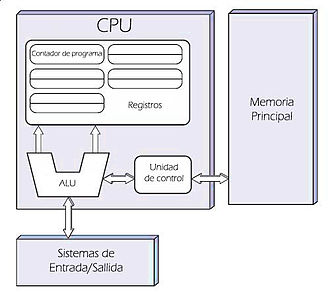
\includegraphics[scale=0.7]{Arquitecturaneumann}
  \caption{Arqutectura Neuman}
  \label{fig:arquitectura}
\end{figure}

Los ordenadores debe permitir recibir los datos a través de los dispositivos de entrada, y luego almacenarlos en la memoria principla para desde aqui comenzar un proceso de trasnformación utilizano en CPU; el CPU a la vez esta compuesto por la Unidad de control, la Unidad aritmática lógica y los registros que se encargar de realizar las operaciones ariméticas y lógicas, para brindar los resultados que vuelven a ser almanados en la memoria principal de donde son eviados a los dispisitivos de salida segun la necesidad.\\

Todos los elmentos de la arquitectura son utilizados en el proceso de ejecución de un programa es por eso que es encesario que el programador los tenga presenta:

\begin{itemize}
\item Dispositivos e entrada.
\item Memoria principal.
\item CPU.
  \begin{itemize}
  \item Unidad de control.
  \item Unidad lógica aritmética.
  \item Registros.
  \end{itemize}
\item Dispositivo de salida.
\end{itemize}



\subsubsection{Sistema de numeración}
\label{sec:sisnum}

Todos los ordenadores intenamento manejan la información en un formato binario, es así que la información analógica, ya sea esta en forma de texto, imagen, sonido, debe ser trasformado por el dispositivo de entrada en su representación binaria para ser posteriormente almacenado en la memoria \cite{Francis2020}.

La memoria es una estructura que contiene datos en forma de direcciónes y valores:

\begin{figure}[H]
  \centering
  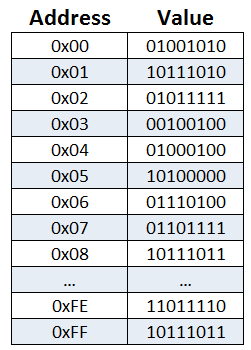
\includegraphics[scale=0.7]{memoria}
  \caption{Representación de la memoria}
  \label{fig:memoria}
\end{figure}



\subsubsection{Los lenguaje de programación}
\label{sec:lenguajes}
Cuando ya hablamos del contenido de la memoria, estamos hablando del software; el software que trabajo junto con el hardware de un computadora se lo clasifica en Sistema Operativo y Aplicativo; los dos se diferecia por el tipo de función que realiza.\\

El Sistema Operativo, tiene como función el control del hardware, para el diseño de esta software lo que interesas es lo que hace y como lo hace por que no estan orientado al usuario, pero por el contrario el software aplicativo a mas de su funcionalidad es necesario su apariencia. 

\begin{figure}[H]
  \centering
  
\includegraphics[scale=0.5]{lenguaje}
  \caption{Representación de la memoria}
  \label{fig:memoria}
\end{figure}



\newpage
\subsubsection{Preguntas de autocontrol}
\label{sec:preg-de-autoc-1}


\begin{itemize}
\item \textbf{Pregunta \# 1:} ¿Porqué C++ se utiliza para dar los fundamentos de la progración.
  \begin{itemize}
  \item  Es la base de todos los lenguajes. 
  \item Todo se puede hacer con c++.
  \item Tiene un curva de aprendizaje menos pronunciada.
  \end{itemize}

\item \textbf{Pregunta \# 2:} ¿Por qué el ordenador intenamente sulo puede manejar números binarios?.
  \begin{itemize}
  \item Es más facil de entender.
  \item El hardware solo maneja niveles de voltajes.
  \item Los calculos son más rapidos con números binarios.
  \item Ninguna de las anteriores.
  \end{itemize}
\item \textbf{Pregunta \# 3:} ¿Por qué la memoria principal no puede sustituir al registro
  \begin{itemize}
  \item Es muy grande.
  \item Es muy lenta.
  \item Es volatil. 
  \end{itemize}
\item \textbf{Pregunta \# 4:} ¿A que número decimal equivale el siguiente numero binario 10100101?.
  \begin{itemize}
  \item 200
  \item 250.
  \item $165_{10}$.
  \end{itemize}
\end{itemize}



\newgeometry{hmargin=2cm,vmargin=2cm,landscape}
\pdfpagewidth=297mm   %25in
\pdfpageheight=210mm %%16in
\textwidth=250mm
\textheight=190mm
\headwidth=\textwidth
\linewidth= 240mm




\begin{longtable}[H]{|b{0.5cm}|b{0.5cm}|b{0.5cm}|b{0.5cm}|b{0.5cm}|b{0.5cm}|b{10cm}|b{10cm}|}

\cabecera
  \multirow{3}{*}[-10ex]{\rotatebox{90}{TERCERA SEMANA}}  &  \multirow{3}{*}[-10ex]{\rotatebox[origin=c]{90}{13-septiembre-2021}}& \multirow{3}{*}[-10ex]{\rotatebox{90}{17-septiembre-2021}} & 2& & C& \multicolumn{2}{c|}{\semanaCA} \\ \cline{4-8}  
  &  &   & 2 & &C& \multicolumn{2}{c|}{\semanaCB} \\ \cline{4-8}
  &  &   & 2 & &C& \multicolumn{2}{c|}{\semanaCC} \\ \hline

\end{longtable}

\newpage
\restoregeometry

\subsubsection{Introducción a Linux y termux}
\label{sec:introduccion-linux-y}

Linux es un sofware que se distribuye libremente cuyo código es abierto, gracias a esta caracteristicas de distribución se han creados muchas versiones del Sistema Operativo entre la que tenemos Ubuntu, Fedliza Suselinux, etc.\\ 

\begin{tabular}[H]{|l|lm{8cm}|}
  \hline
  Año & Personaje & Contribución \\ \hline \hline
                    
  1983 & Richard Stallman & Crea el proyecto de GNU para crear un sistema operativo libre \\
  1989 & Richard Stallmen & Escribe la primera versión de la licencia GNU GPL \\
  1991 & Linux Torvalds &  La primera versión pública del núcleo de linux en un servidor ftp \\
  1992 & Linux Torvalds & Licencia el núcleo de Linux bajo GNU GPL \\
  1993 &  Más de 100 desarrolladores & Trabajan el núcleo Linux, y se crea un gran spectro, tambien se inicia a desarrollar wine \\
  1994 & Linux Torvalds & Presenta la version 1.1 de Linux. Red Hat y SUSE tamien presenta su version 1.1 \\
  1995 & DEC y SUN SPARC &Linux funciona en DEC y SUN SPARC \\ \hline
  2000 & StarOffice &La suite StarOffice es ofrecida segun los terminos de GNU GPL.\\
  2002 & OpenOffice.org &La comunidad OpenOffice.org libera la version 1,0; tambien el navegador web libre Mozilla. \\ \hline
\end{tabular}
\vfill

\subsubsection{Comando/Paquetes de linux: Instalación, configuración y prácticas de uso}
\label{sec:paquetes-de-linux}

El sistema operativo linux tiene la ventana de comando al cual se le da comandos, que actuan como ordenes que ejecuta el nucleo del sistema, algunos progras son llamandos por su nombre, es decir que al colocar su nombre en la linea de comando esta actua como un comando que llama al programa.\\

\begin{tabular}[H]{|l|m{11cm}|}
  \hline
  Comando/paquete & Descripción  \\ \hline \hline
  pwd & Comando para ver en que directorio se encuentra \\ \hdashline
  ls & Comando para listar directorio y archivos \\ \hdashline
  cd & Comando para ingresar a salir de directorio \\ \hdashline
  mkdir & Comando para crear un directorio nuevo   \\ \hdashline
  mv & Comando para mover un archivo o directorio a otra ubicación, también sirve para cambiar el nombre de archivos o directorios. \\ \hline \hline
  tree & \makecell[l]{Paquete y comando para ver el contenido en forma de arbol \\ debe instalarse con \textbf{pkg install tree}} \\ \hdashline
  vim & \makecell[l]{Paquete y comando para crear y editar archivos \\ debe instalarse con \textbf{pkg install vim}} \\ \hdashline
  clang & Compilador de c++\\   \hline
\end{tabular}

\newpage
.
\vspace{1cm}\\
\begin{tcolorbox}[skin=widget,
boxrule=1mm,
coltitle=black,
colframe=blue!45!white,
colback=blue!15!white,
width=(1\linewidth),before=\hfill,after=\hfill,
adjusted title={{\Large Actividad C1-1}:\textbf{Taller sobre el uso de termux}}]
Tiempo estimado para realizar esta actividad: 5 horas
\tcblower
Grabar un video tutorial sobre el  \textbf{Taller sobre termux}, en el cual se explique los pasos que están detallados en esta guía.\\ 

El entregable es un video subido al canal de youtube y luego compartido en la plataforma ClassRoom \\

Para ser evaluada esta actividad se utilizara la rubrica del anexo \#1.


\end{tcolorbox}



\subsubsection{Taller: Utilización de termux en la programación}
\label{sec:tall-util-de}


\paragraph{Objetivo:}
Utilizar con agilidad los comandos mkdir, rm, mv, cd;  para crear, borrar, mover y movilizarse entre los directorio.


\begin{enumerate}
  \item Verificar en que directorio se encuentra usted ubicado.
  \begin{tcolorbox}[colback=gray!5]
   \$ pwd
  \end{tcolorbox}
  \item Asegurarse que esté en el directorio de trabajo del  usuario  {\Large $\sim$} 
  \begin{tcolorbox}[colback=gray!5]
   \$ cd $\sim$
 \end{tcolorbox}
 %---------------------------------------------------------------
 \begin{shadedbox}
   \textcolor{white}{{\large \textsw{Creando directorios}}}
   \end{shadedbox}

 

 %---------------------------------------------------------------

  \item Crear un nuevo directorio con el nombre \textbf{Mis\_musicas}
  \begin{tcolorbox}[colback=red!5!white,colframe=red!75!black,fonttitle=\bfseries]
    \$ mkdir Mis\_musicas
  \end{tcolorbox}
  \item Crear un nuevo directorio con el nombre \textbf{Mis\_peliculas}
  \item Crear un nuevo directorio con el nombre \textbf{Mis\_fotos}
  \item Crear un nuevo directorio con el nombre \textbf{Mis\_tareas}
  \item Crear un nuevo directorio con el nombre \textbf{Mis\_documentos}
  \item Crear un nuevo directorio con el nombre \textbf{Otra\_informacion}
  
  \item Listar los directorios creados en una vista simple.
  \begin{tcolorbox}[colback=red!5!white,colframe=red!75!black,fonttitle=\bfseries]

    \$ \textbf{ls}
  \end{tcolorbox}
  \item Listar los directorios creados para ver la fecha de creación.
  \begin{tcolorbox}[colback=red!5!white,colframe=red!75!black,fonttitle=\bfseries]
    \$ \textbf{ls -l}
  \end{tcolorbox}
 %---------------------------------------------------------------
 \fbox{{\Large Creando subdirectorios:}} \rule{4cm}{0.4pt}
 %---------------------------------------------------------------
 \item ingresar al directorio \textbf{Mis\_musicas}
  \begin{tcolorbox}[colback=red!5!white,colframe=red!75!black,fonttitle=\bfseries]
    \$ cd Mis\_musicas
  \end{tcolorbox}
 
  \item Verificar que estamos dentro del directorios
 \begin{tcolorbox}[colback=red!5!white,colframe=red!75!black,fonttitle=\bfseries]
    \$ pwd
  \end{tcolorbox}
  
\item Crear un nuevo directorio con el nombre \textbf{Salsa}
  \begin{tcolorbox}[colback=red!5!white,colframe=red!75!black,fonttitle=\bfseries]
    \$ mkdir Salsa
  \end{tcolorbox}
  \item Crear un nuevo directorio con el nombre \textbf{Romantica}
  \item Crear un nuevo directorio con el nombre \textbf{Clasica}
  \item Crear un nuevo directorio con el nombre \textbf{Vallenato}
  \item Listar los directorios creados en una vista simple para
  verificar que los directorios han sido creados.
  \begin{tcolorbox}[colback=red!5!white,colframe=red!75!black,fonttitle=\bfseries]
    \$ \textbf{ls}
  \end{tcolorbox}
  \item Retorne al directorio de trabajo, puede utiliza cualquier de
  los dos comandos siguiente. \\
  
  \begin{minipage}[H]{0.5\linewidth}
  \begin{tcolorbox}[colback=red!5!white,colframe=red!75!black,fonttitle=\bfseries]
    \$ \textbf{cd ..}
  \end{tcolorbox}
  \end{minipage}
  \begin{minipage}[H]{0.5\linewidth}
  \begin{tcolorbox}[colback=red!5!white,colframe=red!75!black,fonttitle=\bfseries]
    \$ \textbf{cd} $\sim$
  \end{tcolorbox}
  \end{minipage}

  \item Utilizar el comando \textbf{tree} para ver todos los
  directorios y subdirectorio al mismo tiempo.
 \begin{tcolorbox}[colback=gray!5]
    \$ tree
   \end{tcolorbox}

   
   \item De la misma manera ingrese a los demás directorios y cree
   como mínimo dos subdirectorio con el nombre que usted crea
   conveniente.\\

 %---------------------------------------------------------------

 \begin{shadedbox}
   \textcolor{white}{{\large \textsw{Mover directorio dentro de otros directorio}}}
   \end{shadedbox}

 

 %---------------------------------------------------------------
  \item Asegurarse que esté en el directorio de trabajo del  usuario  {\Large $\sim$} 
  \begin{tcolorbox}[colback=gray!5]
   \$ cd $\sim$
 \end{tcolorbox}

  \item Haciendo el analisis de los contenido de los directorio
  creados, se llega a la conclusión que el directorio  \textbf{Mis\_tareas} debe esta dentro de directorio
  \textbf{Mis\_documentos}; mueva el directorio con el comando.
  
  \begin{tcolorbox}[colback=gray!5]
    \$ mv  Mis\_tareas  Mis\_documentos/
  \end{tcolorbox}


   \item Verifique la acción realizada con  el comando \textbf{tree} para ver todos los directorios.
 \begin{tcolorbox}[colback=gray!5]
    \$ tree
   \end{tcolorbox}
   \item Se ha llegado a la conclusión que el  directorio llamado
   \textbf{Otra\_informacion}. no va a ser utilizado por eso hay que eliminarlo.
 \begin{tcolorbox}[colback=gray!5]
    \$ rm -r Otra\_informacion
   \end{tcolorbox}

   si revias con {\it ls} el directorio ya no existe.
    %---------------------------------------------------------------

   
   \begin{shadedbox}
   \textcolor{white}{{\large \textsw{Cambiar los nombres de directorios:}}}
   \end{shadedbox}
 %---------------------------------------------------------------
  \item Asegurarse que esté en el directorio de trabajo del  usuario  {\Large $\sim$} 
  \begin{tcolorbox}[colback=gray!5]
   \$ cd $\sim$
 \end{tcolorbox}

\item Se decide cambiar el nombre de los directorio creados a nombre mas simples\\
  Mis\_musicas  simplemente  Musicas\\
  \begin{tcolorbox}[colback=gray!5]
    \$ mv  Mis\_musicas  Musica
  \end{tcolorbox}

  Mis\_fotos  simplemente Fotos\\
  \begin{tcolorbox}[colback=gray!5]
    \$ mv  Mis\_fotos  Fotos
  \end{tcolorbox}
  Mis\_tareas simplemente Tareas\\
  \begin{tcolorbox}[colback=gray!5]
    \$ mv  Mis\_tares  Tareas
  \end{tcolorbox}
  Mis\_documentos simplemente Documentos\\
  \begin{tcolorbox}[colback=gray!5]
    \$ mv  Mis\_documentos  Documentos
  \end{tcolorbox}
  

  
  



    
 \end{enumerate}



\newpage
\subsubsection{Preguntas de autocontrol}
\label{sec:preg-de-autoc-2}



\begin{itemize}
\item \textbf{Pregunta \# 1:} ¿Porqué C++ se utiliza para dar los fundamentos de la progración.
  \begin{itemize}
  \item  Es la base de todos los lenguajes. 
  \item Todo se puede hacer con c++.
  \item Tiene un curva de aprendizaje menos pronunciada.
  \end{itemize}
\item \textbf{fase \# 2:} El comando mv permite.
  \begin{itemize}
  \item Mover un directorio a otrade ubicación.
  \item Manejar toda la información que genera el proceso académico (silabos, módulos, tareas, etc.)
  \item Control de cumplimiento de actividades de acuerdo a un cronograma.
  \item Ingreso y difusión de calificaciones.
  \end{itemize}
\item \textbf{fase \# 3:} El comando mkdir permite.
  \begin{itemize}
  \item Cambiar el nombre de un directorio. 
  \item Crear un directorio nuevo.
  \item Eliminar un directorio.
  \item Ninguna de las anteriores.
  \end{itemize}
\item \textbf{fase \# 4:} Indique cuan de las siguinte sentencias es correcta para el comando cd ~.
  \begin{itemize}
  \item  Este comando es un ataja para ir directamente a la raiz del sistemas de archivo.
  \item  Este comando permite crear un directorio con nombre  ~.
  \item  Este comando es un atajo para ir directamente a directorio home.
  \item Ninguna de las anteriores es correcta.
  \end{itemize}
\end{itemize}



\newgeometry{hmargin=2cm,vmargin=2cm,landscape}
\pdfpagewidth=297mm   %25in
\pdfpageheight=210mm %%16in
\textwidth=250mm
\textheight=190mm
\headwidth=\textwidth
\linewidth= 240mm

\newpage
\begin{longtable}[H]{|b{0.5cm}|b{0.5cm}|b{0.5cm}|b{0.5cm}|b{0.5cm}|b{0.5cm}|b{10cm}|b{10cm}|}
\cabecera
\multirow{3}{*}[-10ex]{\rotatebox{90}{CUARTA SEMANA}}  & \multirow{3}{*}[-10ex]{\rotatebox[origin=c]{90}{20-septiembre-2021}}& \multirow{3}{*}[-10ex]{\rotatebox{90}{24-septiembre-2021}} & 2& &C&  \multicolumn{2}{c|}{\semanaDA} \\ \cline{4-8} 
  &  &   &2& &C&   \multicolumn{2}{c|}{\semanaDB} \\ \cline{4-8}
  &  &   &2& &C&  \multicolumn{2}{c|}{\semanaDC} \\ \hline

  \end{longtable}

\newpage
\restoregeometry

\subsubsection{Introducción a Vim y sus comandos}
\label{sec:introduccion-vim-y}

Seleccionar un entono de desarrollo que se adecue a las condiciones y
preferencias del programador es una de las primeras cosas que debe
haberse realizado para empezar la emocionante tarea de la programación.\\

Este capítulo describe las funciones más importantes de uno de los
primeros editores de texto creado para funcionar con el Sistemas
Operativo linux, el cual se ha mantenido y evolucionado para competir
con editores de texto que trabajan en entorno gráfico. \textbf{VI} era
el nombre como inicialmente se
lo conoció, pero que actualmente ha sido renombrado com  \textbf{VIM} para
indicar que es una versión modificada, que aunque sigue siento para
trabajar en modo texto también funciona para interfaces gráfica y
tanto en la de texto como en la gráfica su principal potencial es
cuando se lo utiliza únicamente con el manejo del teclado.\\

VIM fue un editor de texto, creado al inicio para ser el editor
predeterminado de la ventana de comando de UNIX, inicialmente sirvió para
poder crear y visualizar archivos de texto plano y muy cortos, pero
posteriormente su uso se fue expandiendo hasta convertirse en un
editor de texto avanzado utilizado como entorno de desarrollo para
crear código en varios de los lenguajes de programación más
importantes.\\

Su ejecución es simple solo hay que llamar a la ventana de comandos y
escribir su nombre.
\begin{tcolorbox}[colback=red!5!white,colframe=red!75!black,fonttitle=\bfseries]
\$ vim
\end{tcolorbox}

La principal característica de vim es que utiliza combinaciones de
teclas y es un programa de tipo modal.

\begin{itemize}
  \item \textbf{Modo normal o de comando:} Se podría decir que el modo normal de Vim es el estado de reposo. Otros editores de texto pasan la mayor parte del tiempo en lo que a Vim equivale al modo insertar. Para alguien que acaba de llegar a este editor modal, puede parecer extraño que pasemos la mayor parte del tiempo en el modo normal.
  \item \textbf{Modo de inserción:} En modo inserción cuando se pulsan las teclas se edita el texto como en otros editores. Se puede cambiar del modo comandos al modo inserción pulsando la tecla i. Hay un gran abanico de comandos para pasar al modo inserción, que difieren sustancialmente, pues permiten por ejemplo editar al final de la línea, en un punto concreto del texto, editar borrando una palabra, entre muchas otras. Un usuario experto puede sacar un gran provecho de la existencia de esta variedad de órdenes.
  \item \textbf{Modo visual:}Este modo es una mejora respecto a vi. Mediante unas ciertas combinaciones de teclas en combinación con las teclas de movimiento del cursor, se puede marcar un área de texto, ya sea un grupo de líneas o un bloque. Una vez se tiene el texto marcado se pueden usar órdenes del modo comandos para manipularlo. Las operaciones que se pueden realizar en este modo son más simples que las del modo comandos.
  \item \textbf{Modo linea de ordenes:} A este modo se accede pulsando la tecla dos puntos :. Tras los dos puntos se pueden introducir órdenes complejas, como por ejemplo buscar y reemplazar con expresiones regulares. Pulsando la tecla Esc se puede volver al modo órdenes. Las búsquedas se pueden realizar con la orden / (hacia adelante) y ? (hacia atrás). También se pueden filtrar líneas mediante.
\end{itemize}


\begin{figure}[H]
  \centering
  
\includegraphics[scale=0.6]{vim}
  \caption{Vim un editor de texto y entorno de desarrollo muy potente }
  \label{fig:vim}
\end{figure}


\textbf{Ventajas}\\

Fondo de escritorio con el logotipo de Vim.
La mayoría de los usuarios que usan Vim aseguran que este editor incrementa su productividad comparándolo con editores más simples una vez se ha superado la curva de aprendizaje. Las combinaciones de teclas se pueden memorizar empleando métodos mnemotécnicos, pues guardan relación con palabras inglesas. La complejidad intrínseca de aprender las instrucciones se ve recompensada por la mejora en la eficiencia. Los usuarios expertos pueden, usando unas pocas combinaciones de teclas, copiar texto, formatearlo u ordenarlo de muchas formas diferentes, que sólo se pueden realizar en la mayoría de editores mediante operaciones considerablemente más complejas. Basta con un poco de experiencia para notar que las combinaciones de instrucciones que permiten ediciones de texto complejas se facilitan con Vim.

\section{Vim en modo normal}
\label{sec:vim-en-modo}

Usar Vim es una experiencia completamente distinta a usar cualquier
otro editor de código. Vamos a hacer una breve demostración. Se
utiliza una sintaxis de verbo-modificador-objeto.  Empezamos en el
modo normal, pulsaremos i ( entrar al modo insertar) para introducir
unos cuantos párrafos de texto, pulsamos \textbf{Esc} para volver al
modo normal y aquí empieza la magia. No os preocupis, iremos mirando
cada uno de ellos en detalle en los próximos post, pero podeis
echándole un vistazo.
Aprende algunos verbos: v(visual), c(change/cambiar),
d(delete/borrar), y(yank/copiar).\\

Aprende algunos modificadores: i(inside/dentro de), a
(around/alrededor), t (till/ hasta que encuentra el carácter). f (find
/hasta que encuentra el carácter incluyendolo), / (buscar).\\
Aprender algunos objetos: w (word/palabra), s (sentencia/frase), p
(paragraphs/párrafo), t (tag/ para html/xml). \\

Los principales comandos utilizados en modo de comando son:

\begin{table}[H]
  \centering
  \begin{tabular}[H]{rl}
    \hline
    Comando&Descripción \\ \hline
    ESC & Se asegura que VIM este en modo de comandos\\
    i  & cambia del modo de comando a modo de inserción \\
    a  & cambia del modo de comando a modo de inserción \\
    h & mover una fila hacia arriba \\
    l & mover una fila hacia abajo \\
    j & mover un espacio a la izquierda \\
    k & mover un espacio a la derecha \\
    dd &  Eliminar la linea actual de texto.\\
    yy &  copiar una linea \\
    p & pegar la linea copiada\\
         G& Mover el cursor al final del archivo. \\
    gg &  Mover el cursor al inicio del archivo \\
    G & Mover el cursos al final del archivo\\
    / & preparar a VIM para buscar una palabra\\
    :s/hola/cola/g &remplar la palabra hola conla palabra \\
    : & se prepara a VIM para recibir un comando\\
    :set number & mostrar la numeración de cada linea \\
    0 & mover el cursor al inicio de la linea \\
    \$ & Mover el cursor al final de la linea\\ \hline
    
  \end{tabular}
  \caption{Comandos frecuentemente utilizados en la edición con VIM}
  \label{tab:comandovim}
\end{table}

\paragraph{VIM en modo insertar
}


A este modo se puede ingresar presionando cualquiera de las siguientes
letras (i,I,o,O,c,C) estando en modo se puede insertar o modificar el
texto.






\newpage
\begin{tcolorbox}[skin=widget,
boxrule=1mm,
coltitle=black,
colframe=blue!45!white,
colback=blue!15!white,
width=(1\linewidth),before=\hfill,after=\hfill,
adjusted title={{\Large Actividad C1-2}:\textbf{Taller sobre el uso de vim}}]
Tiempo estimado para realizar esta actividad: 5 horas
\tcblower
Grabar un video tutorial sobre el  \textbf{Taller sobre vim}, en el cual se explique los pasos que están detallados en esta guía.\\ 

El entregable es un video subido al canal de youtube y luego compartido en la plataforma ClassRoom \\

Para ser evaluada esta actividad se utilizara la rubrica del anexo \#1.


\end{tcolorbox}



\subsubsection{Taller uso de vim: Creación y edición de archivos}
\label{sec:ejerc-pract-con}


\begin{enumerate}
  \item Ingrese al directorio \textbf{Tareas}, utilizando el siguiente comando.
    \begin{tcolorbox}[colback=gray!5]
    \$ cd \textbf{$\sim$/Tareas}
  \end{tcolorbox}

  \item  Cree un directorio llamado \textbf{Practica1}.
    \begin{tcolorbox}[colback=gray!5]
    \$ mkdir Practica1
  \end{tcolorbox}

  \item Ingrese al directorio \textbf{Practica1}.
    \begin{tcolorbox}[colback=gray!5]
    \$ cd Practica1
  \end{tcolorbox}

  \item Crear un nuevo archivo llamado \textbf{suma.cpp} con el editor \textbf{vim}, utilice  la siguiente qqinstrucción.
    \begin{tcolorbox}[colback=gray!5]
    \$ vim suma.cpp
  \end{tcolorbox}
  
  \item Pulsa la tecla \fbox{\Large i} (para entrar en el modo edición que permite  escribir)
  \item Escribir el siguiente texto sin dejar lineas en blanco:
\begin{verbatim}
#include<iostrema>
using namespace std;
int main()
{
 float A,B,C;
 cin>>A>>B;
 C=A+B;
cout<<C;
return 0;
}
\end{verbatim}

  \item Hemos acabado de escribir, salimos del modo edición presionando
  la tecla \fbox{\Large ESC}.
  \item Ingresamos al modo comando presionando la tecla que contiene los dos punto
  \fbox{\Large :}
\item Grabar escribiendo \fbox{\Large w} minúscula.

  
  \item Vuelve al modo comando con dos puntos \fbox{\Large :} y salga
  de vim escribiendo \fbox{\Large q} minúscula.
  \item Lista los archivos que hay en el directorio actual (use ls  -l), y veraz el archivo \textbf{suma.cpp}.

  \item Genere el archivo ejecutable con el siguiente comando.

  
    \begin{tcolorbox}[colback=gray!5]
    \$ g++   suma.cpp   -o   suma
  \end{tcolorbox}

  \item Si no le presento ninguna error; lista los archivos que hay en el directorio actual (use ls
    -l).

  \item Ejecute el programa de la siguinte manera.
    
    \begin{tcolorbox}[colback=gray!5]
    \$ ./suma
  \end{tcolorbox}

  
\item Abra otra vez el archivo creado con el editor vim.
  \item Modifique su contenido para que quede de la siguiente manera:

\begin{Verbatim}[commandchars=\\\{\}]
#include<iostrem>
using namespace std;
int main()
\{
float A,B,C;
\textcolor{red}{cout<<"Ingrese 2 numero A B :";}
cin>>A>>B;
C=A+B;
\textcolor{red}{cout<<"El resultado es :";}
cout<<C;
return 0;
\}
\end{Verbatim}


\item Para modificarlo siga las siguientes instrucciones.
\item Muestre el número de las lineas escribiendo el comando
    \begin{tcolorbox}[colback=gray!5]
    : set number
  \end{tcolorbox}
\item Asegure que esta al inicio del archivo con \fbox{\Large  ESC} y
luego escribe \fbox{\Large gg} en minúscula.
\item Valla a la novena línea escribiendo \fbox{\Large :}
\fbox{\Large 9}.
\item Cree una nueva linea en la parte superior con la tecla \fbox{\Large
  O} mayúscula.
\item Escriba la siguiente linea y vuelva al modo de comando con ESC.
\begin{Verbatim}[commandchars=\\\{\}]
\textcolor{red}{cout<<"El resultado es :";}
\end{Verbatim}
\item Asegurese de estar en el modo comando presionando la tecla \fbox{\Large  ESC}.
  
\item Valla a la quinta línea escribiendo \fbox{\Large :}
\fbox{\Large 5}.
\item Abra una nueva linea en la parte inferior con la tecla
\fbox{\textbf{o}} minúscula.
\item Escriba la siguiente linea y vuelva al modo de comando presionando 
\fbox{\Large ESC}.

\begin{Verbatim}[commandchars=\\\{\}]
\textcolor{red}{cout<<"Ingrese 2 numero separados de espacio A B :";}
\end{Verbatim}

\item Modifique la antepenultima linea.

\begin{Verbatim}[commandchars=\\\{\}]
cout<<C\textcolor{red}{<<endl;}
\end{Verbatim}


  

\item Ahora vamos a cambiar la letra  \textbf{A}  por \textbf{x} escribiendo el siguiente
comando.
    \begin{tcolorbox}[colback=gray!5]
   {\Large :1,\$s/A/x/g}
  \end{tcolorbox}

 
\item De la misma manera cambien la letra \textbf{B}  por la letra \textbf{y} escribiendo el siguiente comando.
  
\textbf{Masculino}.
    \begin{tcolorbox}[colback=gray!5]
   {\Large :1,\$s/B/y/g}
  \end{tcolorbox}


\item De la misma manera cambie la  letra \textsf{C} por la letra \textbf{z} con el siguiente comando.
\textbf{Masculino}.
    \begin{tcolorbox}[colback=gray!5]
   {\Large :1,\$s/C/z/g}
  \end{tcolorbox}

\item Finalmente obtenemos el siguiente contenido modificado.
  
\begin{Verbatim}[commandchars=\\\{\}]
#include<iostrem>
using namespace std;
int main()
\{
float x,y,z;
\textcolor{red}{cout<<"Ingrese 2 número separados de espacio x y :";}
cin>>x>>y;
z=x+y;
\textcolor{red}{cout<<"El resultado es :";}
cout<<z\textcolor{red}{<<endl;}
return 0;
\}
\end{Verbatim}
\item Asegurese de que esta en el modo de comando presionando la tecla \textbf{ESC}:
\item Entra en el modo comando apretando la tecla dos puntos:
\item Grabar \fbox{\Large w}.
\item Vuelve al modo comando y con \fbox{\Large :} \fbox{\Large q}.

  \item Lista los archivos que hay en el directorio actual (use ls
  -l).

  \item Genere el archivo ejecutable.

  
    \begin{tcolorbox}[colback=gray!5]
    \$ g++   suma.cpp   -o   suma
  \end{tcolorbox}

  \item Si no le presento ninguna erro lista los archivos que hay en el directorio actual (use ls
    -l).

  \item Ejecute el programa para ver como se ve con los cambios realizados.
    \begin{tcolorbox}[colback=gray!5]
    \$ ./suma
  \end{tcolorbox}

\end{enumerate}





\newpage
\subsubsection{Preguntas para el autocontrol}
\label{sec:preguntas-para-el}




\begin{itemize}
\item \textbf{Pregunta \# 1:} ¿Cúal es la modalidad que permite darle ordenes a vim?.
  \begin{itemize}
  \item  edición
  \item commado
  \item vista
  \end{itemize}
\item \textbf{fase \# 2:} ¿Cuales son las letras que me permite mover verticalmente?.
  \begin{itemize}
  \item a,b
  \item j,k
  \item h,l.
  \item Ninguna de las anteriores.
  \end{itemize}
\item \textbf{Pregunta \# 3:} ¿Cúal es la o las  letra que permite ir al inicio del archivo?.
  \begin{itemize}
  \item G
  \item gg.
  \item s. 
  \end{itemize}
\item \textbf{Pregunta \# 4:} ¿Cúal es la tecla que permite y al final de la linea?.
  \begin{itemize}
  \item 0.
  \item l.
  \item \$.
    \end{itemize}
\item \textbf{Pregunta \# 4:} ¿Cúal es la tecla que permite remplazar una letra?.
  \begin{itemize}
  \item 0.
  \item r.
  \item \$.

  \end{itemize}
\end{itemize}




\newgeometry{hmargin=2cm,vmargin=2cm,landscape}
\pdfpagewidth=297mm   %25in
\pdfpageheight=210mm %%16in
\textwidth=250mm
\textheight=190mm
\headwidth=\textwidth
\linewidth= 240mm

\begin{longtable}{|m{3cm}@{\hspace{0.4cm}}|m{2.3cm}|m{\linewidth-6cm}|}
 
  \hline
  \rowcolor{gray!20}
  Actividad                  & Criterio                      & Nivel 1          \\ \hline
 \hline 
\endfirsthead
  
  \multicolumn{3}{@{}l}{\ldots Continuación} \\ \hline \hline
  \rowcolor{gray!20}
  
  Actividad                  & Criterio                      & Nivel 1          \\ \hline

 \hline
 \endhead
\hline
  \multicolumn{3}{r@{}}{\ldots Continua  \ldots} \\ 
  \endfoot
  \hline
  \endlastfoot

\rowcolor{green!50}                                       
\multicolumn{2}{l|}{Nota máxima } & \makecell[r]{100} \\ \hline

\multirow{3}{*}{ \actividadCA }        &\criterioCAA  & \nivelCAA  \\  \cline{2-3}
                                        & \criterioCAB & \nivelCAB   \\ \cline{2-3}
                                        & \criterioCAC & \nivelCAC   \\ \hline   
\end{longtable}


\newpage
\begin{longtable}[H]{|b{0.5cm}|b{0.5cm}|b{0.5cm}|b{0.5cm}|b{0.5cm}|b{0.5cm}|b{10cm}|b{10cm}|}
\cabecera
\multirow{3}{*}[-10ex]{\rotatebox{90}{QUINTA SEMANA}} & \multirow{3}{*}[-10ex]{\rotatebox[origin=c]{90}{27-septiembre-2020}}& \multirow{3}{*}[-10ex]{\rotatebox{90}{01-octubre-2021}} & 2 & &C & \multicolumn{2}{c|}{\semanaEA} \\ \cline{4-8}                       &                                                               &                                                    &2  & &C  & \multicolumn{2}{c|}{\semanaEB} \\ \cline{4-8} 
                       &                                                              &                                                    &2 &  &C  & \multicolumn{2}{c|}{\semanaEC} \\ \hline

\end{longtable}

\newpage
\restoregeometry

\subsubsection{Introducción a la programación}
\label{sec:intr-la-progr}

\section{Ciclo de vida del Software}
\label{sec:ciclovida}

Es importante enterder que el desarrollo de un software nunca termina pues siempre habran oportunidades de mejoras, es por eso que el proceso se convierte en un ciclo.

\begin{figure}[H]
  \centering
  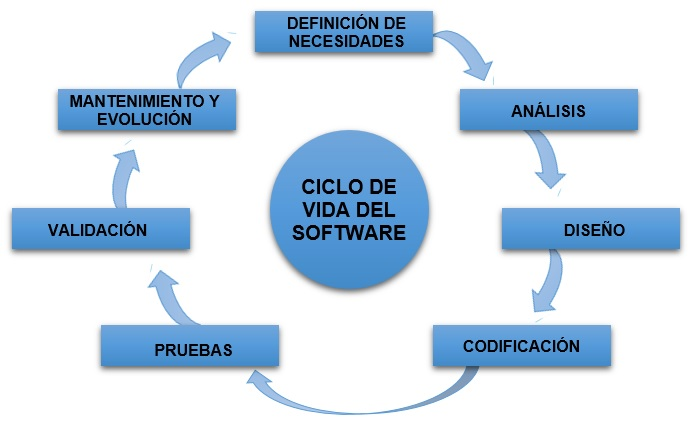
\includegraphics[scale=0.5]{ciclo}
  \caption{Ciclo de vida del Software}
  \label{fig:documentacion}
\end{figure}


\section{Creación del Software: Principios básicos.}
\label{sec:creac-del-softw}

La creación de software es un proceso interactivo que se realiza en
varias etapas.\\

\begin{minipage}[H]{0.45\linewidth}
  \begin{enumerate}
    \item Análisis del problema.
    \item Diseño del Algoritmo.
    \item Codificación.
    \item Compilación y ejecución.
  \end{enumerate}
  
\end{minipage}
\begin{minipage}[H]{0.45\linewidth}
  \begin{enumerate}
    \setcounter{enumi}{4}
    \item Verificación.
    \item Depuración.
    \item Mantenimiento.
    \item Documentación.
  \end{enumerate}
  
\end{minipage}


\subsection{El análisis y diseñó}
\label{sec:el-analisis-y}

El análisis del problema por lo general se lo realiza a la par que el
Diseño del Algoritmo, este se puede dar gracias a que los problemas
pequeños como los que se resuelven en este libro por lo general ya han
sido analizados por los estudiantes durante los procesos de estudios
que les precedió a este nivel académico (colegiatura), es por eso que
directamente se puede pasar al diseño de algoritmo utilizando
herramientas de diagrama de flujo para generar la secuencia de
instrucciones que servirán para llevarlas a un 
archivo  de texto con una sintaxis definida por un lenguaje de
programación en una siguiente etapa que se llama codificación.
\begin{figure}[H]
  \centering
  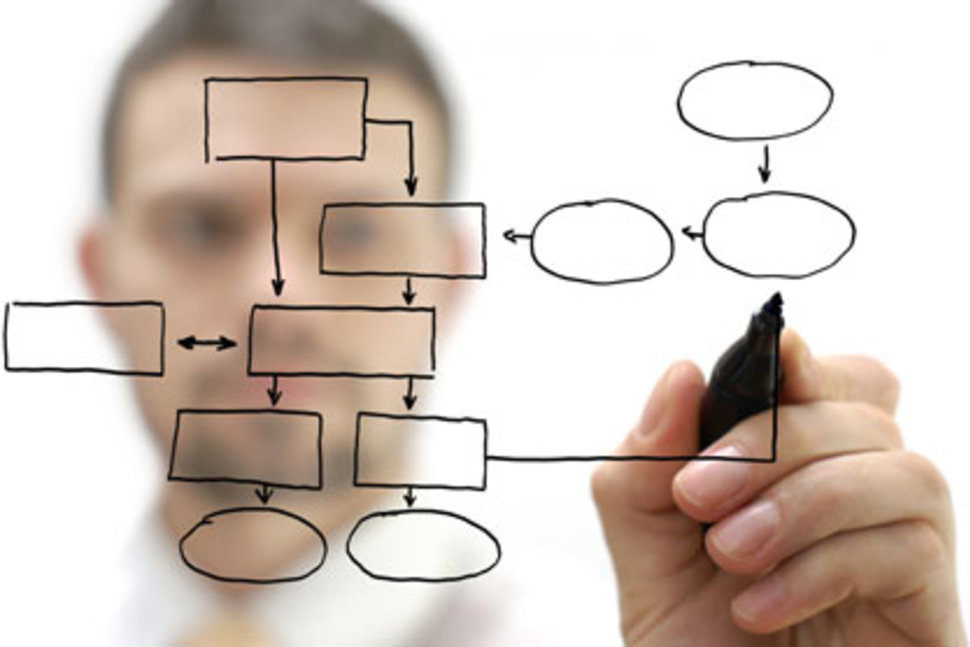
\includegraphics[scale=0.1]{analisis}
  \caption{Análisis y diseño}
  \label{fig:analisis}
\end{figure}


\subsection{La etapa de la codificación}
\label{sec:la-etapa-de}

En esta etapa, es donde el profesional informático o programador debe
hacer gala de su habilidad para escribir el conjunto de instrucciones
utilizando un conjunto de palabras reservadas aprendidas y memorizadas
en su proceso de capacitación, el lenguaje de programación como se
llama a este conjunto de palabras reservadas sera escogido en función
del tipo de problema a resolver, en este libro se escogió el C++ para
resolver problemas matemáticos; la codificación involucra crear un
archivo entendible en primera instancia por el programador.

\begin{figure}[H]
  \centering
  
\includegraphics[scale=0.2]{programador}
  \caption{Fase de codificación}
  \label{fig:codificacion}
\end{figure}

\subsection{La etapa de compilación y ejecución}
\label{sec:la-etapa-de-1}

Es necesario que el computador interprete cada linea de código que se
encuentra en el archivo creado en la etapa de codificación; después de
contar con el archivo, se recurre a un programa del sistema operativo
llamado compilador el cual en entorno linux es g++ este comando
convierte el archivo fuente de C++ en un archivo que contiene un
lenguaje entendible por la máquina, el cual posteriormente puede ser
ejecutado.

\begin{figure}[H]
  \centering
  
\includegraphics[scale=0.2]{running}
  \caption{Fase de compilación y ejecución}
  \label{fig:documentacion}
\end{figure}



\subsection{La etapa de verificación y depuración}
\label{sec:la-etapa-de-2}

Es muy difícil que un programa en su primera ejecución brinde los
resultados deseados por el usuario o programador más aun si se trata
de la resolución de un problema  antes no resuelto, es por eso que
después de una primera ejecución es necesario verificar que los
resultados sean los correctos. y si no es así comenzar la etapa de
DEPURACIón, la cual tiene como objetivo asegurar que el programa
obtenga la salida deseada.
\begin{figure}[H]
  \centering
  
\includegraphics[scale=0.2]{debugging}
  \caption{Fase de verificación y depuración}
  \label{fig:documentacion}
\end{figure}


\subsection{La etapa de mantenimiento}
\label{sec:la-etapa-de-3}

El software nunca termina de elaborarse  y es que por lo general el
programa a pesar de obtener las salidas deseadas, necesita
actualización en función de adaptarse a los cambios que se dan en su
entorno.
\begin{figure}[H]
  \centering
  
\includegraphics[scale=0.3]{MantenimientoSoftware}
  \caption{Fase de mantenimiento}
  \label{fig:documentacion}
\end{figure}

\subsection{Documentación}
\label{sec:la-etapa-de-4}
Aunque un programa elegantemente codificado utilizando las normas de
programación recomendadas en los standares, no necesita de mucha
documentación, si es verdad que la etapa de documentación es necesaria
para la evolución y transportabilidad de un programa.

\begin{figure}[H]
  \centering
  
\includegraphics[scale=0.3]{documentacion}
  \caption{Fase de documentación del Software}
  \label{fig:documentacion}
\end{figure}




\subsubsection{Taller de programación básica 1}
\label{sec:tall-de-progr}

\vfill

\subsubsection{Taller de programación 2: Elaboración de informe}
\label{sec:tall-de-progr-1}

\vfill

\begin{tcolorbox}[skin=widget,
boxrule=1mm,
coltitle=black,
colframe=blue!45!white,colback=blue!15!white,width=(1\linewidth),before=\hfill,after=\hfill,adjusted title={\textbf{Preguntas para el autocontrol}}]
Estan agrupadas por fases.  
\tcblower

\begin{itemize}
\item \textbf{Pregunta \# 1:} A quien se le atribuje la arquitectura del computador.
  \begin{itemize}
  \item  char babage.
  \item Jhon Vom Neumann.
  \item Rober Noise.
  \end{itemize}
\item \textbf{fase \# 2:} Dar seguimiento al proceso académico de las asignaturas.
  \begin{itemize}
  \item Llevar el control de asistencia tanto de maestrantes como de docentes.
  \item Manejar toda la información que genera el proceso académico (silabos, módulos, tareas, etc.)
  \item Control de cumplimiento de actividades de acuerdo a un cronograma.
  \item Ingreso y difusión de calificaciones.
  \end{itemize}
\item \textbf{fase \# 3:} Gestionar la información académica.
  \begin{itemize}
  \item Repositorio digital.
  \item Control de carga y descarga de información al Repositorio.
  \item Busqueda de información. 
  \end{itemize}
\item \textbf{fase \# 4:} Manejar la relación con los maestrantes y docente.
  \begin{itemize}
  \item Integración con Microsoft Team y Google ClassRoom.
  \item Integración con Microsoft Team y Google ClassRoom.
  \item Integración con Microsoft Team y Google ClassRoom.
  \end{itemize}
\end{itemize}

\end{tcolorbox}




\newgeometry{hmargin=2cm,vmargin=2cm,landscape}
\pdfpagewidth=297mm   %25in
\pdfpageheight=210mm %%16in
\textwidth=250mm
\textheight=190mm
\headwidth=\textwidth
\linewidth= 240mm

\begin{longtable}{|m{3cm}@{\hspace{0.4cm}}|m{2.3cm}|m{\linewidth-6cm}|}
 
  \hline
  \rowcolor{gray!20}
  Actividad                  & Criterio                      & Nivel 1          \\ \hline
 \hline 
\endfirsthead
  
  \multicolumn{3}{@{}l}{\ldots Continuación} \\ \hline \hline
  \rowcolor{gray!20}
  
  Actividad                  & Criterio                      & Nivel 1          \\ \hline

 \hline
 \endhead
\hline
  \multicolumn{3}{r@{}}{\ldots Continua  \ldots} \\ 
  \endfoot
  \hline
  \endlastfoot

\rowcolor{green!50}                                       
\multicolumn{2}{l|}{Nota máxima } & \makecell[r]{100} \\ \hline
  \multirow{3}{*}{ \actividadAA }        &\criterioAAA  & \nivelAAA  \\  \cline{2-3}
                                        & \criterioAAB & \nivelAAB   \\ \cline{2-3}
                                        & \criterioAAC & \nivelAAC   \\ \hline   
\end{longtable}

\newpage
\begin{longtable}[H]{|b{0.5cm}|b{0.5cm}|b{0.5cm}|b{0.5cm}|b{0.5cm}|b{0.5cm}|b{10cm}|b{10cm}|}
\cabecera
\multirow{3}{*}{\rotatebox{90}{SEXTA SEMANA}}   & \multirow{3}{*}{\rotatebox[origin=c]{90}{04-octubre-2021}}& \multirow{3}{*}{\rotatebox{90}{08-octubre-2021}} &2&2&C& \multicolumn{2}{c|}{\semanaFA} \\ \cline{4-8}  
  &  &   & 2& &C & \multicolumn{2}{c|}{\semanaFB} \\ \cline{4-8} 
  &  &   & 2& &C & \multicolumn{2}{c|}{\semanaFC} \\ \hline

  \end{longtable}

\newpage
\restoregeometry

\subsubsection{Figuras para el diagrama de flujo}
\label{sec:ciclo-de-vida}




% Define block styles
\tikzstyle{decision} = [diamond, draw, fill=blue!20, 
    text width=3.5em, text badly centered, node distance=1.5cm, inner sep=0pt]
\tikzstyle{block} = [rectangle, draw, fill=blue!20, text centered, rounded corners, minimum
    height=1em, minimum width=0.5cm]
\tikzstyle{line} = [draw, -latex']
\tikzstyle{cloud} = [draw, ellipse,fill=red!10, node distance=2cm,
minimum height=2em]
\tikzstyle{conector}=[circle, scale=0.75, color=white, fill=blue!10]


    \tikzstyle{output1} = [signal, signal from=nowhere, signal to=east, minimum width=2cm, minimum height=0.5cm, text centered, draw=black, fill=blue!10]

    \tikzstyle{input1} = [signal, signal from=east, signal to=nowhere, minimum width=2cm, minimum height=0.5cm, text centered, draw=black, fill=red!30]
    


\begin{table}[H]
  \centering
  \begin{tabular}[H]{|p{4cm}|l|p{5cm}|}
    \hline
    Símbolo & Propósito & Descripción \\ \hline
    \begin{minipage}[H]{1.0\linewidth}

      \begin{center}
        \begin{tikzpicture}
          \node [cloud,yshift=1cm] (inicio){inio};
          \node [conector,below of=inicio,yshift=-0.5cm] (fin){x};
          \path [line] (inicio) -- (fin);
          
        \end{tikzpicture}
      \end{center}
    \end{minipage}
            &inicio & Indica el inicio de un programa. \\ \hline

 \begin{minipage}[H]{1.0\linewidth}

      \begin{center}
        \begin{tikzpicture}[node distance=1cm,auto]
          \node [conector] (ini){x};
          \node [input1,below of=ini] (inicio){Entrada};
          \node [conector,below of=inicio] (fin){x};
          \path [line] (ini) -- (inicio);
          \path [line]
          (inicio) -- (fin);
        \end{tikzpicture}
      \end{center}
    \end{minipage}
            &Entrada & Habilita el teclado(o dispositivo de entrada)
                       para ingresar datos \\ \hline
   
 \begin{minipage}[H]{1.0\linewidth}

      \begin{center}
        \begin{tikzpicture}[node distance=1cm,auto]
          \node [conector] (ini){x};
          \node [output1,below of=ini] (inicio){Salida};
          \node [conector,below of=inicio, yshift=-0.5cm] (fin){x};
          \path [line] (ini) -- (inicio); \path [line]
          (inicio) -- (fin);
        \end{tikzpicture}
      \end{center}
    \end{minipage}
            &Salida & Habilita la pantalla(o dispositivo de salida)
                      para presentar información al usuario) \\ \hline

    \begin{minipage}[H]{1.0\linewidth}

      \begin{center}
        \begin{tikzpicture}
          \node [conector] (ini){x};
          \node [decision,yshift=-0.2cm,below of=ini] (inicio){Decisión};
          \node [block,dashed,below of=inicio,yshift=-0.5cm] (fin){Proceso1};
          \node [block,dashed,below of=inicio,yshift=-0.5cm,xshift=2cm]
          (fin2){Proceso2};
          \node [conector, below of=fin] (inif){x};
         
          \path [line] (ini) -- (inicio);
          \path [line] (inicio) -| node[anchor=south] {yes} (fin2);
          \path [line] (inicio) -- node[anchor=east] {no} (fin);
          \path [line] (fin2) |- (inif);
          \path [line] (fin) -- (inif);
        \end{tikzpicture}
      \end{center}
      
    \end{minipage}
            &Decisión & Permite ejecutar de forma alternativa dos
                        procesos distintos. \\ \hline
    \begin{minipage}[H]{1.0\linewidth}

      \begin{center}
        \begin{tikzpicture}[node distance=1cm,auto]
          \node [conector] (ini){x};
          \node [block,below of=ini] (inicio){Proceso};
          \node [conector,below of=inicio] (fin){x};
          \path [line] (ini) -- (inicio);
          \path [line] (inicio) -- (fin);
        \end{tikzpicture}
      \end{center}
    \end{minipage}
            &Proceso & Indica especificamente una tarea que realiza el
                       CPU ya sea para realizar una operación
                       matemática, lógica de asignatura u otra \\ \hline
    \begin{minipage}[H]{1.0\linewidth}

      \begin{center}
        \begin{tikzpicture}[node distance=0.5cm,auto]
          \node [conector] (ini){x};
          \node [cloud,below of=ini,yshift=0.5cm] (inicio){fin};
          \path [line] (ini) --(inicio);
        \end{tikzpicture}
      \end{center}
    \end{minipage}
            &fin & Indica la finalización del programa \\ \hline

    
  \end{tabular}
  \caption{Simboles básicos utilizados para la creación de los diagrama de flujo}
  \label{tab:simbolos}
\end{table}





\subsection{Inicio/fin}
\label{sec:iniciofin}

Este símbolo indica el proceso que se realiza antes de empezar a
resolver el problema, el computador debe prepararse para la
utilización de dispositivos de entrada y salida, y es en esta etapa
donde se verifica que existen estos dispositivos y además están
disponibles.
\begin{center}
  \begin{tikzpicture}[node distance=2cm, auto]
  
    \node [cloud] (inicio) {inicio};
    \node [conector, below of=inicio] (con) {x};

    \node [cloud, right of =con,xshift=1cm] (fin) {fin};
    \node [conector, right of=inicio, xshift=2cm] (con2) {x};
  
    \path [line] (inicio) -- (con);
    \path [line] (con2) -- (fin);


  
  \end{tikzpicture}
\end{center}



\subsection{Símbolo de Proceso}
\label{sec:simbolo-de-proceso}

Informa que el computador esta ocupado realizando algún proceso que
por lo generar tiene que ver con operaciones matemáticas.

\begin{minipage}[H]{0.45\linewidth}
  \begin{center}
    \begin{tikzpicture}[node distance=2cm,auto]
      \node [conector] (up){x}; \node [block, below of=up] (proceso)
      {proceso};

      \node [conector, below of=proceso] (down){x};

      \path [line] (up) -- (proceso); \path [line] (proceso) --
      (down);
    \end{tikzpicture}
  \end{center}
\end{minipage}
\begin{minipage}[H]{0.45\linewidth}
  \begin{center}
    \begin{tikzpicture}[node distance=2cm,auto]
      \node [conector] (up){x}; \node [block, below of=up] (proceso)
      {r=a+b};

      \node [conector, below of=proceso] (down){x};

      \path [line] (up) -- (proceso) ;
      \path [line] (proceso) --   (down);
    \end{tikzpicture}
  \end{center}
\end{minipage}

\subsection{Símbolo de decisión}
\label{sec:simbolo-de-decision}

Este símbolo es utilizado en un punto en la secuencia de instrucciones
donde se necesita mostrar más de una acción a seguir para llegar a la
solución.

\begin{center}
  \begin{tikzpicture}[node distance=2cm,auto]
    \node [conector] (up){x};
    \node [decision, below of=up] (decision)  {decision};
    \node [block,dashed, below of=decision,yshift=-0.5cm] (proceso1)  {proeso 1};
    \node [block,dashed, right of=proceso1,xshift=2cm] (proceso2)  {proeso 2};

    
    \node [conector, below of=proceso1] (down){x};

    \path [line] (up) -- (decision);
    \path [line,dashed] (decision) -- node {yes} (proceso1);
    \path [line,dashed] (decision) -| node {no} (proceso2);
    \path [line,dashed] (proceso1) -- (down);
    \path [line,dashed] (proceso2) |- (down);

  \end{tikzpicture}
\end{center}
Estructura de repetición utilizando el simbolo de decisión.

\begin{center}
  \begin{tikzpicture}[node distance=2cm,auto]
    \node [conector] (up){x};
    \node [conector,right of= up,xshift=2] (up2){x};
    \node [block,dashed, below of=up] (proceso2)  {proceso 2};
    \node [decision, below of=proceso2] (decision)  {decision};
    \node [block,dashed, below of=decision,yshift=-0.5cm] (proceso1)  {proeso 1};

    
    \node [conector, below of=proceso1] (down){x};

    \path [line] (up) -- (proceso2);
    \path [line] (proceso2) -- (decision);
    
    \path [line,dashed] (decision) -- node {yes} (proceso1);
    \path [line,dashed] (decision) -| node[anchor=south] {no} (up2);
    \path [line,dashed] (proceso1) -- (down);
    \path [line,dashed] (up2) -- (up);

  \end{tikzpicture}
\end{center}




\subsection{Símbolo de entrada y salida}
\label{sec:simbolo-de-entrada}

Estos dos símbolo son utilizados frecuentemente, tanto al inicio (entrada) como al
final (salida) de la secuencia de instrucciones para obtetener los datos a procesar y para presentar los resultados; por lo general los datos de entrada son provistos por una fuente externa a la computadora (como es el teclado) y los resultados se los muestra también generalmente por el monitor o pantalla.

\begin{center}
  \begin{tikzpicture}[node distance=2cm, auto]

    
    \node [input1] (inicio) {Entrada}; \node [conector, below of=inicio]
    (con) {x};

    \node [output1, right of =con,xshift=2.5cm] (fin) {Salida}; \node [conector, right
    of=inicio, xshift=4cm] (con2) {x};
  
    \path [line] (inicio) -- (con); \path [line] (con2) -- (fin);


  
  \end{tikzpicture}
\end{center}




\subsubsection{Taller de Diagrama de flujo}
\label{sec:taller-de-diagrama}

\section{Resolviendo un problema muy simple}
\label{sec:resolv-un-probl}

Un problema muy simple que se presenta frecuentemente  en la vida de
las personas, es la resta o suma de dos número;  aunque restar o sumar dos
número (por ejemplo:  4--2=2) puede parecer un problema que no necesitaría la ayuda de un computador, cuando la resta o suma se realiza entre números que pasan de los dos dígitos (ejemplo: 994-930=64), al humano le toma un poco más de tiempo y trabajo hacerlo mentalmente, ya que el cerebro no ha sido diseñado para mantener en memoria la
información por mucho tiempo, y es ahí donde los computadores gracias
a la arquitectura de John Vonn Newman se vuelve en la mejor aliada.

\subsection{Análisis del problema}
\label{sec:analsis-del-problema}

En el momento que tus oídos escuchan un problema, tu mente de forma
automática va intentar encontrar la solución, comenzando a elaborar un
conjunto de instrucciones posibles para obtener esta solución; en el
problema planteado las siguientes son instrucciones que aunque de
forma no muy precisa  nos da una  solución  que podemos mejorar con el
conocimiento de las técnicas enseñadas en la asignatura de fundamentos
de programación.

  \begin{tcolorbox}[title=''Algoritmo para restar dos números'', colback=red!5!white,colframe=red!75!black,fonttitle=\bfseries]
    \begin{enumerate}
      \item Conseguir el primer número.
      \item Conseguir el segundo número.
      \item Restar los dos números.
      \item Presentar el resultado.
    \end{enumerate}

  \end{tcolorbox}




  
\subsection{Mejorando nuestro algoritmo utilizando seudo-código}
\label{sec:mejor-neustro-algor}

Luego de tener una idea de las actividad que debemos realizar para solucionar el problema, se procede utilizar un lenguaje un poco más formal como es el seudo-código, que como se indicóa anteriormente permite comunicar la propuesta de solución a otros colegas con los cuales hemos trabajado anteriormente.

  \begin{tcolorbox}[title=Algoritmo para restar de dos números, colback=red!5!white,colframe=red!75!black,fonttitle=\bfseries]
\begin{verbatim}
variable
entero a,b,suma
inicio
  escribir("Introduzca primer número entero")
  leer(a)
  escribir("Introduzca segundo número entero")
  leer(b)
  suma<-a+b
  escribir(suma)
fin
\end{verbatim}
  \end{tcolorbox}



\subsection{El diagrama de flujo para la resta de dos números}
\label{sec:el-diagrama-de-1}
Aunque el seudo-código desarrollado anteriormente las palabras
reservadas son bastante expresivas y fácil de comprender por
cualquiera que entienda el idioma español, no resultaría quizás
entendible para algunas otras personas, por ejemplo que no maneje el
español, es así que utilizar diagramas de flujo para resolver esta
problema haría que esta solución sea más fácil de encontrar pr esonas
que puedan llevar esta solución a un programa.\\

En el siguiente diagrama de flujo los símbolos podemos decir que
remplazan a las palabras reservadas, lo que lo hace comprensible
universalmente.




  \begin{minipage}[H]{0.45\linewidth}

\begin{center}
  \begin{tikzpicture}[node distance=1cm,auto]
    \node [cloud] (inicio) {inicio};
    \node [block, below of=inicio] (declara) {x,y};
    \node [input1, below of=declara] (in1)  {x};
    \node [input1, below of=in1] (in2) {y};
    \node [block, below  of=in2] (proc2) {resta=x-y};
    \node [output1, below of=proc2] (out1) {resta};
    \node [cloud, below of=out1,yshift=1cm] (fin)  {fin};

    \path [line] (inicio) -- (declara); \path [line] (declara) --
    (in1); \path [line] (in1) -- (in2); \path [line] (in2) -- (proc2);
    \path [line] (proc2) -- (out1); \path [line] (out1) -- (fin);

  \end{tikzpicture}
\end{center}
\end{minipage}
\begin{minipage}[H]{0.45\linewidth}
  \begin{table}[H]
    \centering
    \begin{tabular}[H]{|c|m{4cm}|}
      \hline
      \rowcolor{lightgray!30}
      
      Variables & Descripción \\
      \hline
      x & Guarda el minuendo. \\ \hline 
      y & Guarda el sustraendo.  \\ \hline
      resta & Guarda el resultado de la resta o diferencia.  \\ \hline
      
    \end{tabular}
  \end{table}
\end{minipage}


El símbolo inicio presenta la carga de las condiciones suficientes
para comenzar el proceso, esto puede incluir  la reserva de memoria,
el símbolo input representa  el ingreso  de datos por teclado esto
también incluye los mensajes para dar retroalimentación al usuario; el
símbolo process incluye el trabajo en conjunto del procesados y la
memoria para sumar los número y devolver los resultados a memoria;
otra vez el símbolo output incluye la salida por pantalla; y
finalmente el símbolo fin incluye la limpieza de la memoria.

\newpage
\section{El clásico programa del punto de venta}
\paragraph{Enunciado:}
Un programa que permita ingresar el valor del 
total de las compras, porcentaje del iva y  descuento luego
calcular el total final  a pagar.


\label{sec:el-clasico-factura}
\begin{minipage}[H]{0.45\linewidth}
\begin{center}
  \begin{tikzpicture}[node distance=1cm,auto]
    \node [cloud] (inicio) {inicio};
    \node [block, below of=inicio,yshift=0.2cm] (declara) {tbruto,tiva,piva=12,tdesc,pdesc,totalfinal};
    \node [input1, below of=declara,yshift=0.3cm] (in1)  {tbruto};
    \node [input1, below of=in1,yshift=0.3cm] (in2) {pdesc};
    \node [block, below  of=in2,yshift=0.3cm] (proc1) {tiva=tbruto*piva/100};
    \node [block, below  of=proc1,yshift=0.2cm] (proc2) {tdesc=tbruto*pdesc/100};
    \node [block, below  of=proc2,yshift=0.3cm] (proc3) {tfinal=tbruto+tiva-tdesc};
    \node [output1, below of=proc3,yshift=0.3cm] (out1) {tbruto,tdesc,totalfinal};
    \node [cloud, below of=out1,yshift=1.2cm] (fin)  {fin};

    \path [line] (inicio) -- (declara);
    \path [line] (declara) --  (in1);
    \path [line] (in1) -- (in2);
    \path [line] (in2) -- (proc1);
    \path [line] (proc1) -- (proc2);
    \path [line] (proc2) -- (proc3);
    \path [line] (proc3) -- (out1);
    \path [line] (out1) -- (fin);

  \end{tikzpicture}
\end{center}
\end{minipage}
\begin{minipage}[H]{0.45\linewidth}
\begin{table}[H]
  \centering
  \begin{tabular}{|l|p{4cm}|}
    \hline 
    Variable & Descripción \\ \hline  \hline
    tbruto& valor total después de sumar los artículos \\ \hline
    piva& porcentaje del iva \\   \hline
    tiva & valor total de iva \\ \hline
    pdesc & porcentaje a descontar \\ \hline
    tdesc & Valor total del descuento \\  \hline
    totalfinal & Valor final a pagar \\ \hline \hline
  \end{tabular}
\end{table}
\end{minipage}

\subsection{Operaciones matemáticas}
\label{sec:oper-matem}

Las operaciones matemática básicas utilizandas en los diagramas de flujo y programas en c++ mostrado en este libro, son aquellas que utilizan los cinco operadores que se muestran a continuación:.\\

\begin{minipage}[H]{0.45\linewidth}
\begin{itemize}
  \item $+$   Suma o Adición.
  \item $-$   Resta o Sustracción.
  \item $*$  Multiplicación.
\end{itemize}
\end{minipage}
\begin{minipage}[H]{0.50\linewidth}
\begin{itemize}
  \item $/$  División.
  \item \% División residual  o módulo.
\end{itemize}
\end{minipage}
\subsection{Operaciones lógicas}
\label{sec:operaciones-logicas}

Las operaciones lógicas que utilizan los siguientes operadores:

\begin{minipage}[H]{0.45\linewidth}
  \begin{itemize}
    \item $<$ Menor que.
    \item $>$ Mayor que.
    \item $==$ Iguala a.
  \end{itemize}
\end{minipage}
\begin{minipage}{0.45\linewidth}
  \begin{itemize}
    \item $!=$  No es igual a.
  \item $<=$ Menor o igual.
    \item $>=$ Mayor o igual.
  \end{itemize}
\end{minipage}

La característica de este tipo de operaciones, es que su resultado esta en el rango de (0,1) o (F,V) o (NO, SI); en cambio en las operaciones matemáticas, el resultado pueden ser cualquier número en el rango de los números naturales.\\

Dos ejemplo de operaciones lógicas son dadas como:\\
\begin{tabular}[H]{ll||ll}
  Operación & Interpretación & Operación & Interpretación  \\
  2 $<$  3 = 1 & 2 \textbf{SI} es menor que 3 & 2 $==$ 2 = 1 &  2 \textbf{SI} es igual a 2 \\
  
\end{tabular}

Se puede evaluar más de una operación lógica utilizando conectores.
\begin{table}[H]
  \centering
  \begin{tabular}{|c|c|c|c|c|}
    \hline \hline
     & &  and &  or  & not \\ \hline
    A&B& \&\& & $||$ & not A \\ \hline \hline
    0&0&  0   &  0   &  1  \\  \hline
    0&1&  0   &  1   &  1  \\  \hline
    1&0&  0   &  1   &  0  \\  \hline
    1&1&  1   &  1   &  0  \\  \hline

  \end{tabular}
  \caption{Tabla de verdad}
  \label{tab:tverdad}
\end{table}


\begin{tcolorbox}[skin=widget,
boxrule=1mm,
coltitle=black,
colframe=blue!45!white,
colback=blue!15!white,
width=(1\linewidth),before=\hfill,after=\hfill,
adjusted title={{\Large Actividad A1}:\textbf{Entrega de la propuesta del proyecto final}}]
Tiempo estimado para realizar esta actividad: 5 horas
\tcblower

Realizar diagrama de flujo de los ejercicios que se van a realizar.\\

Para ser evaluada esta actividad se utilizara la rubrica del anexo \#1.


\end{tcolorbox}




\newpage
\subsection{Preguntas de autocontrol}
\label{sec:preg-de-autoc-3}


\begin{itemize}
\item \textbf{Pregunta \# 1:} Cual de los siguientes es el conjunto de figura que vamos a utilizar para el digrama de flujo.
  \begin{itemize}
  \item  inicio, variable,entrada, decisión, salida, proceso, fin.
  \item  salida,inicio,decision,proceso, entrada, fin.
  \item  inicio, salida,procesador, fin, entrada.
  \end{itemize}
\item \textbf{Pregunta \# 2:} Para que sire la figura de proceso.
  \begin{itemize}
  \item Para decidir.
  \item Para terminar
  \item Para calcular y declarar variables
  \item Para calcular o calcular variables..
  \end{itemize}
\item \textbf{Pregunta \# 3:} Para qué sirve el simbolo de decision.
  \begin{itemize}
  \item Para calculos matemáticos.
  \item Para evaluar una operaciones lógica.
  \item Para indicar terminación
  \end{itemize}
\item \textbf{fase \# 4:} Para que sirve la figura entrada.
  \begin{itemize}
  \item Para que ingrese el sonivo
  \item Para que ingrase las variables
  \item Para que ingraes el valor de las variables.
  \end{itemize}
\end{itemize}



\newgeometry{hmargin=2cm,vmargin=2cm,landscape}
\pdfpagewidth=297mm   %25in
\pdfpageheight=210mm %%16in
\textwidth=250mm
\textheight=190mm
\headwidth=\textwidth
\linewidth= 240mm

\newpage
\begin{longtable}[H]{|b{0.5cm}|b{0.5cm}|b{0.5cm}|b{0.5cm}|b{0.5cm}|b{0.5cm}|b{10cm}|b{10cm}|}
\cabecera
\multirow{3}{*}[-10ex]{\rotatebox{90}{SEPTIMA SEMANA}}  &  \multirow{3}{*}{\rotatebox[origin=c]{90}{11-octubre-2021}}& \multirow{3}{*}{\rotatebox{90}{15-octubre-2021}} &2& &C& \multicolumn{2}{c|}{\semanaGA} \\ \cline{4-8}  
  &  &   & 2& &C & \multicolumn{2}{c|}{\semanaGB} \\ \cline{4-8}
  &  &   & 2& &C & \multicolumn{2}{c|}{\semanaGC} \\ \hline

\end{longtable}

\newpage
\restoregeometry

\subsection{Diagrama de Flujo (Descisiones)}
\label{sec:diagrama-de-flujo}

\paragraph{El clásico programa del número mayor}


\paragraph{Enunciado :}

Se desea crear un programa que permita ingresar dos números por
teclado y evalue estos dos números para saber cual de ellos es el
mayor.

\begin{minipage}[H]{0.45\linewidth}
\begin{center}
  \begin{tikzpicture}[node distance=1.4cm,auto]
    \node [cloud] (inicio) {inicio};
    \node [block, below of=inicio,yshift=0.3cm] (declara) {x,y};
    \node [input1, below of=declara,yshift=0.2cm] (in1)  {x,y};
    \node [decision, below  of=in1,yshift=-0.2cm] (desc1) {x>y};
    \node [output1, below of=desc1,xshift=-1.5cm,yshift=0.2cm] (out1) {x el mayor};
    \node [output1, below of=desc1,xshift=1.5cm,yshift=0.2cm] (out2) {y el mayor};
    \node [cloud, below of=desc1,yshift=-0.3cm] (fin)  {fin};

  
    \path [line] (inicio) -- (declara);
    \path [line] (declara) -- (in1);
    \path [line] (in1) -- (desc1);
    \path [line] (desc1) -| node[anchor=south]{si} (out1);
    \path [line] (desc1) -| node[anchor=south]{no} (out2);
    \path [line] (out1) |- (fin);
    \path [line] (out2) |- (fin);

  \end{tikzpicture}
\end{center}
\end{minipage}
\begin{minipage}[H]{0.45\linewidth}
  \begin{table}[H]
    \centering
    \begin{tabular}[H]{|c|m{5cm}|}
      \hline
      \rowcolor{lightgray!30}
      
      Variables & Descripción \\
      \hline
      x & Primer número ingresado por teclado. \\ \hline 
      y & Segundo número ingresado por teclado.  \\ \hline
      
    \end{tabular}
  \end{table}
\end{minipage}


\subsection{Diagrama de Flujo (Estructura de repetición)}
\label{sec:diagrama-de-flujo2}

\paragraph{El clásico programa de sumar varios números}


\paragraph{Enunciado:}

  Se necesita ingresar por teclado 5 números, estos números serán
  sumados y el resultado de esa suma debe ser presentada por pantalla.


\begin{minipage}[H]{0.45\linewidth}
\begin{center}
  \begin{tikzpicture}[node distance=0.8cm,auto]
    \node [cloud] (inicio) {inicio};
    \node [block, below of=inicio,yshift=-0.3cm] (declara) {x,c=0,s=0};
    \node [input1, below of=declara,yshift=-0.05cm] (in1)  {x};
    \node [conector,left of=in1,xshift=-3cm] (lazo) {x};
    \node [block, below of=in1] (proc1) {c=c+1};
    \node [block, below of=proc1] (proc2) {s=s+x};
    
    \node [decision, below  of=proc2] (desc1) {c<5};
    \node [output1, below of=desc1,yshift=-0.6cm] (out1) {s};

    \node [cloud, below of=desc1,yshift=-0.5cm] (fin)  {fin};

  
    \path [line] (inicio) -- (declara);
    \path [line] (declara) -- (in1);
    \path [line] (in1) -- (proc1);
    \path [line] (lazo) -- (in1);
    \path [line] (proc1) -- (proc2);
    \path [line] (proc2) -- (desc1);
    \path [line] (desc1) -- node {no} (out1);
    \path [line] (desc1) -| node {yes} (lazo);
    \path [line] (out1) -- (fin);

  \end{tikzpicture}
\end{center}
\end{minipage}
\begin{minipage}[H]{0.45\linewidth}
  \begin{table}[H]
    \centering
    \begin{tabular}[H]{|c|m{4cm}|}
      \hline
      \rowcolor{lightgray!30}
      
      Variables & Descripción \\
      \hline
      x & Varible para almacenar los números ingresados por teclado. \\ \hline 
      c & Contador general  \\ \hline
      s & Acumulador   \\ \hline
    \end{tabular}
  \end{table}
\end{minipage}



\subsubsection{Taller de Diagrama de Flujo}
\section{Un programa que cuenta y suma los número pares e impares. }
\label{sec:el-clasico-programa-3}
\paragraph{Enunciado:}

  Se necesita un programa que permita ingresar varios número  por
teclado y de forma separada cuente y sume los números pares e impares, el resulado del conteo y de la suma debe presentarlo por pantalla.

\begin{minipage}[H]{0.50\linewidth}
\begin{center}
  \begin{tikzpicture}[node distance=1.0 cm,auto]
    \node [cloud] (inicio) {inicio};
    \node [block, below of=inicio] (declara) {x,c=0,sp=0,si=0,cp=0,ci=0};
    \node [input1, below of=declara] (in1)  {x};
    \node [conector,left of=in1,xshift=-3cm] (lazo) {x};
    \node [block, below of=in1] (proc1) {c=c+1};

    \node [decision, below  of=proc1,yshift=0.2cm] (desc0) {x\%2=0};
    \node [block, below of=desc0,xshift=-1.5cm,yshift=0.3cm] (proc2) {cp=cp+1};
    \node [block, below of=proc2,yshift=-0.1cm] (proc4) {sp=sp+x};

    \node [block, below of=desc0,xshift=1.5cm,yshift=0.3cm] (proc3) {ci=ci+1};
    \node [block, below of=proc3,yshift=-0.1cm] (proc5) {si=si+x};
    
    \node [conector, below of=desc0,yshift=-2 cm] (fin0)  {fin};
    
    \node [decision, below  of=fin0] (desc1) {c<10};
    \node [output1, below of=desc1,yshift=-0.8cm] (out1) {pares(sp,cp);impares(si,ci)};

    \node [cloud, below of=out1,yshift=1cm] (fin)  {fin};

  
    \path [line] (inicio) -- (declara);
    \path [line] (declara) -- (in1);
    \path [line] (lazo) -- (in1);
    \path [line] (in1) -- (proc1);
    \path [line] (proc1) -- (desc0);
    \path [line] (desc0) -| node[anchor=south] {yes} (proc2);
    \path [line] (proc2) -- (proc4);
    \path [line] (desc0) -| node {no} (proc3);
    \path [line] (proc3) -- (proc5);
    \path [line] (proc4) |- (fin0);
    \path [line] (proc5) |- (fin0);
    \path [line] (fin0) -- (desc1);

    \path [line] (desc1) -- node {no} (out1);
    \path [line] (desc1) -| node {yes} (lazo);
    \path [line] (out1) -- (fin);

  \end{tikzpicture}
\end{center}
\end{minipage}
\begin{minipage}[H]{0.4\linewidth}
  \begin{table}[H]
    \centering
    \begin{tabular}[H]{|c|m{5 cm}|}
      \hline
      \rowcolor{lightgray!30}
      
      Variables & Descripción \\
      \hline \hline
      x & Varible para almacenar los números ingresados por teclado. \\ \hline 
      c & Contador general  \\ \hline
      cp & Contador de números pares  \\ \hline
      ci & Contador de números impares  \\ \hline
      sp & Acumulador de números pares  \\ \hline
      si & Acumulador de números impares  \\ \hline
      
    \end{tabular}
  \end{table}
\end{minipage}

\newpage
%%\pagecolor{colorbg}
\section{Problemas propuestos. }

\begin{enumerate}
\item   Utilizando la técnica del diagrama de flujo diseñar un programa que permite ingresar monedas de \$1 (un dolar), \$0.5 (cincuenta centavos) y \$0.25 (veiti cinco centavos); el programa calculara la cantidad total de monedas ingresadas, así como también la cantidad de dinero ingresado, además deberá calcular el  total de monedas y el total en dinero pero por cada denominación de moneda, esta información deberá presentarla por pantalla.
  
\item Crear un diagrama de flujo que permita realizar 5 transacciones bancarias de tipo depósiso y retiro ; al final el diagrama muestra el saldo por pantalla. 
\item Crear un diagrama de flujo que calcule la media, varanza y moda del promedio de notas de los estudiantes de un curso. 
\item Crear un diagrama de flujo que calcule la desviación standar del promedio de las notas de los estudiantes de un curso.
\item Crear un diagrama de flujo que calcule la probabilidad de un evento.
\item Matemática
\item Crear un diagrama de flujo que muestra los 100 primeros número de la serie de fibonacci.
\item Crear un diagrama de flujo que calcule la suma de varias fracciones, la cantidad de fracciones la ingresa el usuario.
\item Crear un diagrama de flujo que calcule la velocidad de un vehícula dado el tiempo y la distancia; este diagrama debe indicar al usuario si la velicidad es muy baja ,normal, o va a exceso de velocidad (<40 baja velocidad, >=40 y <60 velicidad normal , >=60 exceso de velocidad).
\item Un algoritmo que indique el tiempo de impacto entre dos vehiculo que se dirigen en sentido contrario, dada la distancia entre ellos, la velocidad y la aceleración de cada uno de ellos.
\item Crear un diagrama de flujo que calcule la altura máxima alcanzada en un tiempo t, por una bala de cañón, dado el angulo de disparo y la velocidad con que se dispara.
\item Crar un diagrama de flujo que permite declarar un vector permita ingresar valores dentro de la matriz y la presenta por pantalla.
\item  Un algoritmo que calcula el vector resultante de la suma de dos vectores.
\item Un algoritmo que calcule el angulo entre dos vectores
\item Un algoritmo que ordene los elemento de una matriz.
\item Ingreso de valores en una matriz y los presente por pantalla.
\item Un algoritmo que permita ingresar dos matrices y presenta la suma de sus elementos.
\item Crear un diagrama de flujo para caldular la edad de una persona, el diagrama debe permitir ingresar la fecha actual y la fecha de nacimiento.
\item Calcular el indice de masa corporal de una persona, el diagrama debe indicarle al usuario el peligro que corre si el indice no  encuentra en el rango normal.
\item Crear un diagrama de flujo que calcule el total  a pagar de un grupo de precios de productos ingresados por el usuario el diagrama debe mostrar también la suma de todos los productos, el iva a cobrar el valor de descuento y el total a pagar, el diagrama debe permitir ingresar la cantidad y los valores de cada artículo, el porcentaje del iva y el porcentaje de descuente.
\item Diseñar un programa utilizando la técnica del diagrama de flujo; este programa  le permitirá al usuario ingresar un número el cual validará que este en el rango del 1 al 10, si es así presentará su equivalente en letras, en caso contrario mostrará un mensaje indicando que el número no se encuentra en el rango permitido y que lo intente otra vez.
\end{enumerate}





\newpage

\subsubsection{Preguntas para el autocontrol}
\label{sec:preguntas-para-el-2}



\begin{itemize}
\item \textbf{Pregunta \# 1:} Si $i$ es la variable contadora y $n$ contiene la cantidad de veces que se desea reperir un proceso, cual es la operación lógica que al dar verdadero permite ejecutar la repetición.  .
  \begin{itemize}
  \item  $i<n $
  \item  $i>n $.
  \item $i==n$.
  \end{itemize}
\item \textbf{fase \# 2:} ¿Cuál es el resultado de la operación $x\%2$ si $x$ es un número par:?
  \begin{itemize}
  \item un número $>0$
  \item un número $=0$
  \item un número $<0$
  \end{itemize}
\item \textbf{fase \# 3:} ¿Cuantas variables fueron necesarias para el algoritmo que suma varios números donde el usuario decida cuantos número sumar?.
  \begin{itemize}
  \item 2.
  \item 3.
  \item 5.
    \item Ninguna de las anteriores.
  \end{itemize}
\item \textbf{fase \# 4:} Cuantos tipos de bifurcaciones permite el simbolo de descisiones .
  \begin{itemize}
  \item 2.
  \item 3.
  \item 5.
  \end{itemize}
\end{itemize}



\newgeometry{hmargin=2cm,vmargin=2cm,landscape}
\pdfpagewidth=297mm   %25in
\pdfpageheight=210mm %%16in
\textwidth=250mm
\textheight=190mm
\headwidth=\textwidth
\linewidth= 240mm

\newpage
\begin{longtable}[H]{|b{0.5cm}|b{0.5cm}|b{0.5cm}|b{0.5cm}|b{0.5cm}|b{0.5cm}|b{10cm}|b{10cm}|}
\cabecera
\multirow{3}{*}{\rotatebox{90}{OCTAVA SEMANA}}  & \multirow{3}{*}[-10ex]{\rotatebox[origin=c]{90}{18-octubre-2021}}& \multirow{3}{*}[-10ex]{\rotatebox{90}{22-octubre-2021}}&2& &C & \multicolumn{2}{c|}{\semanaHA} \\ \cline{4-8}    
  &  &   &2& &C & \multicolumn{2}{c|}{\semanaHB} \\ \cline{4-8}   
  &  &   &2& &C  & \multicolumn{2}{c|}{\semanaHC} \\ \hline

\end{longtable}

\newpage
\restoregeometry



\newgeometry{hmargin=2cm,vmargin=2cm,landscape}
\pdfpagewidth=297mm   %25in
\pdfpageheight=210mm %%16in
\textwidth=250mm
\textheight=190mm
\headwidth=\textwidth
\linewidth= 240mm

\newpage
\begin{longtable}[H]{|b{0.5cm}|b{0.5cm}|b{0.5cm}|b{0.5cm}|b{0.5cm}|b{0.5cm}|b{10cm}|b{10cm}|}
\cabecera
\multirow{3}{*}{\rotatebox{90}{NOVENA SEMANA}}  &  \multirow{3}{*}{\rotatebox[origin=c]{90}{25-octubre-2021}}& \multirow{3}{*}{\rotatebox{90}{29-octubre-2021}}&2&2&C& \multicolumn{2}{c|}{\semanaIA} \\ \cline{4-8}  
  &  &   &2& &C & \multicolumn{2}{c|}{\semanaIB} \\ \cline{4-8} 
  &  &   &2& &D  & \multicolumn{2}{c|}{\semanaIC} \\ \hline

\end{longtable}

\newpage
\restoregeometry


\subsubsection{Estructura básica de un programa en C++}
\label{sec:estructura-basica-de}

Cuando se habla de programa en el contexto informático se entiende un
conjunto de instrucciones  que son proporcionados al computador  para
que este realice una  tarea determinada~\cite{bronson07:_c}, por lo general esta tarea
tiene que ver con la transformación de información utilizando procesos
lógicos y matemáticos: este conjunto de instrucciones  se escribe en
un lenguaje entendible por el ordenador  y cada instrucción genera
trabajo para los diferentes componentes físicos del computador.\\

El programa o conjunto de instrucciones  más simple que se puede crear utilizando el lenguaje C++
es el siguiente: \\

% \lstset{frameround=fttt,numbers=left, numberstyle=\small, numbersep=8pt,  framexleftmargin=15pt, language=C++, basicstyle=\footnotesize}
\begin{lstlisting}[frame=trBL,caption={Hola mundo},label={lst:HolaMundo},captionpos=b]{Programa en C++}
 #include<iostream>
  using namespace std;
  int main()
  {
    cout<< ``Hola mundo''  ;
    return 0;
  }
\end{lstlisting}

En las lineas de código anteriormente implementadas, se observa que todo programa en C++ debe
implementar una función principal llamada \textbf{main}. esta función desde las últimas versiones debe retornar un
valor que indica el resultado de la ejecución del mismo cuando
se ejecuta normalmente debe devolver 0, pero si hubo alguna falla
debe devolver un valor distinto de 0, la función main es el punto de entrada al programa y puede tener los siguiente 3 formatos.\\

int main()\{ cuerpo\}\\
int main( int argc, char * argv[])\{ cuerdo\}\\

  argv : valor no negativo que indica el número de argumento enviados\\
  argc : Putero al primer elemento de una matriz de punteros a cadena de texto terminado en nulo.\\

  



\section{Elementos básicos de un programa en c++}
\label{sec:elementos-basicos-de}
Dentro de las lineas de código que conforman un programa en C++ se podrán encontrar varios de estos siguientes elementos.

\begin{itemize}
  \item Palabras reservadas (main, return, if , while, do, .. etc).
  \item Identificadores (nombre de variable ,funciones, nombre de
  programas, etc)
  \item Caracteres especiales (como , punto y coma, llaves,etc)
  \item Constantes. 
  \item Variables.
  \item Expresiones.
  \item Instrucciones.
\end{itemize}

Además de estos componentes básicos existe otros que son derivados
como .
\begin{itemize}
  \item Bcle. 
  \item Contadores.
  \item Acumuladores.
  \item Interruptores 
  \item Estructuras( secuenciales, selectivas, repetitivas)
\end{itemize}

\section{Identificadores}
\label{sec:identificadores}

Un conjunto de elementos que se pueden observar en el pequeño programa de
ejemplo escrito anteriormente (código~\ref{lst:HolaMundo}) son las palabras reservadas que se han utilizado tales como: \textbf{main}, \textbf{include}, \textbf{iostream}, \textbf{in} , \textbf{cout}, \textbf{return}, las cuales se las llama identificadores y para su  utilización
hay que seguir las siguientes normas~\cite{aguilar2008} .\\

\begin{itemize}
  \item El primer carácter puede sólo ser una letra o guión bajo.
  \item Solo letras (A-Z, a-z) dígitos (0-9) o el guión bajo (\_)
  pueden seguir ap primer símbolo.
  \item No se permite comenzar con doble guión bajo consecutivo.
  \item Los identificadores son sensible a las mayúsculas, así que si
  dos identificadores son iguales con la únicamente diferencias de una
  o más letras mayúscula, el compilador de c++ lo considera diferentes
  : ejemplo nombre y noMbre.
  \item También hay que considerar que un identificador no puede
  coincidir con una palabra clave o con el de ninguna función de biblioteca.
  
\end{itemize}
Es importante indicar que las palabras entre comilla ``Hola Mundo'' no
son identificadores por lo tanto no necesitan seguir las reglas
indicadas.

\section{Bloques}
\label{sec:bloques}

Otra última característica en este pequeño ejemplo de programa es el
bloque, que son las lineas contenidas entre las llaves \{.....\} y
corresponde al conjunto de instrucciones creadas por el usuario para
ser ejecutadas. \\

Los bloques en C++ en su forma general siguen el siguiente patrón:

\begin{center}
  \begin{minipage}[H]{0.45\linewidth}
    \begin{tcolorbox}[title=''Bloques en C++'',
      colback=red!5!white,colframe=red!75!black,fonttitle=\bfseries]
\begin{verbatim}


    {  
       <sentencia_1>; 
       <sentencia_2>; 
       <sentencia_3>; 
    }

\end{verbatim}
    \end{tcolorbox}
  \end{minipage}
\end{center}
Los bloques son utilizados para agrupar un conjunto de sentencias que
están relacionadas entre sí, con el fin de obtener  un resultado en
común, también los bloques pueden estar anidados por el mismo fin.

\begin{center}
  \begin{minipage}[H]{0.45\linewidth}
    \begin{tcolorbox}[title=''Bloques anidado C++'',
      colback=red!5!white,colframe=red!75!black,fonttitle=\bfseries]

\begin{verbatim}
 {
   {  
      <sentencia\_1>; 
      <sentencia\_2>; 
      <sentencia\_3>; 
   }
 }
\end{verbatim}
    \end{tcolorbox}
  \end{minipage}
\end{center}





\begin{tcolorbox}[skin=widget,
boxrule=1mm,
coltitle=black,
colframe=blue!45!white,colback=blue!15!white,width=(1\linewidth),before=\hfill,after=\hfill,adjusted title={\textbf{Preguntas para el autocontrol}}]
Estan agrupadas por fases.  
\tcblower

\begin{itemize}
\item \textbf{Pregunta \# 1:} A quien se le atribuje la arquitectura del computador.
  \begin{itemize}
  \item  char babage.
  \item Jhon Vom Neumann.
  \item Rober Noise.
  \end{itemize}
\item \textbf{fase \# 2:} Dar seguimiento al proceso académico de las asignaturas.
  \begin{itemize}
  \item Llevar el control de asistencia tanto de maestrantes como de docentes.
  \item Manejar toda la información que genera el proceso académico (silabos, módulos, tareas, etc.)
  \item Control de cumplimiento de actividades de acuerdo a un cronograma.
  \item Ingreso y difusión de calificaciones.
  \end{itemize}
\item \textbf{fase \# 3:} Gestionar la información académica.
  \begin{itemize}
  \item Repositorio digital.
  \item Control de carga y descarga de información al Repositorio.
  \item Busqueda de información. 
  \end{itemize}
\item \textbf{fase \# 4:} Manejar la relación con los maestrantes y docente.
  \begin{itemize}
  \item Integración con Microsoft Team y Google ClassRoom.
  \item Integración con Microsoft Team y Google ClassRoom.
  \item Integración con Microsoft Team y Google ClassRoom.
  \end{itemize}
\end{itemize}

\end{tcolorbox}


\section{Las bibliotecas de C++}
\label{sec:las-bibliotecas-de}

Continuando con la descripción del mismo simple ejemplo, se observa en
la primera linea dos identificadores \textbf{\#include<iostream>},
estos dos identificadores lo que hacen es importar un conjunto de
bloques de instrucciones que serán utilizadas en las lineas de código
creadas por el usuario-programador, el primer identificador
\textbf{include} anteponiendo el símbolo \textbf{\#}, se lo llama la
directiva y es quien permite que los bloques de código dentro de
\textbf{iostream} seran incluido para ser llamado dentro del código,
impementando la funcionalidad del identificador  \textbf{cout}, el cual lo
que hace es presentar el texto que esta entre comilla doble, por
pantalla.\\

Así como la biblioteca \textbf{iostream} , C++ cuenta con mucho más que
deben ser incorporada en función de lo que el usuario-programador
quiera que su programa realice, alguna de estas bibliotecas son
mostradas en el siguiente cuadro:

\begin{table}[H]
  \centering
  \begin{tabular}[H]{|l|l|p{8cm}|}
    \hline
    Biblioteca & Declaración & Descripción \\ \hline
    vector &  \#include<vector> & Permite trabajar con vectores como
                                  tipo de datos.\\ \hline
    iostream & \#include<iostream> & Contiene los prototipos de las
                                     funciones que permiten el ingreso
                                     y salida de datos ya sea por
                                     pantalla o teclado. \\ \hline
    math &  \#include<math.h> & Contiene los prototipos de las
                                funciones que permiten realizar
                                operaciones matemáticas. \\ \hline
    string & \#include<string.h> & Contiene los prototipos de las
                                   funciones que permite manipular
                                   cadena de caracteres. \\ \hline
  \end{tabular}
  \caption{Bibliotecas más utilizadas}
  \label{tab:bibliotecas}
\end{table}

\section{La directiva}
\label{sec:la-directiva}

La directiva funciona en el pre-procesamiento de un programa en C++ y
utiliza como argumento el nombre del archivo de la libreria o
biblioteca que va a ser importada, este archivo puede estar en
diferentes ubicaciones y hallados de diferentes formas, es por eso la
llamada a estas bibliotecas se las realiza de diferentes maneras
mostradas en la siguiente tabla:

\begin{table}[H]
  \centering
  \begin{tabular}[H]{|l| p{8cm}|}
    \hline
    \#include ``archivo'' & Si se coloca el nombre de archivo dentro
                            de comillas doble, el archivo es buscado
                            en el mismo directorio donde se halla el
                            archivo fuente.\\ \hline
    \#include$<$archivo$>$& Si el nombre del archivo se coloca dentro
                            de paréntesis angulares. \\ \hline
  \end{tabular}
\end{table}

\section{Espacio de nombres}
\label{sec:espacio-de-nombres}

Otra  característica importante que se puede notar en  este pequeño ejemplo
es la utilización de  \textbf{espacio de nombre} o \textbf{namespace}, esta
estrategia permite agrupar el código en unidades lógicas, para poder
hacer uso de identificadores con el mismo nombre, esta unidad lógica
pueden contener tipos, funciones y objetos agrupados bajo un nombre
común.\\


Para poder utilizar el espacio de nombre se le indicó al compilador
que se va a usar el espacio de nombre, mediante la linea de
instrucción \textbf{using namespace std}, donde \textbf{std} contiene la
función  \textbf{cout}.

Otra forma de utilizar el espacio de nombre es mediante el operador de
ámbito ``::'', el cual se coloca antes de la función utilizarla y
después del espacio de nombre. \\


% \lstset{frameround=fttt,numbers=left, numberstyle=\small, numbersep=8pt,  framexleftmargin=15pt, language=C++, basicstyle=\footnotesize}
\begin{lstlisting}[frame=trBL]{Programa C++}
  #include<iostream>

  int main()
  {
   std::cout<< ``Hola mundo''  ;
    return 0;
  }
  
\end{lstlisting}

\subsection{Personalizando el espacio de nombre}
\label{sec:pers-el-espac}
Uno puede utilizar nombres de espacios para definir variables
con el mismo identificador en el mismo programa sin que existe confictos. \\

La estructura es la siguiente:

\begin{verbatim}
namespace <identificador >{
  <tido de datos> < variable>
  <tipo de datos> < identificador de variable>
  ....
}
\end{verbatim}

Donde <identificador> es un nombre colocado a criterio del programador, un ejemplo que muestra el uso del ``espacio de nombre'' es el siguiente.\\

\begin{lstlisting}[frame=trBL,firstnumber=1]{Programa C++}
  #include<iostream>
  namespace jorge{
   int edad;
}
  namespace pepe{
   int edad;
}
  
  int main()
  {
    jorge::edad=21;
    pepe::edad=15;
 
   std::cout<< jorge::edad+ pepe::edad  ;
    return 0;
  }
  
\end{lstlisting}


\section{Datos, tipos de datos y operaciones primitivas}
\label{sec:datos-tipo-opera}

La función principal del computador es transformar datos en información, y aunque el computador internamente maneja un solo tipo de dato que es el bit(1,0), para representar los datos utilizados por el ser humano en la vida real, de ha definido una unidad de información más grande llamada byte que consiste en 8 bit, con los cuales en su inicio sirvio para representar cualquier letra, numero o simbolo (AaBbCc..1234...(]-/..); varios byte son utilizados para almacenanar unidades más grandes de información llamados tipos de datos~\ref{fig:tiposdatosc} que se utilizan al momento de cear un programa en C++:\\

Los tipos de datos frencuentemente utilizados en la programación en C++ se muestran en la siguiente tabla~\ref{fig:tiposdatosc}: 

\begin{figure}[H]
  \centering
  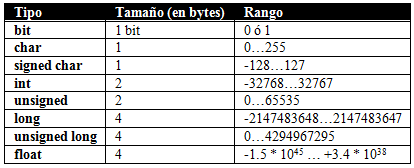
\includegraphics[scale=0.9]{TiposDatosC}
  \caption{Tipos de datos básicos utilizandos por el lenguaje c}
  \label{fig:tiposdatosc}
\end{figure}

De estos tipos de datos, los fundamentales son:
\begin{itemize}
\item Entero (int)
\item número de coma flotante (float).
\item caracteres (char).
\end{itemize}

char, int, float y double son palabras reservadas. Los tipos char, int y double tienen variaciones o modificadores de tipo de datos, tales como short, long, signed y unsigned, para permitir uso mas eficiente de los tipos de datos. \\

Un ejemplo de código en C++ que nos ayuda a comprender el uso del tipo de datos \textbf{float} es el que permite calcular las cuatro operaciones básicos (suma, resta, multiplicación y división).

\begin{lstlisting}[frame=trBL,firstnumber=1,caption={\textbf{OperBasi1.cpp}: Operaciones Básicas}]{Programa C++}
//======================================================
 Operaciones basicas (suma,resta,multiplica y divide
//======================================================
#include<iostream>
using namespace std;
int main()
{
  //para la suma de dos numeros.
  float x1=3,x2=5,x3=8,x4=11,x5=10,x6=9,x7=1,x8=2,s,r,m,d;


  s=x1+x2;   //Suma
  r=x3-x4;   //Resta
  m=x5*x6;   //Multiplicacion
 d=x7/x8;   //Division

  cout<<"El resultado de la suma fue: "<<s<<endl;
  cout<<"El resultado de la resta fue: "<<r<<endl;
  cout<<"El resultado de la multiplicacion fue: "<<m<<endl;
  cout<<"El resultado de la division fue: "<<d<<endl;

  return(0);
}
  
\end{lstlisting}

En esta porción de código además de aprender como declarar una variable de tipo float, también  aprendemos que a una variable podemos asignarle un valor utilizando una expresion de asignación.

    \begin{tcolorbox}[title=''Declaración de variable y Expresión de asignación'']
      $ float \; \;  X1=3; X2=5; $
    \end{tcolorbox}

    También podemos observar la utilización de cuatro expresiones matemáticas que utilizan los operadores matemáticos básicos como son la suma (+), la resta (-), la división (/) y la multiplicación (*).\\

    \begin{tcolorbox}[title=''Expresiones matemáticas'']
    $  s=x1+x2;  \;\; $               //suma\\
    $  r=x3-x4; \; \; $    //resta \\
    $  m=x5*x6; \;\; $     //multiplicación\\
    $  d=x7/x8; \;\; $    //división
    \end{tcolorbox}

    Este código aunque no presenta errores al momento de copilarlo, no tiene una aplicación real puesto que la asignación de los valores de las variables deben ser a criterio del usuario que va a utilizar el programa no del programador, y si asignamos los valores directamente en el código el unico que puede cambiarlo seria el programador a una persona que tenga conocimiento de programación y esto no estaria bien, es así en el siguiente código se soluciona este inconveniente utilizando la función \textbf{cin} y  \textbf{cout} para permitirle al usuario ingresar los valores que crea conveniente por teclado. 
\newpage
\begin{lstlisting}[frame=trBL,firstnumber=1,caption={\textbf{operbasi2.cpp}: Operaciones Básicas}]{Programa C++}
//======================================================
 Operaciones basicas (suma,resta,multiplica y divide)
//======================================================
#include<iostream>
using namespace std;
int main()
{
  //para la suma
  float x1,x2,s;
  // para la resta
  float x3,x4,r;
  // para la division
  float x5,x6,d;  
  // para la multiplicacion
  float x7,x9,d;
  
  cout<<"Ingrese los valores a sumar : ";
  cout<<"Ingrese x1 : ";cin>>x1;
  cout<<"Ingrese x2 : ";cin>>x2;

  cout<<"Ingrese los valores a sumar : ";
  cout<<"Ingrese x1 : ";cin>>x1;
  cout<<"Ingrese x2 : ";cin>>x2;

  cout<<"Ingrese los valores a sumar : ";
  cout<<"Ingrese x1 : ";cin>>x1;
  cout<<"Ingrese x2 : ";cin>>x2;

  cout<<"Ingrese los valores a sumar : ";
  cout<<"Ingrese x1 : ";cin>>x1;
  cout<<"Ingrese x2 : ";cin>>x2;

  s=x1+x2;
  r=x3-x4;
  m=x5*x6;
  d=x7/x8;

  cout<<"El resultado de la suma fue: "<<s<<endl;
  cout<<"El resultado de la resta fue: "<<r<<endl;
  cout<<"El resultado de la multiplicacion fue: "<<m<<endl;
  cout<<"El resultado de la division fue: "<<d<<endl;

  return(0);
}
  
\end{lstlisting}

    



    Aunque estas dos versiones del programas \textbf{OperBasi.cpp} funcionan,  estan muy lejos de satisfacer las necesidades de un usuario real, pues es dificil que alguien quiera rrealizar las cuatro operaciones matemáticas al mismo tiempo, esto no tiene sentido; lo que se si se aproxima a los requerimientos reales, es querer realizar una operacion a la vez y para eso debemos darle al usuario la opción de seleccionar que desea hacer:

\renewcommand\mylstcaption{\textbf{operbasi3.cpp}: Operaciones Básicas}

\begin{lstlisting}[frame=trBL,firstnumber=1,caption=\mylstcaption]{Programa C++}
//=======================================================
 Operaciones basicas (suma,resta,multiplica y divide)
//=======================================================
#include<iostream>
using namespace std;
int main()
{
  int op;
  float x1,x2,x3,x4,x5,x6,x7,x8,s,r,m,d;
  
  cout<<"Ingrese el numero de la operacion que quiere realizar : ";
  cout<<"1.- Suma : "<<endl;
  cout<<"2.- Resta :"<<endl;
  cout<<"3.- Producto :"<endl;
  cout<<"4.- Division:";

cout<<"Ingre la opcion: "; cin>>op;

 if(op==1){
  cout<<"Ingrese los valores a sumar : ";
  cout<<"Ingrese x1 : ";cin>>x1;
  cout<<"Ingrese x2 : ";cin>>x2;
  s=x1+x2;
  cout<<"El resultado de la suma fue: "<<s<<endl;
}
if (op==2){
  cout<<"Ingrese los valores a sumar : ";
  cout<<"Ingrese x1 : ";cin>>x1;
  cout<<"Ingrese x2 : ";cin>>x2;
  r=x3-x4;
  cout<<"El resultado de la resta fue: "<<r<<endl;
}
if(op==3){
  cout<<"Ingrese los valores a sumar : ";
  cout<<"Ingrese x1 : ";cin>>x1;
  cout<<"Ingrese x2 : ";cin>>x2;
  m=x5*x6;
  cout<<"El resultado de la multiplicacion fue: "<<m<<endl;
}
if(op==4){
  cout<<"Ingrese los valores a sumar : ";
  cout<<"Ingrese x1 : ";cin>>x1;
  cout<<"Ingrese x2 : ";cin>>x2;
  d=x7/x8;
  cout<<"El resultado de la division fue: "<<d<<endl;
}
  return(0);}
  
\end{lstlisting}



    Observamos que a medida que vamos mejorando el programa para que se adapte a las necesidades de un usuario real, el código se hace más extenso y más dificil de comprender, por ejemplo imagine que el usuario quiere que al seleccionar la opción de suma este le permita sumar varios números, o tiene la necesidad de sumar varios números positivos y varios número negativo y luego restar el resultado de los número positivos con el resultado de los número negativos; en la sección sobre diagrama de flujo ya se reviso este tipo de problema por lo que podemos deducir que el código para estos nuevos requerimientos seria dificil de leer; es por eso que se hace importante el uso de funciones.


\renewcommand\mylstcaption{\textbf{operbasi4.cpp}: Operaciones Básicas}
    
\begin{lstlisting}[frame=trBL,firstnumber=1,caption=\mylstcaption]{Programa C++}
//=======================================================
 Operaciones basicas(suma,resta,multiplica, divide)
//=======================================================
#include<iostream>
using namespace std;
int main()
{
  int op;
  float x1,x2,x3,x4,x5,x6,x7,x8,s,r,m,d;

do{
system("clear");  
  cout<<"Ingrese el numero de la operacion que quiere realizar : ";
  cout<<"1.- Suma : "<<endl;
  cout<<"2.- Resta :"<<endl;
  cout<<"3.- Producto :"<endl;
  cout<<"4.- Division:";
  cout<<"5.- Salir:";

cout<<"Ingre la opcion: "; cin>>op;

 if(op==1){
  cout<<"Ingrese los valores a sumar : ";
  cout<<"Ingrese x1 : ";cin>>x1;
  cout<<"Ingrese x2 : ";cin>>x2;
  s=x1+x2;
  cout<<"El resultado de la suma fue: "<<s<<endl;
}
if (op==2){
  cout<<"Ingrese los valores a sumar : ";
  cout<<"Ingrese x1 : ";cin>>x1;
  cout<<"Ingrese x2 : ";cin>>x2;
  r=x3-x4;
  cout<<"El resultado de la resta fue: "<<r<<endl;
}

if(op==3){
  cout<<"Ingrese los valores a sumar : ";
  cout<<"Ingrese x1 : ";cin>>x1;
  cout<<"Ingrese x2 : ";cin>>x2;
  m=x5*x6;
  cout<<"El resultado de la multiplicacion fue: "<<m<<endl;
}
if(op==4){
  cout<<"Ingrese los valores a sumar : ";
  cout<<"Ingrese x1 : ";cin>>x1;
  cout<<"Ingrese x2 : ";cin>>x2;
  d=x7/x8;
  cout<<"El resultado de la division fue: "<<d<<endl;
}

}while(op!=5);
  return(0);
}
  
\end{lstlisting}






\newgeometry{hmargin=2cm,vmargin=2cm,landscape}
\pdfpagewidth=297mm   %25in
\pdfpageheight=210mm %%16in
\textwidth=250mm
\textheight=190mm
\headwidth=\textwidth
\linewidth= 240mm
\begin{longtable}{|m{3cm}@{\hspace{0.4cm}}|m{2.3cm}|m{\linewidth-6cm}|}
 
  \hline
  \rowcolor{gray!20}
  Actividad                  & Criterio                      & Nivel 1          \\ \hline
 \hline 
\endfirsthead
  
  \multicolumn{3}{@{}l}{\ldots Continuación} \\ \hline \hline
  \rowcolor{gray!20}
  
  Actividad                  & Criterio                      & Nivel 1          \\ \hline

 \hline
 \endhead
\hline
  \multicolumn{3}{r@{}}{\ldots Continua  \ldots} \\ 
  \endfoot
  \hline
  \endlastfoot

\rowcolor{green!50}                                       
\multicolumn{2}{l|}{Nota máxima } & \makecell[r]{100} \\ \hline

                                        % ========================segundo parcial
  \multirow{3}{*}{ \actividadBB }        &\criterioBBA  & \nivelBBA  \\  \cline{2-3}
                                        & \criterioBBB & \nivelBBB   \\ \cline{2-3}
                                        & \criterioBBC & \nivelBBC   \\ \hline   
 \end{longtable}

\newpage
\begin{longtable}[H]{|b{0.5cm}|b{0.5cm}|b{0.5cm}|b{0.5cm}|b{0.5cm}|b{0.5cm}|b{10cm}|b{10cm}|}
\cabecera  

\multirow{3}{*}{\rotatebox{90}{DECIMA SEMANA}}  &  \multirow{3}{*}{\rotatebox[origin=c]{90}{01-noviembre-2021}}& \multirow{3}{*}{\rotatebox{90}{05-noviembre-2021}} &2&2&C& \multicolumn{2}{c|}{\semanaJA} \\ \cline{4-8}  
  &  &   &2& &C  & \multicolumn{2}{c|}{\semanaJB} \\ \cline{4-8} 
  &  &   &2& &C  & \multicolumn{2}{c|}{\semanaJC} \\ \hline

  
\end{longtable}

\newpage
\restoregeometry

\subsubsection{Estructura de selección (if-else) en C++}
\label{sec:estr-de-selecc}



    \begin{tcolorbox}[title=''Sintaxis estructura if'']
      if(<operación\_lógica>)\\
      \{\\
        instrucione1;\\
        instruccion2;\\
        ......\\
        insruccion\_n;\\
        \}\\
        else\\
        \{\\
        instrucione1;\\
        instruccion2;\\
        ......\\
        insruccion\_n;\\
        \}\\
    \end{tcolorbox}



\begin{tcolorbox}[skin=widget,
boxrule=1mm,
coltitle=black,
colframe=blue!45!white,colback=blue!15!white,width=(1\linewidth),before=\hfill,after=\hfill,adjusted title={\textbf{Preguntas para el autocontrol}}]
Estan agrupadas por fases.  
\tcblower

\begin{itemize}
\item \textbf{Pregunta \# 1:} A quien se le atribuje la arquitectura del computador.
  \begin{itemize}
  \item  char babage.
  \item Jhon Vom Neumann.
  \item Rober Noise.
  \end{itemize}
\item \textbf{fase \# 2:} Dar seguimiento al proceso académico de las asignaturas.
  \begin{itemize}
  \item Llevar el control de asistencia tanto de maestrantes como de docentes.
  \item Manejar toda la información que genera el proceso académico (silabos, módulos, tareas, etc.)
  \item Control de cumplimiento de actividades de acuerdo a un cronograma.
  \item Ingreso y difusión de calificaciones.
  \end{itemize}
\item \textbf{fase \# 3:} Gestionar la información académica.
  \begin{itemize}
  \item Repositorio digital.
  \item Control de carga y descarga de información al Repositorio.
  \item Busqueda de información. 
  \end{itemize}
\item \textbf{fase \# 4:} Manejar la relación con los maestrantes y docente.
  \begin{itemize}
  \item Integración con Microsoft Team y Google ClassRoom.
  \item Integración con Microsoft Team y Google ClassRoom.
  \item Integración con Microsoft Team y Google ClassRoom.
  \end{itemize}
\end{itemize}

\end{tcolorbox}


\newgeometry{hmargin=2cm,vmargin=2cm,landscape}
\pdfpagewidth=297mm   %25in
\pdfpageheight=210mm %%16in
\textwidth=250mm
\textheight=190mm
\headwidth=\textwidth
\linewidth= 240mm

\begin{longtable}{|m{3cm}@{\hspace{0.4cm}}|m{2.3cm}|m{\linewidth-6cm}|}
 
  \hline
  \rowcolor{gray!20}
  Actividad                  & Criterio                      & Nivel 1          \\ \hline
 \hline 
\endfirsthead
  
  \multicolumn{3}{@{}l}{\ldots Continuación} \\ \hline \hline
  \rowcolor{gray!20}
  
  Actividad                  & Criterio                      & Nivel 1          \\ \hline

 \hline
 \endhead
\hline
  \multicolumn{3}{r@{}}{\ldots Continua  \ldots} \\ 
  \endfoot
  \hline
  \endlastfoot

\rowcolor{green!50}                                       
\multicolumn{2}{l|}{Nota máxima } & \makecell[r]{100} \\ \hline

\multirow{3}{*}{ \actividadCB }        &\criterioCBA  & \nivelCBA  \\  \cline{2-3}
                                        & \criterioCBB & \nivelCBB   \\ \cline{2-3}
                                        & \criterioCBC & \nivelCBC   \\ \hline   


\end{longtable}

\newpage
\begin{longtable}[H]{|b{0.5cm}|b{0.5cm}|b{0.5cm}|b{0.5cm}|b{0.5cm}|b{0.5cm}|b{10cm}|b{10cm}|}

\cabecera


\multirow{3}{*}{\rotatebox{90}{ONCEVA SEMANA}}  &  \multirow{3}{*}{\rotatebox[origin=c]{90}{08-nobiembre-2021}}& \multirow{3}{*}{\rotatebox{90}{12-noviembre-2021}} &2&0&C& \multicolumn{2}{c|}{\semanaKA} \\ \cline{4-8}  
  &  &   &2&0&C  & \multicolumn{2}{c|}{\semanaKB} \\ \cline{4-8}  
  &  &   &2&0&C  & \multicolumn{2}{c|}{\semanaKC} \\ \hline

\end{longtable}

\newpage
\restoregeometry

\subsubsection{Estructura de repetición (do-while)
}


En esta porción de se utiliza hay que aplicar el  bucle o lazo de repeticion ( do{.....}while), cuya sintaxis es la siguiente:

    \begin{tcolorbox}[title=''Sintaxis de un do{...}while(..);'']
      do\{\\
        instrucione1;\\
        instruccion2;\\
        ......\\
        insruccion\_n;\\
       \}while(<operacion lógica>);
    \end{tcolorbox}

    \newpage
\subsubsection{Taller para estructura de repetición}

     Otro ejemplo de que las funciones evolucionan y se hacen más grandes y complejas es la función de la división que se lo puede interpretar como el resultado de una fracción y se puede extender la función para que devuelva el resultado de la suma de varias fracciones.

    \begin{lstlisting}[frame=trBL,caption={\textbf{sumafracciones()}}]{Programa C++,title=''Practica 1''}
  #include<iostream>
  using namespace std;
  int main()
  {
   int i=0,s=0,cposi=0,cnega=0,sposi=0,snega=0;
   float x;
   cout<< ``Ingresa la cantidad de fracciones:'';
   cin>>cf;
   do{
   cout<< ``Ingresa el numerador:'';   cin>>n;
   cout<< ``Ingresa el denominador:'';   cin>>d;
   i=i+1;
   cociente=cociente+n/d;
  cout<<n<<"/"<<d<<"+";
  }while(i<cf);
   cout<<"= "<<s<< endl;
   return 0;
  }
\end{lstlisting}




\begin{tcolorbox}[skin=widget,
boxrule=1mm,
coltitle=black,
colframe=blue!45!white,colback=blue!15!white,width=(1\linewidth),before=\hfill,after=\hfill,adjusted title={\textbf{Preguntas para el autocontrol}}]
Estan agrupadas por fases.  
\tcblower

\begin{itemize}
\item \textbf{Pregunta \# 1:} A quien se le atribuje la arquitectura del computador.
  \begin{itemize}
  \item  char babage.
  \item Jhon Vom Neumann.
  \item Rober Noise.
  \end{itemize}
\item \textbf{fase \# 2:} Dar seguimiento al proceso académico de las asignaturas.
  \begin{itemize}
  \item Llevar el control de asistencia tanto de maestrantes como de docentes.
  \item Manejar toda la información que genera el proceso académico (silabos, módulos, tareas, etc.)
  \item Control de cumplimiento de actividades de acuerdo a un cronograma.
  \item Ingreso y difusión de calificaciones.
  \end{itemize}
\item \textbf{fase \# 3:} Gestionar la información académica.
  \begin{itemize}
  \item Repositorio digital.
  \item Control de carga y descarga de información al Repositorio.
  \item Busqueda de información. 
  \end{itemize}
\item \textbf{fase \# 4:} Manejar la relación con los maestrantes y docente.
  \begin{itemize}
  \item Integración con Microsoft Team y Google ClassRoom.
  \item Integración con Microsoft Team y Google ClassRoom.
  \item Integración con Microsoft Team y Google ClassRoom.
  \end{itemize}
\end{itemize}

\end{tcolorbox}

\newgeometry{hmargin=2cm,vmargin=2cm,landscape}
\pdfpagewidth=297mm   %25in
\pdfpageheight=210mm %%16in
\textwidth=250mm
\textheight=190mm
\headwidth=\textwidth
\linewidth= 240mm

\newpage
\begin{longtable}[H]{|b{0.5cm}|b{0.5cm}|b{0.5cm}|b{0.5cm}|b{0.5cm}|b{0.5cm}|b{10cm}|b{10cm}|}
\cabecera  

 \multirow{3}{*}[-10ex]{\rotatebox{90}{DOCEAVA SEMANA}}  & \multirow{3}{*}[-10ex]{\rotatebox[origin=c]{90}{15-noviembre-2021}}& \multirow{3}{*}[-10ex]{\rotatebox{90}{19-noviembre-2021}} &2&0&C& \multicolumn{2}{c|}{\semanaLA} \\ \cline{4-8}  
  &  &   &2&0&C  & \multicolumn{2}{c|}{\semanaLB} \\ \cline{4-8}   
  &  &   &2&0&C  & \multicolumn{2}{c|}{\semanaLC} \\ \hline


\end{longtable}

\newpage
\restoregeometry

\subsubsection{Proyecto Final Integrador }







    \begin{tcolorbox}[title=''Sentencia switch'']
      switch(<identificador de variable>) \{\\
        case <valor de la variable>;\\
        sentencias;\\
        ..........;\\
        case <valor de la variable>;\\
        sentencias;\\
        ..........;\\
        case <valor de la variabla>;\\
        ......\\
        default;\\
       \}
    \end{tcolorbox}
Como vimos en el programa \textbf{OperBasi5.cpp} se necesito utilizar varias estructuras \textbf{if} para seleccionar que operacion el usuario desea ejecutar, esa implementación puede resultar poco efeciente puesto que si el usuario desea ejecuta una solo opción, el progama evaluará todas las opeciones utilizando el CPU innecesariamente,  es por eso que una mejor opción para implementar un menú es mediante la estructura \textbf{swith-case} presentada en el recuadro anterior.

\newpage
    Implementando el programa \textbf{OperBasi5.cpp} con la estructura \textbf{case} el nuevo programa queradaria de la siguiente manera:

    \renewcommand\mylstcaption{\textbf{OperBAsi6.cpp}}

\begin{lstlisting}[frame=trBL,caption=\mylstcaption]{Programa C++,title=''Practica 1''}
  #include<iostream>
  using namespace std;
  int main()
  {
   int i=0,s=0;
   float x;
   do{

   switch{op}
   {
   case 1:
     suma(); 
   breack;
   case 2:
     resta();
     break();
   case 3:
     divide();
     break;
   case 4:
     producto();
     breack;
   case 5:
      break;
   }
   i=i+1;
   s=s+x;
  }while(op != 5);
   cout<<"La suma fue: "<<s<< endl;
   return 0;
  }
\end{lstlisting}
\vfill


\begin{tcolorbox}[skin=widget,
boxrule=1mm,
coltitle=black,
colframe=blue!45!white,colback=blue!15!white,width=(1\linewidth),before=\hfill,after=\hfill,adjusted title={\textbf{Preguntas para el autocontrol}}]
Estan agrupadas por fases.  
\tcblower

\begin{itemize}
\item \textbf{Pregunta \# 1:} A quien se le atribuje la arquitectura del computador.
  \begin{itemize}
  \item  char babage.
  \item Jhon Vom Neumann.
  \item Rober Noise.
  \end{itemize}
\item \textbf{fase \# 2:} Dar seguimiento al proceso académico de las asignaturas.
  \begin{itemize}
  \item Llevar el control de asistencia tanto de maestrantes como de docentes.
  \item Manejar toda la información que genera el proceso académico (silabos, módulos, tareas, etc.)
  \item Control de cumplimiento de actividades de acuerdo a un cronograma.
  \item Ingreso y difusión de calificaciones.
  \end{itemize}
\item \textbf{fase \# 3:} Gestionar la información académica.
  \begin{itemize}
  \item Repositorio digital.
  \item Control de carga y descarga de información al Repositorio.
  \item Busqueda de información. 
  \end{itemize}
\item \textbf{fase \# 4:} Manejar la relación con los maestrantes y docente.
  \begin{itemize}
  \item Integración con Microsoft Team y Google ClassRoom.
  \item Integración con Microsoft Team y Google ClassRoom.
  \item Integración con Microsoft Team y Google ClassRoom.
  \end{itemize}
\end{itemize}

\end{tcolorbox}


\newgeometry{hmargin=2cm,vmargin=2cm,landscape}
\pdfpagewidth=297mm   %25in
\pdfpageheight=210mm %%16in
\textwidth=250mm
\textheight=190mm
\headwidth=\textwidth
\linewidth= 240mm

\begin{longtable}{|m{3cm}@{\hspace{0.4cm}}|m{2.3cm}|m{\linewidth-6cm}|}
 
  \hline
  \rowcolor{gray!20}
  Actividad                  & Criterio                      & Nivel 1          \\ \hline
 \hline 
\endfirsthead
  
  \multicolumn{3}{@{}l}{\ldots Continuación} \\ \hline \hline
  \rowcolor{gray!20}
  
  Actividad                  & Criterio                      & Nivel 1          \\ \hline

 \hline
 \endhead
\hline
  \multicolumn{3}{r@{}}{\ldots Continua  \ldots} \\ 
  \endfoot
  \hline
  \endlastfoot

\rowcolor{green!50}                                       
\multicolumn{2}{l|}{Nota máxima } & \makecell[r]{100} \\ \hline
  \multirow{3}{*}{ \actividadAB }        &\criterioABA  & \nivelABA  \\  \cline{2-3}
                                        & \criterioABB & \nivelABB   \\ \cline{2-3}
                                        & \criterioABC & \nivelABC   \\ \hline   

\multicolumn{2}{l|}{Nota máxima } & \makecell[r]{100} \\ \hline
  




\end{longtable}



\newpage
\begin{longtable}[H]{|b{0.5cm}|b{0.5cm}|b{0.5cm}|b{0.5cm}|b{0.5cm}|b{0.5cm}|b{10cm}|b{10cm}|}
\cabecera
  \multirow{3}{*}[-10ex]{\rotatebox{90}{TRECEAVA SEMANA}}  & \multirow{3}{*}[-10ex]{\rotatebox[origin=c]{90}{22-noviembre-2021}}& \multirow{3}{*}[-10ex]{\rotatebox{90}{26-noviembre-2021}} &2& &C& \multicolumn{2}{c|}{\semanaMA} \\ \cline{4-8}
  &  &   &2& &C  & \multicolumn{2}{c|}{\semanaMB} \\ \cline{4-8}    
  &  &   &2& &C  & \multicolumn{2}{c|}{\semanaMC} \\ \hline

\end{longtable}

\newpage
\restoregeometry




\begin{tcolorbox}[skin=widget,
boxrule=1mm,
coltitle=black,
colframe=blue!45!white,colback=blue!15!white,width=(1\linewidth),before=\hfill,after=\hfill,adjusted title={\textbf{Preguntas para el autocontrol}}]
Estan agrupadas por fases.  
\tcblower

\begin{itemize}
\item \textbf{Pregunta \# 1:} A quien se le atribuje la arquitectura del computador.
  \begin{itemize}
  \item  char babage.
  \item Jhon Vom Neumann.
  \item Rober Noise.
  \end{itemize}
\item \textbf{fase \# 2:} Dar seguimiento al proceso académico de las asignaturas.
  \begin{itemize}
  \item Llevar el control de asistencia tanto de maestrantes como de docentes.
  \item Manejar toda la información que genera el proceso académico (silabos, módulos, tareas, etc.)
  \item Control de cumplimiento de actividades de acuerdo a un cronograma.
  \item Ingreso y difusión de calificaciones.
  \end{itemize}
\item \textbf{fase \# 3:} Gestionar la información académica.
  \begin{itemize}
  \item Repositorio digital.
  \item Control de carga y descarga de información al Repositorio.
  \item Busqueda de información. 
  \end{itemize}
\item \textbf{fase \# 4:} Manejar la relación con los maestrantes y docente.
  \begin{itemize}
  \item Integración con Microsoft Team y Google ClassRoom.
  \item Integración con Microsoft Team y Google ClassRoom.
  \item Integración con Microsoft Team y Google ClassRoom.
  \end{itemize}
\end{itemize}

\end{tcolorbox}


\newgeometry{hmargin=2cm,vmargin=2cm,landscape}
\pdfpagewidth=297mm   %25in
\pdfpageheight=210mm %%16in
\textwidth=250mm
\textheight=190mm
\headwidth=\textwidth
\linewidth= 240mm

\newpage
\begin{longtable}[H]{|b{0.5cm}|b{0.5cm}|b{0.5cm}|b{0.5cm}|b{0.5cm}|b{0.5cm}|b{10cm}|b{10cm}|}
\cabecera  

  \multirow{3}{*}[-10ex]{\rotatebox{90}{CATORCEAVA SEMANA}}  &  \multirow{3}{*}[-10ex]{\rotatebox[origin=c]{90}{29-noviembre-2021}}& \multirow{3}{*}[-10ex]{\rotatebox{90}{03-diciembre-2021}} & 2& &C& \multicolumn{2}{c|}{\semanaNA} \\ \cline{4-8}   
  &  &   &2& &C & \multicolumn{2}{c|}{\semanaNB} \\ \cline{4-8}   
  &  &   &2& &C  & \multicolumn{2}{c|}{\semanaNC} \\ \hline

\end{longtable}

\newpage
\restoregeometry


\section{Funciones declaradas por el usuario}
\label{sec:funciones}

Como pudimos observar en la evolución del código anterior, a medida que el programa se hace más real, en el sentido de poder ser usable en un ambiente real,  su complejidad funcional aumenta, y mantener todas las lineas de código en un mismo archivo no resulta conveniente para poder seguir actualizandolo, pues demasiadas lineas de código lo convierte en un documento dificil de leer. Es por eso que se hace necesario crear unidades funcionales más pequeñas, es decir su funcionalidad dividirlas en archivos que contengan solo las lineas de código relacionadas a traves de la función que estas realicen.\\

El siguiente recuadro presenta la sintaxis que debe ser usada para crear una función 
    \begin{tcolorbox}[title=''Sintaxis de un función'']
      <tipo datos><indentificador\_de\_funcion>(<para\_1>...<para\_n>)\\
      \{\\
        instruccion\_1;\\
        instruccion\_2;\\
        ......\\
        ......\\
        instruccion\_n;\\
        return <identificador\_de\_variable>;\\
       \}
    \end{tcolorbox}
Podemos resaltar que una función declarada por el usuario, tiene la misma estructura que la función principal\textbf{ main}, es decir devuelve un tipo de datos y recibe parametros declarados de cualquier tipo; pero estas funciones creados por el usuario/programador,  deben ser declaradas antes de la función principal main que es de donde por lo general se las llama.
    
En los siguientes ejemplos se muestran cuatro funciones (suma(), resta(), producto() y division()), y luego se implementa una función principal \textbf{main} de donde se las llama, se espera que estos ejemplos permitan su mejor comprención.\\

\newpage

Función suma : Suma dos números pasasos como argumento.

\renewcommand\mylstcaption{\textbf{suma.cpp}: función suma}

\begin{lstlisting}[frame=trBL,firstnumber=1,caption=\mylstcaption]{Programa C++}
//==============================================
// Funcion suma
//==============================================
#include<iostream>
using namespace std;
float suma(float x1,float x2)
{
return(x+y);
}
\end{lstlisting}

Podemos colocar la función resta en otro archivo

\begin{lstlisting}[frame=trBL,firstnumber=1,caption={\textbf{resta.cpp}: funcion resta}]{Programa C++}
//==============================================
// Funcion resta
//==============================================
#include<iostream>
using namespace std;
float resta(float x1,float x2)
{
return(x-y);
}
\end{lstlisting}

\newpage
El archivo para la función producto.\\

    \begin{lstlisting}[frame=trBL,firstnumber=0,caption={\textbf{producto.cpp}: función producto}]{Programa C++}
//=============================================
// Funcion producto
//=============================================
#include<iostream>
using namespace std;
float producto(float x1,float x2)
{
return(x*y);
}
\end{lstlisting}
\newpage
Creamos un archivo llamado division.cpp para escribir la función divide que devide dos números.\\
    \begin{lstlisting}[frame=trBL,firstnumber=0,caption={\textbf{division.cpp}: Operaciones Básicas}]{Programa C++}
//=============================================
// Funcion division
//=============================================
#include<iostream>
using namespace std;
float divide(float x1,float x2)
{
return(x1/x2);
}
\end{lstlisting}

Para poder utilizar estos archivos que contienen la funciones de suma(), resta(), producto() y division() es necesario utilizar las directivas que cargan los archivos junto con el programa principal de la siguiente manera:

\renewcommand\mylstcaption{\textbf{OperBasi5.cpp}: función suma}

\begin{lstlisting}[frame=trBL,firstnumber=1,caption={\textbf{OperBasi5.cpp}}]{Programa C++}
//==============================================
// Operaciones Basica Recargada
//==============================================
#include<iostream>
#include "suma.cpp"
#include "resta.cpp"
#include "producto.cpp"
#include "divide.cpp"

using namespace std;
int main()
{
float x,y;

cout<<"ingre el numero de la opracion que desa realizar";
cout << "1=suma"<<endl;
cout << "2=resta"<<endl;
cout << "3=producto"<<endl;
cout << "4=division"<<endl;
cin>>opc;

if(opc==1){
   cout<<"Ingrese el primer sumando: "; cin<<x;
   cout<<"Ingrese el segundo sumando: "; cin<<y;
   cout<<"El suma dio:"<<suma(x,y)<<endl;
}

if(opc==2){
   cout<<"Ingrese el minuendo: "; cin<<x;
   cout<<"Ingrese el sustraendo:"; cin<<y;
   cout<<"El resta dio: "<<resta(x,y)<<endl;
}
if(opc==3){
   cout<<"Ingrese el primer factor: "; cin<<x;
   cout<<"Ingrese el segundo factor:"; cin<<y;
   cout<<"El multiplicacion dio:"<<producto(x,y)<<endl;
}
if(opc==4){
   cout<<"Ingrese el dividendo: "; cin<<x;
   cout<<"Ingrese el divisor:"; cin<<y;
   cout<<"El division dio :"<<divide(x,y)<<endl;}
}
\end{lstlisting}

Utilizar funciones es importente por que esto permite concentrar el esfuerzo que se realiza en la etapa de la actualización, en  una parte del código, por ejemplo, si deseamos que la suma sea de varios número solo tenemos que modificar el archivo de suma.cpp y reemplazar esta porción de código. \\

\renewcommand\mylstcaption{\textbf{sumanúmeros.cpp}: función suma}

\begin{lstlisting}[frame=trBL,caption={\textbf{sumanúmeros()}}]{Programa C++,title=''Practica 1''}
  #include<iostream>
  using namespace std;
  int main()
  {
   int i=0,s=0,cposi=0,cnega=0,sposi=0,snega=0;
   float x;
   do{
   cout<< ``Ingresa un numero entero:''; cin>>x;
   i=i+1;
   s=s+x;
   if(x>0){
    cposi=cposi+1;   sposi=sposi+x;
   } else {
    cnega=cnega+1;   snega=snega+x;
   }
  }while(i<10);
   cout<<"La suma fue: "<<s<< endl;
   return 0;
  }
\end{lstlisting}


\subsection{Clases: Estructura}
\label{sec:clases}

Una característica que identifica al lenguaje C++ es la programación orientada a objetos, esto significa que se pueden utilizar estructuras llamadas clases, las cuales permiten agrupar atributos y eventos o funciones de un objeto para ser utilizados como una sola unidad lógica.\\

En C++ los atributos reciben el nombre de datos miembros y los métodos el nombre de funciones miembros de la clases incluyento los miembros constructures que permiten inicializar un obejeto y los destructores que permiten destruir un objeto~\cite{sierra98}.\\

De forma general la estructura clases es:



    \begin{tcolorbox}[title=''estructura de datos CLASS'']
      class <Identificador de la clase> \{\\
        public;\\
        <tipo de datos> <identificador de variable>;\\
        ..........;\\
        protected:\\
        <tipo de datos> <identificador de variable>;\\

        private:\\
        <tipo de datos> <identificador de variable>;\\

        ..........;\\
        case <valor de la variabla>;\\

        
        ..........;\\
        case <valor de la variabla>;\\
        ......\\
        ......\\
;\\
       \}\\
    \end{tcolorbox}
\newpage
  Un ejemplo de clase bastante utilizado, es la clase persona que en C++ se implementa de la siguiente manera:
    
\renewcommand\mylstcaption{\textbf{Persona.cpp}}

\begin{lstlisting}[frame=trBL,breaklines=true, firstnumber=1,caption=\mylstcaption]{Programa C++,title=''Practica 1''}

// Clase base Persona:
class Persona {
  public:
   Persona(char *n, int e);
   const char *LeerNombre(char *n) const;
   int LeerEdad() const;
   void CambiarNombre(const char *n);
   void CambiarEdad(int e);
   
  protected:
   char nombre[40];
   int edad;
};
 
// Clase derivada Empleado:
int main()
{  
   Persona person;
};
\end{lstlisting}

\newpage

\subsection{Preguntas de autocontrol}
\label{sec:preg-de-autoc-4}

\begin{itemize}
\item \textbf{Pregunta \# 1:} A quien se le atribuje la arquitectura del computador.
  \begin{itemize}
  \item  char babage.
  \item Jhon Vom Neumann.
  \item Rober Noise.
  \end{itemize}
\item \textbf{fase \# 2:} Dar seguimiento al proceso académico de las asignaturas.
  \begin{itemize}
  \item Llevar el control de asistencia tanto de maestrantes como de docentes.
  \item Manejar toda la información que genera el proceso académico (silabos, módulos, tareas, etc.)
  \item Control de cumplimiento de actividades de acuerdo a un cronograma.
  \item Ingreso y difusión de calificaciones.
  \end{itemize}
\item \textbf{fase \# 3:} Gestionar la información académica.
  \begin{itemize}
  \item Repositorio digital.
  \item Control de carga y descarga de información al Repositorio.
  \item Busqueda de información. 
  \end{itemize}
\item \textbf{fase \# 4:} Manejar la relación con los maestrantes y docente.
  \begin{itemize}
  \item Integración con Microsoft Team y Google ClassRoom.
  \item Integración con Microsoft Team y Google ClassRoom.
  \item Integración con Microsoft Team y Google ClassRoom.
  \end{itemize}
\end{itemize}



\newgeometry{hmargin=2cm,vmargin=2cm,landscape}
\pdfpagewidth=297mm   %25in
\pdfpageheight=210mm %%16in
\textwidth=250mm
\textheight=190mm
\headwidth=\textwidth
\linewidth= 240mm

\newpage
\begin{longtable}[H]{|b{0.5cm}|b{0.5cm}|b{0.5cm}|b{0.5cm}|b{0.5cm}|b{0.5cm}|b{10cm}|b{10cm}|}
\cabecera

 \multirow{3}{*}[-10ex]{\rotatebox{90}{QUINCEAVA SEMANA}} & \multirow{3}{*}[-10ex]{\rotatebox[origin=c]{90}{06-diciembre-2021}}& \multirow{3}{*}[-10ex]{\rotatebox{90}{10-diciembre-2021}} &2& &C& \multicolumn{2}{c|}{\semanaOA} \\ \cline{4-8}   
  &  &   &2& &C  & \multicolumn{2}{c|}{\semanaOB} \\ \cline{4-8} 
  &  &   &2& &C  & \multicolumn{2}{c|}{\semanaOC} \\ \hline

 
\end{longtable}

\newpage
\restoregeometry



\newgeometry{hmargin=2cm,vmargin=2cm,landscape}
\pdfpagewidth=297mm   %25in
\pdfpageheight=210mm %%16in
\textwidth=250mm
\textheight=190mm
\headwidth=\textwidth
\linewidth= 240mm

\newpage
\begin{longtable}[H]{|b{0.5cm}|b{0.5cm}|b{0.5cm}|b{0.5cm}|b{0.5cm}|b{0.5cm}|b{10cm}|b{10cm}|}
\cabecera
  \multirow{3}{*}[-10ex]{\rotatebox{90}{DIECISEISAVA SEMANA}}  & \multirow{3}{*}[-10ex]{\rotatebox[origin=c]{90}{13-diciembre-2021}}& \multirow{3}{*}[-10ex]{\rotatebox{90}{17-diciembre-2021}} &2& &C& \multicolumn{2}{c|}{\semanaPA} \\ \cline{4-8}   
  &  &   &2& &C  & \multicolumn{2}{c|}{\semanaPB} \\ \cline{4-8}   
  &  &   &2& &C  & \multicolumn{2}{c|}{\semanaPC} \\ \hline
  
\end{longtable}

%\endgroup

\newpage

\begin{center}
\begin{tabular}{|l|l|l|p{10cm}|}
  \hline
  \rowcolor{gray!20}
Semana &  Desde & hasta & Actividad\\
\hline \rowcolor{yellow!20}
       &    23-agosto-2021 & 27-agosto-2021 & Entrega de guía de estudio a dirección de carrera \\ \hline \rowcolor{yellow!20}
       &    30-agosto-2021 & 03-septiembre-2021 & Entrega y subida de silabo \\ \hline \rowcolor{blue!20}
 \multicolumn{4}{|c|}{INICIO PRIMER PARCIAL} \\ \hline \rowcolor{green!20}    
Semena \#1 & 30-agosto-2021 & 03-noviembre-2021 & Clases  - Presentación del Docente\\ \rowcolor{green!20}   
Semena \#2 & 06-septiembre-2021 & 10-noviembre-2021 & Clases - Envio de primera actividad(B1)\\ \rowcolor{green!20}
Semena \#3 & 13-septiembre-2021 & 17-noviembre-2021 & Clases - Entrega de calificación B1 \\   \rowcolor{green!20}
Semana \#4 & 20-septiembre-2021 & 24-noviembre-2021 & Clases - Envia de Actividad (C1)\\  \rowcolor{green!20}
Semana \#5 & 27-septiembre-2021 & 27-noviembre-2021 & Clases - Entrega de calificaciones  C1\\ \rowcolor{green!20}
Semana \#6 & 04-octubre-2021 & 08-octubre-2021 & Clases - Envia de Actividad (A1 Anteproyecto) \\  \rowcolor{green!20}
Semana \#7 & 11-octubre-2021 & 15-octubre-2021 & Clases - Entrega de calificación A1  \\ \rowcolor{green!20}
  Semana \#8 & 18-octubre-2021 & 22-octubre-2021 & EVALUACION SUMATIVA PRIMER PARCIAL\\ \hline \rowcolor{blue!20}
 \multicolumn{4}{|c|}{INICIO SEGUNDO PARCIAL} \\ \hline \rowcolor{green!20}
Semana \#9 & 25-octubre-2021 & 29-octubre-2020 & Clases - Envio de actividad B2\\ \rowcolor{green!20} 
Semana \#10  & 01-noviembre-2021 & 05-noviembre-2021 & Clases Entrega de calificación B2\\ \rowcolor{green!20}
Semana \#11 &  08-noviembre-2021 & 12-noviembre-2021 & Clases - Envio de actividad C2 \\ \rowcolor{green!20}
Semana \#12 &  15-noviembre-2021 & 19-noviembre-2021 & Clases - Entrega de calificacion C2\\   \rowcolor{green!20}
Semana \#13 &  22-noviembre-2021 & 26-noviembre-2021 & Clases - Envio de Actividad (A2 -Proyecto final)\\ \rowcolor{green!20}
Semana \#14 &  29-noviembre-2021 & 03-diciembre-2021 & Clases - Entraga calificación A2\\ \rowcolor{red!20}
Semana \#15 &  06-diciembre-2021 & 10-diciembre-2021 & EVALUACION SUMATIVA FINAL\\ \hline \rowcolor{red!20}
Semana \#16 &  13-diciembre-2021 & 17-diciembre-2021 & Evaluación de habilitación\\ \hline
\end{tabular}
\end{center}





\restoregeometry

\subsection{Formas y tipos de evaluación}
\label{sec:formas-y-tipos}

\begin{tabular}[H]{|m{4cm}|m{5cm}|m{4cm}|r|r|}
  \hline \hline
  EVALUACION & TIPOS & OPCIONES & PTOS. & $\sum$ \\ \hline \hline
   \multirow{4}{*}{Medio Ciclo} & \multirow{3}{*}{Acumulativa 70\%} & Actividad A1 & 3.5 \\ \cline{3-3}
             &                                    & Actividad B1 & 1.75 \\ \cline{3-3}
             &                                    & Actividad C1 & 1.75\\ \cline{2-3}
             &Examen medio ciclo 30\% & Evaluación sumativa &3 \\ \hline \hline
  \multicolumn{4}{r}{SUBTOTAL:} & 10 \\ \hline
   \multirow{4}{*}{Fin de Ciclo} & \multirow{3}{*}{Acumulativa 70\%} & Actividad A1 & 3.5 \\ \cline{3-3}
             &                                    & Actividad B1 & 1.75 \\ \cline{3-3}
             &                                    & Actividad C1 & 1.75\\ \cline{2-3}
             &Examen final 30\% & Evaluación sumativa &3 \\ \hline \hline
  \multicolumn{4}{r}{SUBTOTAL:} & 10 \\ \hline
  \multicolumn{4}{r}{PROMEDIO:} & 10 \\ \hline

  
\end{tabular}

\vspace{0.3cm}
\begin{center}
\begin{tabular}[H]{lll}
  \rule{5cm}{0.4pt}&  &\rule{5cm}{0.4pt} \\
  \makecell[l]{Ing. Stalin Francis Ms.c\\\textbf{ DOCENTE}}  & &\makecell[l]{Ing. Stalin Francis MSc. \\ \textbf{COORDINADOR DE ÁREA ACADÉMICA} \\ \textbf{DE PROGRAMACIÓN}} \\ 


  \rule{7cm}{0.4pt}&  &\rule{5cm}{0.4pt} \\
  \makecell[l]{Ing. Baster Estupiñan Ortiz, MSc. \\ \textbf{DIRECTOR DE CARRERA DE INGENIERÍA} \\ \textbf{EN TECNOLOGÍÁ DE LA INFORMACIÓN}} & & \makecell[l]{Ing. Fabiola Espantoso \\ \textbf{SECRETARIA}} 
\end{tabular}
\end{center}





\subsection{Rubricas para autoevaluación del silabo}
\label{sec:rubr-para-aprob}

\begin{center}
\renewcommand{\arraystretch}{1}%
\begin{tabular}[H]{|l|l|l|}
  \hline
\rowcolor{gray!50}

 \textcolor{white}{\textbf{CRITERIO}}  & \textcolor{white}{\textbf{SI}} & \textcolor{white}{\textbf{NO}} \\ \hline \hline
\rowcolor{green!20}
  \multicolumn{3}{l}{\textbf{DESCRIPCIÓN DE LA ASIGNATURA}} \\ \hline \hline

  Los datos informativos esta completos: & {\Large $\square$} &{\Large $\square$} \\ \hline
  La descripción de la asignatura es clara: &{\Large $\square$}  &{\Large $\square$} \\ \hline
  El Objetivo General es claro:&{\Large $\square$}  &{\Large $\square$} \\ \hline
  Los resultados de aprendizaje son claros(1 por cada unidad) &{\Large $\square$} &{\Large $\square$} \\ \hline 
  Se indica la metodología de aprendizaje(Aula invertida, otros) &{\Large $\square$} &{\Large $\square$} \\ \hline 
  Se indica los contenidos (Unidades y tema)  &{\Large $\square$} &{\Large $\square$} \\ \hline
  Estan definidas las 6 actividades (A1,B1,C1,A2,B2,C2) &{\Large $\square$} &{\Large $\square$} \\ \hline
  Estan definidas las 3 evaluaciones( E1, E1,R(Recuperacion)) &{\Large $\square$} &{\Large $\square$} \\ \hline \hline
  \rowcolor{green!20}
  \multicolumn{3}{l}{\textbf{GESTIÓN DURACIÓN DE ESTUDIO}} \\ \hline \hline
  Estan definidas las 16 semanas de clases &{\Large $\square$} &{\Large $\square$} \\ \hline
  Estan defindos los días y horas de cada \textbf{clases `` virtual''} &{\Large $\square$} &{\Large $\square$} \\ \hline
  Estan definidas las \textbf{actividades autónomas} y su duración &{\Large $\square$} &{\Large $\square$} \\ \hline
  Estan definidas las fechas y horas de \textbf{tutorias} &{\Large $\square$} &{\Large $\square$} \\ \hline \hline
  \rowcolor{green!20}
  \multicolumn{3}{l}{\textbf{GETIÓN INTERACCIÓN DOCENTE-ESTUDIANTE}} \\ \hline \hline
 Estan definidos los temas para cada clase ``virtual'' &{\Large $\square$} &{\Large $\square$} \\ \hline
  Esta definido el orden del día para las clases virtuales  &{\Large $\square$} &{\Large $\square$} \\ \hline
  Esta definido el tema para cada tutoria   &{\Large $\square$} &{\Large $\square$} \\ \hline \hline
    \rowcolor{green!20}
  \multicolumn{3}{l}{\textbf{BIBLIOGRAFÍA}} \\ \hline \hline
  
  Esta indicada la bibliografía básica &{\Large $\square$} &{\Large $\square$} \\  \hline
  Esta indicada la bibliografía complementaria &{\Large $\square$} &{\Large $\square$} \\ \hline
  Esta indicada la bibliografía recomendada &{\Large $\square$} &{\Large $\square$}  \\ \hline 
  Esta indicada la bibliografía audiovidual &{\Large $\square$} &{\Large $\square$} \\ \hline \hline
  
\end{tabular}
\end{center}




\end{document}

%%% Local Variables:
%%% mode: latex
%%% TeX-master: t
%%% End:
